\documentclass[twoside]{book}

% Packages required by doxygen
\usepackage{fixltx2e}
\usepackage{calc}
\usepackage{doxygen}
\usepackage[export]{adjustbox} % also loads graphicx
\usepackage{graphicx}
\usepackage[utf8]{inputenc}
\usepackage{makeidx}
\usepackage{multicol}
\usepackage{multirow}
\PassOptionsToPackage{warn}{textcomp}
\usepackage{textcomp}
\usepackage[nointegrals]{wasysym}
\usepackage[table]{xcolor}

% Font selection
\usepackage[T1]{fontenc}
\usepackage[scaled=.90]{helvet}
\usepackage{courier}
\usepackage{amssymb}
\usepackage{sectsty}
\renewcommand{\familydefault}{\sfdefault}
\allsectionsfont{%
  \fontseries{bc}\selectfont%
  \color{darkgray}%
}
\renewcommand{\DoxyLabelFont}{%
  \fontseries{bc}\selectfont%
  \color{darkgray}%
}
\newcommand{\+}{\discretionary{\mbox{\scriptsize$\hookleftarrow$}}{}{}}

% Page & text layout
\usepackage{geometry}
\geometry{%
  a4paper,%
  top=2.5cm,%
  bottom=2.5cm,%
  left=2.5cm,%
  right=2.5cm%
}
\tolerance=750
\hfuzz=15pt
\hbadness=750
\setlength{\emergencystretch}{15pt}
\setlength{\parindent}{0cm}
\setlength{\parskip}{3ex plus 2ex minus 2ex}
\makeatletter
\renewcommand{\paragraph}{%
  \@startsection{paragraph}{4}{0ex}{-1.0ex}{1.0ex}{%
    \normalfont\normalsize\bfseries\SS@parafont%
  }%
}
\renewcommand{\subparagraph}{%
  \@startsection{subparagraph}{5}{0ex}{-1.0ex}{1.0ex}{%
    \normalfont\normalsize\bfseries\SS@subparafont%
  }%
}
\makeatother

% Headers & footers
\usepackage{fancyhdr}
\pagestyle{fancyplain}
\fancyhead[LE]{\fancyplain{}{\bfseries\thepage}}
\fancyhead[CE]{\fancyplain{}{}}
\fancyhead[RE]{\fancyplain{}{\bfseries\leftmark}}
\fancyhead[LO]{\fancyplain{}{\bfseries\rightmark}}
\fancyhead[CO]{\fancyplain{}{}}
\fancyhead[RO]{\fancyplain{}{\bfseries\thepage}}
\fancyfoot[LE]{\fancyplain{}{}}
\fancyfoot[CE]{\fancyplain{}{}}
\fancyfoot[RE]{\fancyplain{}{\bfseries\scriptsize Generated by Doxygen }}
\fancyfoot[LO]{\fancyplain{}{\bfseries\scriptsize Generated by Doxygen }}
\fancyfoot[CO]{\fancyplain{}{}}
\fancyfoot[RO]{\fancyplain{}{}}
\renewcommand{\footrulewidth}{0.4pt}
\renewcommand{\chaptermark}[1]{%
  \markboth{#1}{}%
}
\renewcommand{\sectionmark}[1]{%
  \markright{\thesection\ #1}%
}

% Indices & bibliography
\usepackage{natbib}
\usepackage[titles]{tocloft}
\setcounter{tocdepth}{3}
\setcounter{secnumdepth}{5}
\makeindex

% Hyperlinks (required, but should be loaded last)
\usepackage{ifpdf}
\ifpdf
  \usepackage[pdftex,pagebackref=true]{hyperref}
\else
  \usepackage[ps2pdf,pagebackref=true]{hyperref}
\fi
\hypersetup{%
  colorlinks=true,%
  linkcolor=blue,%
  citecolor=blue,%
  unicode%
}

% Custom commands
\newcommand{\clearemptydoublepage}{%
  \newpage{\pagestyle{empty}\cleardoublepage}%
}

\usepackage{caption}
\captionsetup{labelsep=space,justification=centering,font={bf},singlelinecheck=off,skip=4pt,position=top}

%===== C O N T E N T S =====

\begin{document}

% Titlepage & ToC
\hypersetup{pageanchor=false,
             bookmarksnumbered=true,
             pdfencoding=unicode
            }
\pagenumbering{alph}
\begin{titlepage}
\vspace*{7cm}
\begin{center}%
{\Large C\+A\+D\+Tool }\\
\vspace*{1cm}
{\large Generated by Doxygen 1.8.14}\\
\end{center}
\end{titlepage}
\clearemptydoublepage
\pagenumbering{roman}
\tableofcontents
\clearemptydoublepage
\pagenumbering{arabic}
\hypersetup{pageanchor=true}

%--- Begin generated contents ---
\chapter{Namespace Index}
\section{Namespace List}
Here is a list of all namespaces with brief descriptions\+:\begin{DoxyCompactList}
\item\contentsline{section}{\mbox{\hyperlink{namespacegeneral_methods}{general\+Methods}} }{\pageref{namespacegeneral_methods}}{}
\item\contentsline{section}{\mbox{\hyperlink{namespace_ui}{Ui}} }{\pageref{namespace_ui}}{}
\end{DoxyCompactList}

\chapter{Class Index}
\section{Class List}
Here are the classes, structs, unions and interfaces with brief descriptions\+:\begin{DoxyCompactList}
\item\contentsline{section}{\mbox{\hyperlink{structqt__meta__stringdata___main_window__t}{qt\+\_\+meta\+\_\+stringdata\+\_\+\+Main\+Window\+\_\+t}} }{\pageref{structqt__meta__stringdata___main_window__t}}{}
\item\contentsline{section}{\mbox{\hyperlink{structqt__meta__stringdata___options__t}{qt\+\_\+meta\+\_\+stringdata\+\_\+\+Options\+\_\+t}} }{\pageref{structqt__meta__stringdata___options__t}}{}
\item\contentsline{section}{\mbox{\hyperlink{structqt__meta__stringdata___selection__t}{qt\+\_\+meta\+\_\+stringdata\+\_\+\+Selection\+\_\+t}} }{\pageref{structqt__meta__stringdata___selection__t}}{}
\item\contentsline{section}{\mbox{\hyperlink{structqt__meta__stringdata___show_projections__t}{qt\+\_\+meta\+\_\+stringdata\+\_\+\+Show\+Projections\+\_\+t}} }{\pageref{structqt__meta__stringdata___show_projections__t}}{}
\end{DoxyCompactList}

\chapter{File Index}
\section{File List}
Here is a list of all files with brief descriptions\+:\begin{DoxyCompactList}
\item\contentsline{section}{build/\mbox{\hyperlink{build_2moc__mainwindow_8cpp}{moc\+\_\+mainwindow.\+cpp}} }{\pageref{build_2moc__mainwindow_8cpp}}{}
\item\contentsline{section}{build/\mbox{\hyperlink{build_2moc__options_8cpp}{moc\+\_\+options.\+cpp}} }{\pageref{build_2moc__options_8cpp}}{}
\item\contentsline{section}{build/\mbox{\hyperlink{build_2moc__selection_8cpp}{moc\+\_\+selection.\+cpp}} }{\pageref{build_2moc__selection_8cpp}}{}
\item\contentsline{section}{build/\mbox{\hyperlink{build_2moc__showprojections_8cpp}{moc\+\_\+showprojections.\+cpp}} }{\pageref{build_2moc__showprojections_8cpp}}{}
\item\contentsline{section}{include/\mbox{\hyperlink{basic_loop_edge_set_8h}{basic\+Loop\+Edge\+Set.\+h}} }{\pageref{basic_loop_edge_set_8h}}{}
\item\contentsline{section}{include/\mbox{\hyperlink{body_loop_8h}{body\+Loop.\+h}} }{\pageref{body_loop_8h}}{}
\item\contentsline{section}{include/\mbox{\hyperlink{_edge_list2_d_8h}{Edge\+List2\+D.\+h}} }{\pageref{_edge_list2_d_8h}}{}
\item\contentsline{section}{include/\mbox{\hyperlink{face_loop_8h}{face\+Loop.\+h}} }{\pageref{face_loop_8h}}{}
\item\contentsline{section}{include/\mbox{\hyperlink{general_methods_8h}{general\+Methods.\+h}} }{\pageref{general_methods_8h}}{}
\item\contentsline{section}{include/\mbox{\hyperlink{mainwindow_8h}{mainwindow.\+h}} }{\pageref{mainwindow_8h}}{}
\item\contentsline{section}{include/\mbox{\hyperlink{options_8h}{options.\+h}} }{\pageref{options_8h}}{}
\item\contentsline{section}{include/\mbox{\hyperlink{_plane_8h}{Plane.\+h}} }{\pageref{_plane_8h}}{}
\item\contentsline{section}{include/\mbox{\hyperlink{selection_8h}{selection.\+h}} }{\pageref{selection_8h}}{}
\item\contentsline{section}{include/\mbox{\hyperlink{showprojections_8h}{showprojections.\+h}} }{\pageref{showprojections_8h}}{}
\item\contentsline{section}{include/\mbox{\hyperlink{structs_8h}{structs.\+h}} }{\pageref{structs_8h}}{}
\item\contentsline{section}{include/\mbox{\hyperlink{_two_d_obj_8h}{Two\+D\+Obj.\+h}} }{\pageref{_two_d_obj_8h}}{}
\item\contentsline{section}{include/\mbox{\hyperlink{ui__mainwindow_8h}{ui\+\_\+mainwindow.\+h}} }{\pageref{ui__mainwindow_8h}}{}
\item\contentsline{section}{include/\mbox{\hyperlink{ui__selection_8h}{ui\+\_\+selection.\+h}} }{\pageref{ui__selection_8h}}{}
\item\contentsline{section}{include/\mbox{\hyperlink{ui__showprojections_8h}{ui\+\_\+showprojections.\+h}} }{\pageref{ui__showprojections_8h}}{}
\item\contentsline{section}{include/\mbox{\hyperlink{_vertex_list2_d_8h}{Vertex\+List2\+D.\+h}} }{\pageref{_vertex_list2_d_8h}}{}
\item\contentsline{section}{include/\mbox{\hyperlink{wireframe_8h}{wireframe.\+h}} }{\pageref{wireframe_8h}}{}
\item\contentsline{section}{src/\mbox{\hyperlink{basic_loop_edge_set_8cpp}{basic\+Loop\+Edge\+Set.\+cpp}} }{\pageref{basic_loop_edge_set_8cpp}}{}
\item\contentsline{section}{src/\mbox{\hyperlink{body_loop_8cpp}{body\+Loop.\+cpp}} }{\pageref{body_loop_8cpp}}{}
\item\contentsline{section}{src/\mbox{\hyperlink{_edge_list2_d_8cpp}{Edge\+List2\+D.\+cpp}} }{\pageref{_edge_list2_d_8cpp}}{}
\item\contentsline{section}{src/\mbox{\hyperlink{face_loop_8cpp}{face\+Loop.\+cpp}} }{\pageref{face_loop_8cpp}}{}
\item\contentsline{section}{src/\mbox{\hyperlink{general_methods_8cpp}{general\+Methods.\+cpp}} }{\pageref{general_methods_8cpp}}{}
\item\contentsline{section}{src/\mbox{\hyperlink{main_8cpp}{main.\+cpp}} }{\pageref{main_8cpp}}{}
\item\contentsline{section}{src/\mbox{\hyperlink{mainwindow_8cpp}{mainwindow.\+cpp}} }{\pageref{mainwindow_8cpp}}{}
\item\contentsline{section}{src/\mbox{\hyperlink{src_2moc__mainwindow_8cpp}{moc\+\_\+mainwindow.\+cpp}} }{\pageref{src_2moc__mainwindow_8cpp}}{}
\item\contentsline{section}{src/\mbox{\hyperlink{src_2moc__options_8cpp}{moc\+\_\+options.\+cpp}} }{\pageref{src_2moc__options_8cpp}}{}
\item\contentsline{section}{src/\mbox{\hyperlink{src_2moc__selection_8cpp}{moc\+\_\+selection.\+cpp}} }{\pageref{src_2moc__selection_8cpp}}{}
\item\contentsline{section}{src/\mbox{\hyperlink{src_2moc__showprojections_8cpp}{moc\+\_\+showprojections.\+cpp}} }{\pageref{src_2moc__showprojections_8cpp}}{}
\item\contentsline{section}{src/\mbox{\hyperlink{options_8cpp}{options.\+cpp}} }{\pageref{options_8cpp}}{}
\item\contentsline{section}{src/\mbox{\hyperlink{_plane_8cpp}{Plane.\+cpp}} }{\pageref{_plane_8cpp}}{}
\item\contentsline{section}{src/\mbox{\hyperlink{selection_8cpp}{selection.\+cpp}} }{\pageref{selection_8cpp}}{}
\item\contentsline{section}{src/\mbox{\hyperlink{showprojections_8cpp}{showprojections.\+cpp}} }{\pageref{showprojections_8cpp}}{}
\item\contentsline{section}{src/\mbox{\hyperlink{structs_8cpp}{structs.\+cpp}} }{\pageref{structs_8cpp}}{}
\item\contentsline{section}{src/\mbox{\hyperlink{_two_d_obj_8cpp}{Two\+D\+Obj.\+cpp}} }{\pageref{_two_d_obj_8cpp}}{}
\item\contentsline{section}{src/\mbox{\hyperlink{_vertex_list2_d_8cpp}{Vertex\+List2\+D.\+cpp}} }{\pageref{_vertex_list2_d_8cpp}}{}
\item\contentsline{section}{src/\mbox{\hyperlink{wireframe_8cpp}{wireframe.\+cpp}} }{\pageref{wireframe_8cpp}}{}
\end{DoxyCompactList}

\chapter{Namespace Documentation}
\hypertarget{namespacegeneral_methods}{}\section{general\+Methods Namespace Reference}
\label{namespacegeneral_methods}\index{general\+Methods@{general\+Methods}}
\subsection*{Functions}
\begin{DoxyCompactItemize}
\item 
void \mbox{\hyperlink{namespacegeneral_methods_a694306c7472ee1bbfb3c90c0f3d5453a}{print\+Vertex}} (\mbox{\hyperlink{structvertex3_d}{vertex3D}} i)
\begin{DoxyCompactList}\small\item\em print methods \end{DoxyCompactList}\item 
void \mbox{\hyperlink{namespacegeneral_methods_a9cbf7d7c2019f0e2b6f9773b687b50cd}{print\+Vertices\+List}} (vector$<$ \mbox{\hyperlink{structvertex3_d}{vertex3D}} $>$ v)
\item 
void \mbox{\hyperlink{namespacegeneral_methods_af9a1c28dacf89e746b51916fe178ce1a}{print\+Edge}} (\mbox{\hyperlink{structedge3_d}{edge3D}} i)
\item 
void \mbox{\hyperlink{namespacegeneral_methods_ab6b6f8a5d92b39ead6c97ec0917b75a4}{print\+Edge\+List}} (vector$<$ \mbox{\hyperlink{structedge3_d}{edge3D}} $>$ e)
\item 
void \mbox{\hyperlink{namespacegeneral_methods_a3474d24f9f545407bb5f73250a5e19d7}{print\+Plane}} (\mbox{\hyperlink{structplane}{plane}} p)
\item 
void \mbox{\hyperlink{namespacegeneral_methods_aa7c9b8abc94ae6b08d2cf083a08eaf21}{print\+Planes}} (vector$<$ \mbox{\hyperlink{structplane}{plane}} $>$ p)
\item 
void \mbox{\hyperlink{namespacegeneral_methods_a60a9e0ba058824389fc703dc2dbbb7e3}{print\+V\+E\+List}} (\mbox{\hyperlink{structvertex_edge_list}{vertex\+Edge\+List}} ve\+List)
\item 
void \mbox{\hyperlink{namespacegeneral_methods_adc8e104a2f2ed35a22be9a68051ec38d}{printplane\+V\+EL}} (\mbox{\hyperlink{structplane_v_e_l}{plane\+V\+EL}} p)
\item 
std\+::vector$<$ \mbox{\hyperlink{structvertex3_d}{vertex3D}} $>$ \mbox{\hyperlink{namespacegeneral_methods_ace3487740f3b46dce9e0357366abf9ed}{sort\+Vertices}} (std\+::vector$<$ \mbox{\hyperlink{structvertex3_d}{vertex3D}} $>$ V, \mbox{\hyperlink{structedge3_d}{edge3D}} e)
\item 
bool \mbox{\hyperlink{namespacegeneral_methods_aa7662b2bcff30f8983da23da5edfc766}{check\+Overlap\+Collinear}} (\mbox{\hyperlink{structedge3_d}{edge3D}} e1, \mbox{\hyperlink{structedge3_d}{edge3D}} e2)
\item 
bool \mbox{\hyperlink{namespacegeneral_methods_a508d15a0c76920dc4f98cf8da254f9c4}{check\+Coplanar}} (\mbox{\hyperlink{structedge3_d}{edge3D}} e1, \mbox{\hyperlink{structedge3_d}{edge3D}} e2, \mbox{\hyperlink{structedge3_d}{edge3D}} e3)
\item 
\mbox{\hyperlink{structplane}{plane}} \mbox{\hyperlink{namespacegeneral_methods_a06d99f1b292d29dbdbe4734847c8d2ee}{make\+Plane}} (\mbox{\hyperlink{structedge3_d}{edge3D}} e1, \mbox{\hyperlink{structedge3_d}{edge3D}} e2)
\item 
std\+::vector$<$ \mbox{\hyperlink{structplane}{plane}} $>$ \mbox{\hyperlink{namespacegeneral_methods_a13072e8b14fcea9ae253085569062158}{remove\+Duplicate}} (std\+::vector$<$ \mbox{\hyperlink{structplane}{plane}} $>$ v)
\item 
float \mbox{\hyperlink{namespacegeneral_methods_a3bc88a001e751ad419e87bf3795ca02b}{find\+Distance\+Between\+Planes}} (\mbox{\hyperlink{structplane}{plane}} p, \mbox{\hyperlink{structplane}{plane}} q)
\item 
bool \mbox{\hyperlink{namespacegeneral_methods_a21d2e8c181e8cac3762d9ca1871d2168}{if\+Edge\+On\+Plane}} (\mbox{\hyperlink{structplane}{plane}} p, \mbox{\hyperlink{structedge3_d}{edge3D}} e)
\item 
bool \mbox{\hyperlink{namespacegeneral_methods_a330682bb45234d8de5228a7607d493d2}{if\+Vertex\+On\+Plane}} (\mbox{\hyperlink{structplane}{plane}} p, \mbox{\hyperlink{structvertex3_d}{vertex3D}} v)
\item 
std\+::vector$<$ \mbox{\hyperlink{structedge3_d}{edge3D}} $>$ \mbox{\hyperlink{namespacegeneral_methods_a9bff72be73e4d6faec798a23b8f28cb9}{find\+Edges\+On\+Plane}} (\mbox{\hyperlink{structplane}{plane}} p, std\+::vector$<$ \mbox{\hyperlink{structedge3_d}{edge3D}} $>$ e\+List)
\item 
std\+::vector$<$ \mbox{\hyperlink{structvertex3_d}{vertex3D}} $>$ \mbox{\hyperlink{namespacegeneral_methods_aa0669678cf59876e3249ddce7a0d1ce3}{find\+Vertices\+On\+Plane}} (\mbox{\hyperlink{structplane}{plane}} p, std\+::vector$<$ \mbox{\hyperlink{structvertex3_d}{vertex3D}} $>$ eop)
\item 
bool \mbox{\hyperlink{namespacegeneral_methods_a44d97941601f5929b217570ba9027d27}{check\+Hidden}} (\mbox{\hyperlink{structplane}{plane}} p, \mbox{\hyperlink{structedge3_d}{edge3D}} e, float \mbox{\hyperlink{structdirection}{direction}})
\item 
int \mbox{\hyperlink{namespacegeneral_methods_a2bb810600ec90ec064ea8496ee0ab862}{check\+Confinement}} (\mbox{\hyperlink{classbasic_loop_edge_set}{basic\+Loop\+Edge\+Set}} fl1, \mbox{\hyperlink{classbasic_loop_edge_set}{basic\+Loop\+Edge\+Set}} fl2, \mbox{\hyperlink{structplane}{plane}} p)
\item 
float $\ast$ \mbox{\hyperlink{namespacegeneral_methods_a0bd9c59442b6f9c7fd3ae00832ee30df}{get\+Alpha\+And\+Direction}} (\mbox{\hyperlink{classface_loop}{face\+Loop}} flk, \mbox{\hyperlink{classface_loop}{face\+Loop}} fls, \mbox{\hyperlink{structedge3_d}{edge3D}} reference\+Edge)
\item 
bool \mbox{\hyperlink{namespacegeneral_methods_a4ebb8d563530558e025b62c647045efe}{get\+If\+Outer}} (\mbox{\hyperlink{classbody_loop}{body\+Loop}} b)
\item 
bool \mbox{\hyperlink{namespacegeneral_methods_a557bf2257d6658862b42124035aa9588}{on\+Segment}} (\mbox{\hyperlink{structvertex3_d}{vertex3D}} v, \mbox{\hyperlink{structedge3_d}{edge3D}} edge)
\item 
int \mbox{\hyperlink{namespacegeneral_methods_a7bfbfb2a02328d76e70f66fedd57c4ef}{orientation}} (\mbox{\hyperlink{structvertex3_d}{vertex3D}} p, \mbox{\hyperlink{structvertex3_d}{vertex3D}} q, \mbox{\hyperlink{structvertex3_d}{vertex3D}} r, \mbox{\hyperlink{structplane}{plane}} s)
\item 
bool \mbox{\hyperlink{namespacegeneral_methods_a56efd049c58aae30a7b0caf39beab615}{do\+Intersect}} (\mbox{\hyperlink{structvertex3_d}{vertex3D}} p1, \mbox{\hyperlink{structvertex3_d}{vertex3D}} q1, \mbox{\hyperlink{structvertex3_d}{vertex3D}} p2, \mbox{\hyperlink{structvertex3_d}{vertex3D}} q2, \mbox{\hyperlink{structplane}{plane}} p)
\item 
bool \mbox{\hyperlink{namespacegeneral_methods_a27b7ed292415027c495942147e8856b7}{is\+Inside}} (std\+::vector$<$ \mbox{\hyperlink{structvertex3_d}{vertex3D}} $>$ polygon, int n, \mbox{\hyperlink{structvertex3_d}{vertex3D}} p, \mbox{\hyperlink{structedge3_d}{edge3D}} ref\+Edge, \mbox{\hyperlink{structplane}{plane}} q)
\item 
\mbox{\hyperlink{classface_loop}{face\+Loop}} \mbox{\hyperlink{namespacegeneral_methods_afe4087e253b318326a0a1578d34b42ca}{get\+Reversed\+Face\+Loop}} (\mbox{\hyperlink{classface_loop}{face\+Loop}} faceloop)
\item 
bool \mbox{\hyperlink{namespacegeneral_methods_afc8f20af710f8dc24af591015acc1403}{compare\+Pairs}} (\mbox{\hyperlink{structvertex_edge_pair}{vertex\+Edge\+Pair}} pair1, \mbox{\hyperlink{structvertex_edge_pair}{vertex\+Edge\+Pair}} pair2)
\item 
bool \mbox{\hyperlink{namespacegeneral_methods_a3c49599a5ba8f2c41f2ef542bde19765}{plane\+Equal}} (\mbox{\hyperlink{structplane}{plane}} p1, \mbox{\hyperlink{structplane}{plane}} p2)
\item 
bool \mbox{\hyperlink{namespacegeneral_methods_ab4e1b4b0a8b5b7697adddbb27950e639}{check\+Hidden}} (\mbox{\hyperlink{structplane}{plane}} p, \mbox{\hyperlink{structedge3_d}{edge3D}} e, float \mbox{\hyperlink{structdirection}{direction}}\mbox{[}$\,$\mbox{]})
\end{DoxyCompactItemize}


\subsection{Function Documentation}
\mbox{\Hypertarget{namespacegeneral_methods_a2bb810600ec90ec064ea8496ee0ab862}\label{namespacegeneral_methods_a2bb810600ec90ec064ea8496ee0ab862}} 
\index{general\+Methods@{general\+Methods}!check\+Confinement@{check\+Confinement}}
\index{check\+Confinement@{check\+Confinement}!general\+Methods@{general\+Methods}}
\subsubsection{\texorpdfstring{check\+Confinement()}{checkConfinement()}}
{\footnotesize\ttfamily int general\+Methods\+::check\+Confinement (\begin{DoxyParamCaption}\item[{\mbox{\hyperlink{classbasic_loop_edge_set}{basic\+Loop\+Edge\+Set}}}]{fl1,  }\item[{\mbox{\hyperlink{classbasic_loop_edge_set}{basic\+Loop\+Edge\+Set}}}]{fl2,  }\item[{\mbox{\hyperlink{structplane}{plane}}}]{p }\end{DoxyParamCaption})}

H\+OW TO C\+H\+E\+CK H\+I\+D\+D\+EN \+: first check both end points of edge lie on same side of plane substitute the take product and multiply result should be greater than 0 take an obnoxiously large coordinate in the direction you want to see like if you are observing from +y direction put (0,I\+NF,0) where I\+NF is large number take a point and return if substitution product less than 0 

Definition at line 369 of file general\+Methods.\+cpp.

Here is the call graph for this function\+:
\nopagebreak
\begin{figure}[H]
\begin{center}
\leavevmode
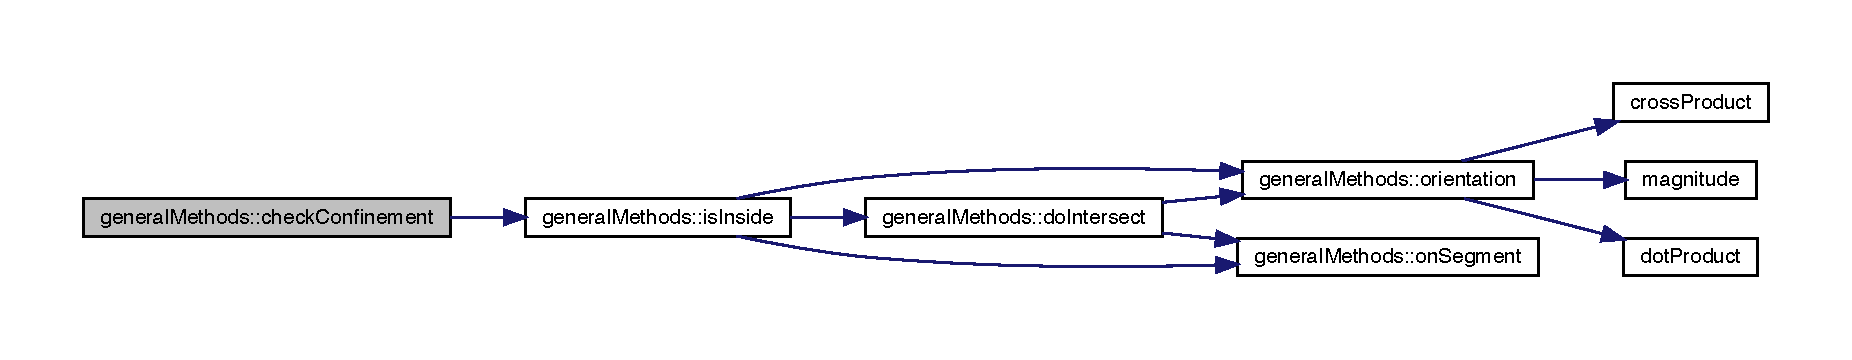
\includegraphics[width=350pt]{namespacegeneral_methods_a2bb810600ec90ec064ea8496ee0ab862_cgraph}
\end{center}
\end{figure}
Here is the caller graph for this function\+:
\nopagebreak
\begin{figure}[H]
\begin{center}
\leavevmode
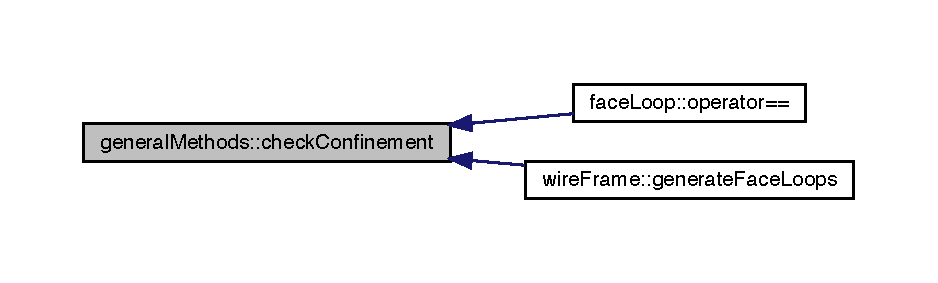
\includegraphics[width=350pt]{namespacegeneral_methods_a2bb810600ec90ec064ea8496ee0ab862_icgraph}
\end{center}
\end{figure}
\mbox{\Hypertarget{namespacegeneral_methods_a508d15a0c76920dc4f98cf8da254f9c4}\label{namespacegeneral_methods_a508d15a0c76920dc4f98cf8da254f9c4}} 
\index{general\+Methods@{general\+Methods}!check\+Coplanar@{check\+Coplanar}}
\index{check\+Coplanar@{check\+Coplanar}!general\+Methods@{general\+Methods}}
\subsubsection{\texorpdfstring{check\+Coplanar()}{checkCoplanar()}}
{\footnotesize\ttfamily bool general\+Methods\+::check\+Coplanar (\begin{DoxyParamCaption}\item[{\mbox{\hyperlink{structedge3_d}{edge3D}}}]{e1,  }\item[{\mbox{\hyperlink{structedge3_d}{edge3D}}}]{e2,  }\item[{\mbox{\hyperlink{structedge3_d}{edge3D}}}]{e3 }\end{DoxyParamCaption})}

check whether two edges coplanar 

Definition at line 163 of file general\+Methods.\+cpp.

Here is the call graph for this function\+:
\nopagebreak
\begin{figure}[H]
\begin{center}
\leavevmode
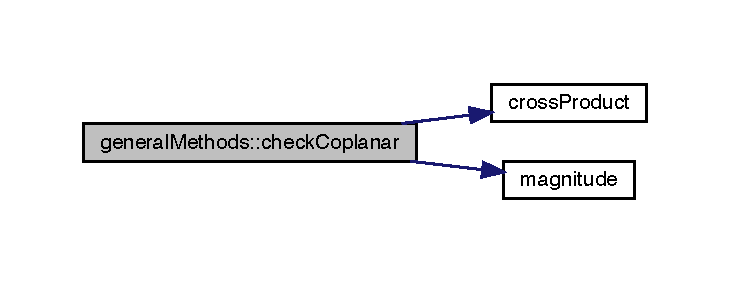
\includegraphics[width=350pt]{namespacegeneral_methods_a508d15a0c76920dc4f98cf8da254f9c4_cgraph}
\end{center}
\end{figure}
Here is the caller graph for this function\+:
\nopagebreak
\begin{figure}[H]
\begin{center}
\leavevmode
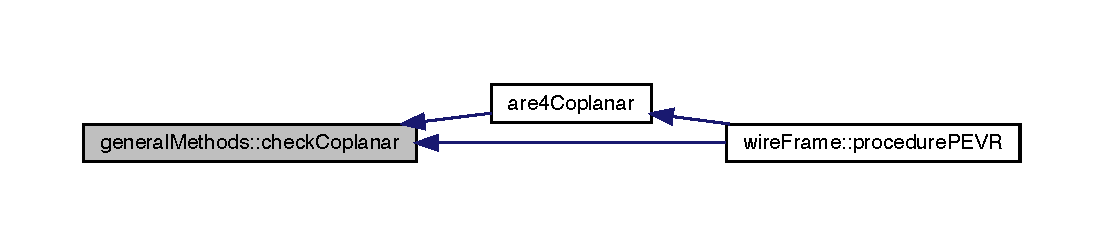
\includegraphics[width=350pt]{namespacegeneral_methods_a508d15a0c76920dc4f98cf8da254f9c4_icgraph}
\end{center}
\end{figure}
\mbox{\Hypertarget{namespacegeneral_methods_a44d97941601f5929b217570ba9027d27}\label{namespacegeneral_methods_a44d97941601f5929b217570ba9027d27}} 
\index{general\+Methods@{general\+Methods}!check\+Hidden@{check\+Hidden}}
\index{check\+Hidden@{check\+Hidden}!general\+Methods@{general\+Methods}}
\subsubsection{\texorpdfstring{check\+Hidden()}{checkHidden()}\hspace{0.1cm}{\footnotesize\ttfamily [1/2]}}
{\footnotesize\ttfamily bool general\+Methods\+::check\+Hidden (\begin{DoxyParamCaption}\item[{\mbox{\hyperlink{structplane}{plane}}}]{p,  }\item[{\mbox{\hyperlink{structedge3_d}{edge3D}}}]{e,  }\item[{float}]{direction }\end{DoxyParamCaption})}

check if plane hides an edge from direction \mbox{\Hypertarget{namespacegeneral_methods_ab4e1b4b0a8b5b7697adddbb27950e639}\label{namespacegeneral_methods_ab4e1b4b0a8b5b7697adddbb27950e639}} 
\index{general\+Methods@{general\+Methods}!check\+Hidden@{check\+Hidden}}
\index{check\+Hidden@{check\+Hidden}!general\+Methods@{general\+Methods}}
\subsubsection{\texorpdfstring{check\+Hidden()}{checkHidden()}\hspace{0.1cm}{\footnotesize\ttfamily [2/2]}}
{\footnotesize\ttfamily bool general\+Methods\+::check\+Hidden (\begin{DoxyParamCaption}\item[{\mbox{\hyperlink{structplane}{plane}}}]{p,  }\item[{\mbox{\hyperlink{structedge3_d}{edge3D}}}]{e,  }\item[{float}]{direction\mbox{[}$\,$\mbox{]} }\end{DoxyParamCaption})}



Definition at line 251 of file general\+Methods.\+cpp.

\mbox{\Hypertarget{namespacegeneral_methods_aa7662b2bcff30f8983da23da5edfc766}\label{namespacegeneral_methods_aa7662b2bcff30f8983da23da5edfc766}} 
\index{general\+Methods@{general\+Methods}!check\+Overlap\+Collinear@{check\+Overlap\+Collinear}}
\index{check\+Overlap\+Collinear@{check\+Overlap\+Collinear}!general\+Methods@{general\+Methods}}
\subsubsection{\texorpdfstring{check\+Overlap\+Collinear()}{checkOverlapCollinear()}}
{\footnotesize\ttfamily bool general\+Methods\+::check\+Overlap\+Collinear (\begin{DoxyParamCaption}\item[{\mbox{\hyperlink{structedge3_d}{edge3D}}}]{e1,  }\item[{\mbox{\hyperlink{structedge3_d}{edge3D}}}]{e2 }\end{DoxyParamCaption})}

-\/-\/-\/-\/-\/-\/-\/-\/-\/-\/-\/------methods of edges-\/-\/-\/-\/-\/-\/-\/-\/-\/-\/-\/-\/-\/-\/-\/-\/-\/-\/-\/-\/-\/-\/-\/------ ~\newline
check if edges overlap and collinear 

Definition at line 126 of file general\+Methods.\+cpp.

Here is the call graph for this function\+:
\nopagebreak
\begin{figure}[H]
\begin{center}
\leavevmode
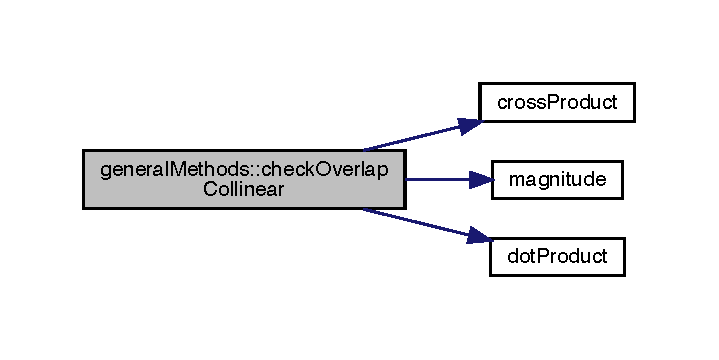
\includegraphics[width=345pt]{namespacegeneral_methods_aa7662b2bcff30f8983da23da5edfc766_cgraph}
\end{center}
\end{figure}
Here is the caller graph for this function\+:
\nopagebreak
\begin{figure}[H]
\begin{center}
\leavevmode
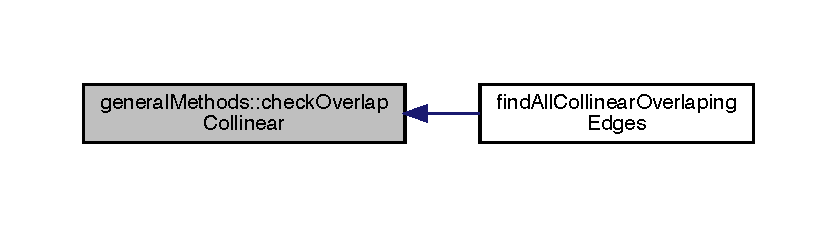
\includegraphics[width=350pt]{namespacegeneral_methods_aa7662b2bcff30f8983da23da5edfc766_icgraph}
\end{center}
\end{figure}
\mbox{\Hypertarget{namespacegeneral_methods_afc8f20af710f8dc24af591015acc1403}\label{namespacegeneral_methods_afc8f20af710f8dc24af591015acc1403}} 
\index{general\+Methods@{general\+Methods}!compare\+Pairs@{compare\+Pairs}}
\index{compare\+Pairs@{compare\+Pairs}!general\+Methods@{general\+Methods}}
\subsubsection{\texorpdfstring{compare\+Pairs()}{comparePairs()}}
{\footnotesize\ttfamily bool general\+Methods\+::compare\+Pairs (\begin{DoxyParamCaption}\item[{\mbox{\hyperlink{structvertex_edge_pair}{vertex\+Edge\+Pair}}}]{pair1,  }\item[{\mbox{\hyperlink{structvertex_edge_pair}{vertex\+Edge\+Pair}}}]{pair2 }\end{DoxyParamCaption})}



Definition at line 95 of file general\+Methods.\+cpp.

Here is the call graph for this function\+:
\nopagebreak
\begin{figure}[H]
\begin{center}
\leavevmode
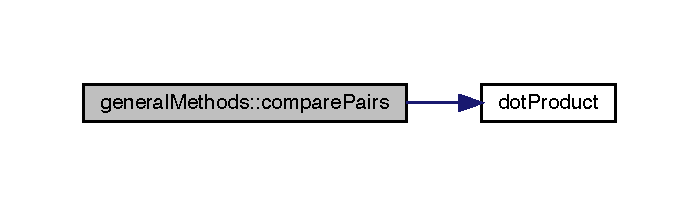
\includegraphics[width=335pt]{namespacegeneral_methods_afc8f20af710f8dc24af591015acc1403_cgraph}
\end{center}
\end{figure}
Here is the caller graph for this function\+:
\nopagebreak
\begin{figure}[H]
\begin{center}
\leavevmode
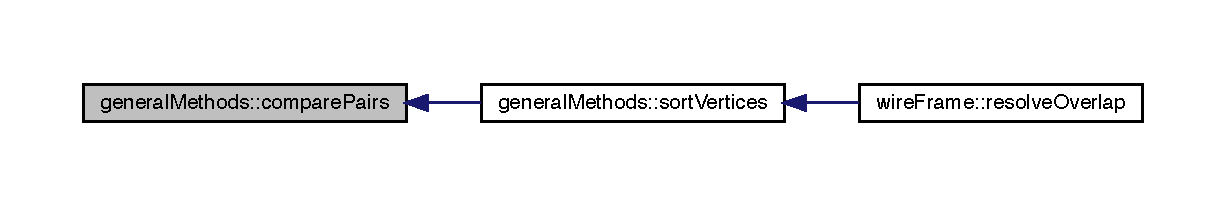
\includegraphics[width=350pt]{namespacegeneral_methods_afc8f20af710f8dc24af591015acc1403_icgraph}
\end{center}
\end{figure}
\mbox{\Hypertarget{namespacegeneral_methods_a56efd049c58aae30a7b0caf39beab615}\label{namespacegeneral_methods_a56efd049c58aae30a7b0caf39beab615}} 
\index{general\+Methods@{general\+Methods}!do\+Intersect@{do\+Intersect}}
\index{do\+Intersect@{do\+Intersect}!general\+Methods@{general\+Methods}}
\subsubsection{\texorpdfstring{do\+Intersect()}{doIntersect()}}
{\footnotesize\ttfamily bool general\+Methods\+::do\+Intersect (\begin{DoxyParamCaption}\item[{\mbox{\hyperlink{structvertex3_d}{vertex3D}}}]{p1,  }\item[{\mbox{\hyperlink{structvertex3_d}{vertex3D}}}]{q1,  }\item[{\mbox{\hyperlink{structvertex3_d}{vertex3D}}}]{p2,  }\item[{\mbox{\hyperlink{structvertex3_d}{vertex3D}}}]{q2,  }\item[{\mbox{\hyperlink{structplane}{plane}}}]{p }\end{DoxyParamCaption})}



Definition at line 295 of file general\+Methods.\+cpp.

Here is the call graph for this function\+:
\nopagebreak
\begin{figure}[H]
\begin{center}
\leavevmode
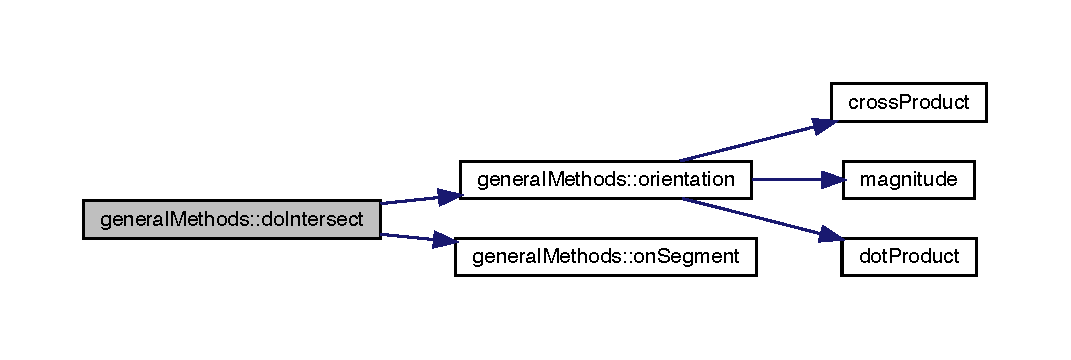
\includegraphics[width=350pt]{namespacegeneral_methods_a56efd049c58aae30a7b0caf39beab615_cgraph}
\end{center}
\end{figure}
Here is the caller graph for this function\+:
\nopagebreak
\begin{figure}[H]
\begin{center}
\leavevmode
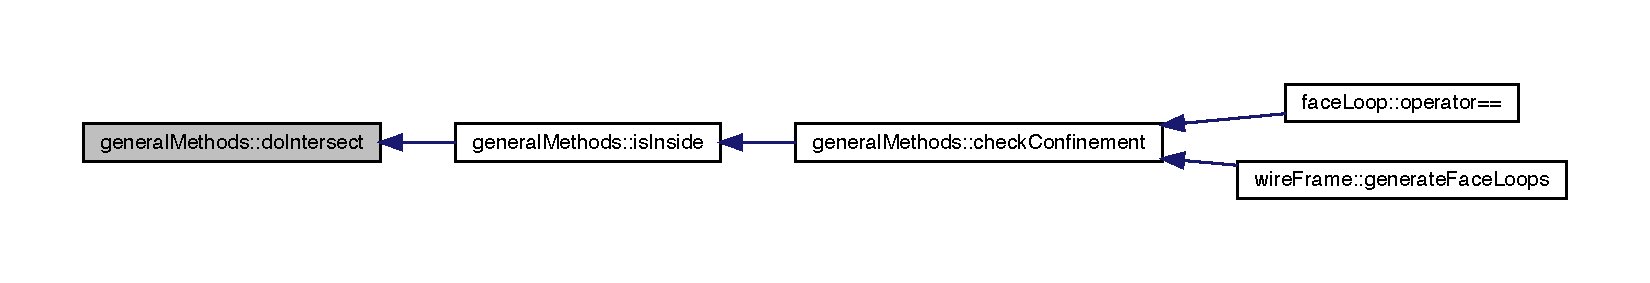
\includegraphics[width=350pt]{namespacegeneral_methods_a56efd049c58aae30a7b0caf39beab615_icgraph}
\end{center}
\end{figure}
\mbox{\Hypertarget{namespacegeneral_methods_a3bc88a001e751ad419e87bf3795ca02b}\label{namespacegeneral_methods_a3bc88a001e751ad419e87bf3795ca02b}} 
\index{general\+Methods@{general\+Methods}!find\+Distance\+Between\+Planes@{find\+Distance\+Between\+Planes}}
\index{find\+Distance\+Between\+Planes@{find\+Distance\+Between\+Planes}!general\+Methods@{general\+Methods}}
\subsubsection{\texorpdfstring{find\+Distance\+Between\+Planes()}{findDistanceBetweenPlanes()}}
{\footnotesize\ttfamily float general\+Methods\+::find\+Distance\+Between\+Planes (\begin{DoxyParamCaption}\item[{\mbox{\hyperlink{structplane}{plane}}}]{p,  }\item[{\mbox{\hyperlink{structplane}{plane}}}]{q }\end{DoxyParamCaption})}

returns distance between two planes 

Definition at line 206 of file general\+Methods.\+cpp.

\mbox{\Hypertarget{namespacegeneral_methods_a9bff72be73e4d6faec798a23b8f28cb9}\label{namespacegeneral_methods_a9bff72be73e4d6faec798a23b8f28cb9}} 
\index{general\+Methods@{general\+Methods}!find\+Edges\+On\+Plane@{find\+Edges\+On\+Plane}}
\index{find\+Edges\+On\+Plane@{find\+Edges\+On\+Plane}!general\+Methods@{general\+Methods}}
\subsubsection{\texorpdfstring{find\+Edges\+On\+Plane()}{findEdgesOnPlane()}}
{\footnotesize\ttfamily std\+::vector$<$ \mbox{\hyperlink{structedge3_d}{edge3D}} $>$ general\+Methods\+::find\+Edges\+On\+Plane (\begin{DoxyParamCaption}\item[{\mbox{\hyperlink{structplane}{plane}}}]{p,  }\item[{std\+::vector$<$ \mbox{\hyperlink{structedge3_d}{edge3D}} $>$}]{e\+List }\end{DoxyParamCaption})}

takes a plane and e\+\_\+list and returns the list of edges on that plane 

Definition at line 227 of file general\+Methods.\+cpp.

Here is the call graph for this function\+:
\nopagebreak
\begin{figure}[H]
\begin{center}
\leavevmode
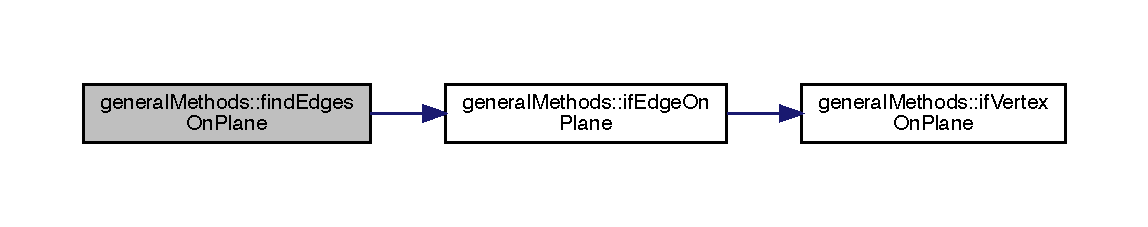
\includegraphics[width=350pt]{namespacegeneral_methods_a9bff72be73e4d6faec798a23b8f28cb9_cgraph}
\end{center}
\end{figure}
Here is the caller graph for this function\+:
\nopagebreak
\begin{figure}[H]
\begin{center}
\leavevmode
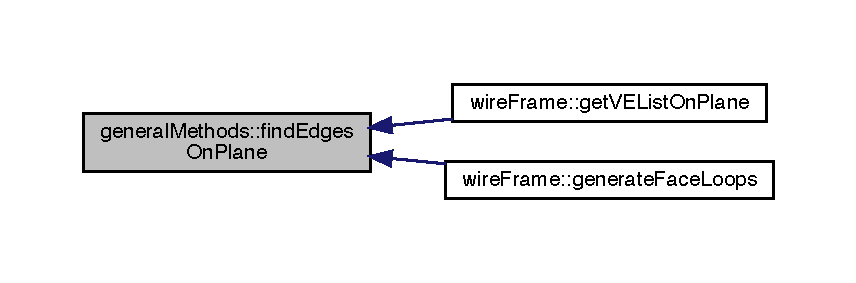
\includegraphics[width=350pt]{namespacegeneral_methods_a9bff72be73e4d6faec798a23b8f28cb9_icgraph}
\end{center}
\end{figure}
\mbox{\Hypertarget{namespacegeneral_methods_aa0669678cf59876e3249ddce7a0d1ce3}\label{namespacegeneral_methods_aa0669678cf59876e3249ddce7a0d1ce3}} 
\index{general\+Methods@{general\+Methods}!find\+Vertices\+On\+Plane@{find\+Vertices\+On\+Plane}}
\index{find\+Vertices\+On\+Plane@{find\+Vertices\+On\+Plane}!general\+Methods@{general\+Methods}}
\subsubsection{\texorpdfstring{find\+Vertices\+On\+Plane()}{findVerticesOnPlane()}}
{\footnotesize\ttfamily std\+::vector$<$ \mbox{\hyperlink{structvertex3_d}{vertex3D}} $>$ general\+Methods\+::find\+Vertices\+On\+Plane (\begin{DoxyParamCaption}\item[{\mbox{\hyperlink{structplane}{plane}}}]{p,  }\item[{std\+::vector$<$ \mbox{\hyperlink{structvertex3_d}{vertex3D}} $>$}]{eop }\end{DoxyParamCaption})}

takes a plane and all vertices and returns all the vertices on that plane 

Definition at line 239 of file general\+Methods.\+cpp.

Here is the call graph for this function\+:
\nopagebreak
\begin{figure}[H]
\begin{center}
\leavevmode
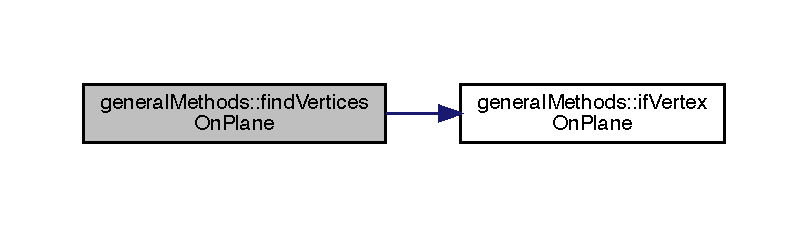
\includegraphics[width=350pt]{namespacegeneral_methods_aa0669678cf59876e3249ddce7a0d1ce3_cgraph}
\end{center}
\end{figure}
Here is the caller graph for this function\+:
\nopagebreak
\begin{figure}[H]
\begin{center}
\leavevmode
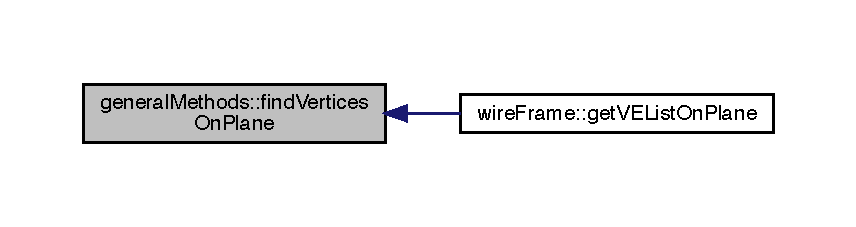
\includegraphics[width=350pt]{namespacegeneral_methods_aa0669678cf59876e3249ddce7a0d1ce3_icgraph}
\end{center}
\end{figure}
\mbox{\Hypertarget{namespacegeneral_methods_a0bd9c59442b6f9c7fd3ae00832ee30df}\label{namespacegeneral_methods_a0bd9c59442b6f9c7fd3ae00832ee30df}} 
\index{general\+Methods@{general\+Methods}!get\+Alpha\+And\+Direction@{get\+Alpha\+And\+Direction}}
\index{get\+Alpha\+And\+Direction@{get\+Alpha\+And\+Direction}!general\+Methods@{general\+Methods}}
\subsubsection{\texorpdfstring{get\+Alpha\+And\+Direction()}{getAlphaAndDirection()}}
{\footnotesize\ttfamily float $\ast$ general\+Methods\+::get\+Alpha\+And\+Direction (\begin{DoxyParamCaption}\item[{\mbox{\hyperlink{classface_loop}{face\+Loop}}}]{flk,  }\item[{\mbox{\hyperlink{classface_loop}{face\+Loop}}}]{fls,  }\item[{\mbox{\hyperlink{structedge3_d}{edge3D}}}]{reference\+Edge }\end{DoxyParamCaption})}

returns alpha as described in paper and whether to select +\+Fs or -\/\+Fs 

Definition at line 417 of file general\+Methods.\+cpp.

Here is the call graph for this function\+:
\nopagebreak
\begin{figure}[H]
\begin{center}
\leavevmode
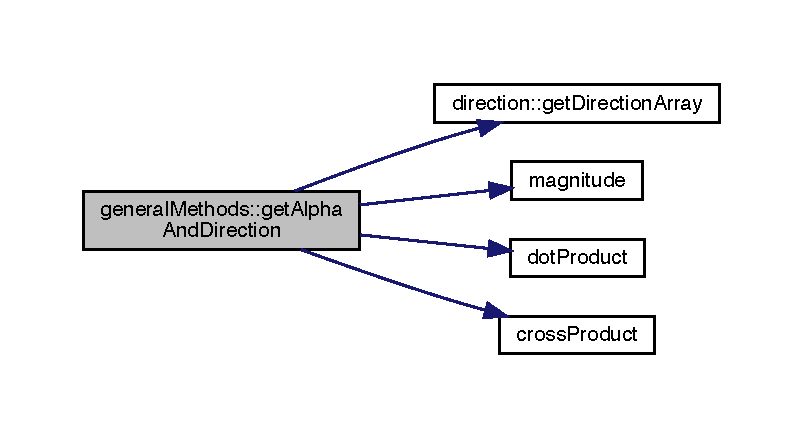
\includegraphics[width=350pt]{namespacegeneral_methods_a0bd9c59442b6f9c7fd3ae00832ee30df_cgraph}
\end{center}
\end{figure}
\mbox{\Hypertarget{namespacegeneral_methods_a4ebb8d563530558e025b62c647045efe}\label{namespacegeneral_methods_a4ebb8d563530558e025b62c647045efe}} 
\index{general\+Methods@{general\+Methods}!get\+If\+Outer@{get\+If\+Outer}}
\index{get\+If\+Outer@{get\+If\+Outer}!general\+Methods@{general\+Methods}}
\subsubsection{\texorpdfstring{get\+If\+Outer()}{getIfOuter()}}
{\footnotesize\ttfamily bool general\+Methods\+::get\+If\+Outer (\begin{DoxyParamCaption}\item[{\mbox{\hyperlink{classbody_loop}{body\+Loop}}}]{b }\end{DoxyParamCaption})}

to determine whether the bodyloop is outer or inner by the method described in paper \mbox{\Hypertarget{namespacegeneral_methods_afe4087e253b318326a0a1578d34b42ca}\label{namespacegeneral_methods_afe4087e253b318326a0a1578d34b42ca}} 
\index{general\+Methods@{general\+Methods}!get\+Reversed\+Face\+Loop@{get\+Reversed\+Face\+Loop}}
\index{get\+Reversed\+Face\+Loop@{get\+Reversed\+Face\+Loop}!general\+Methods@{general\+Methods}}
\subsubsection{\texorpdfstring{get\+Reversed\+Face\+Loop()}{getReversedFaceLoop()}}
{\footnotesize\ttfamily \mbox{\hyperlink{classface_loop}{face\+Loop}} general\+Methods\+::get\+Reversed\+Face\+Loop (\begin{DoxyParamCaption}\item[{\mbox{\hyperlink{classface_loop}{face\+Loop}}}]{faceloop }\end{DoxyParamCaption})}



Definition at line 474 of file general\+Methods.\+cpp.

Here is the call graph for this function\+:
\nopagebreak
\begin{figure}[H]
\begin{center}
\leavevmode
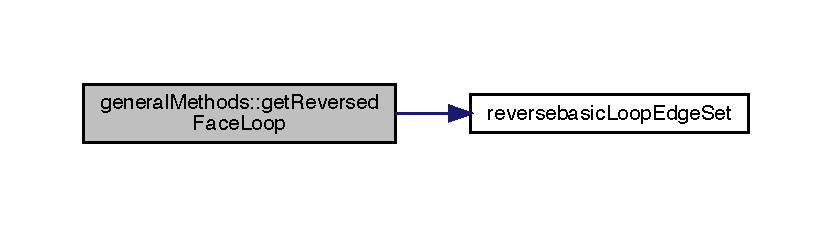
\includegraphics[width=350pt]{namespacegeneral_methods_afe4087e253b318326a0a1578d34b42ca_cgraph}
\end{center}
\end{figure}
Here is the caller graph for this function\+:
\nopagebreak
\begin{figure}[H]
\begin{center}
\leavevmode
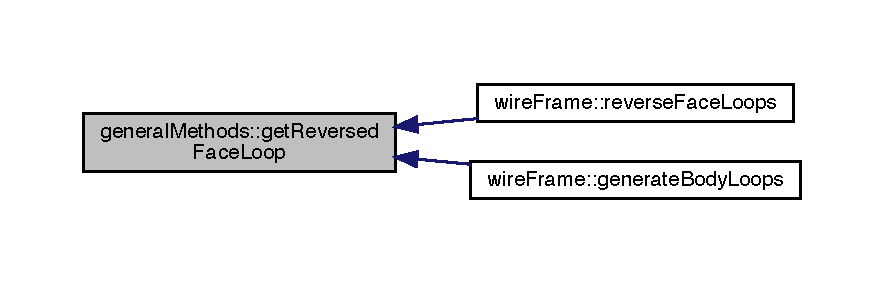
\includegraphics[width=350pt]{namespacegeneral_methods_afe4087e253b318326a0a1578d34b42ca_icgraph}
\end{center}
\end{figure}
\mbox{\Hypertarget{namespacegeneral_methods_a21d2e8c181e8cac3762d9ca1871d2168}\label{namespacegeneral_methods_a21d2e8c181e8cac3762d9ca1871d2168}} 
\index{general\+Methods@{general\+Methods}!if\+Edge\+On\+Plane@{if\+Edge\+On\+Plane}}
\index{if\+Edge\+On\+Plane@{if\+Edge\+On\+Plane}!general\+Methods@{general\+Methods}}
\subsubsection{\texorpdfstring{if\+Edge\+On\+Plane()}{ifEdgeOnPlane()}}
{\footnotesize\ttfamily bool general\+Methods\+::if\+Edge\+On\+Plane (\begin{DoxyParamCaption}\item[{\mbox{\hyperlink{structplane}{plane}}}]{p,  }\item[{\mbox{\hyperlink{structedge3_d}{edge3D}}}]{e }\end{DoxyParamCaption})}

returns distance between a edge and a plane 

Definition at line 221 of file general\+Methods.\+cpp.

Here is the call graph for this function\+:
\nopagebreak
\begin{figure}[H]
\begin{center}
\leavevmode
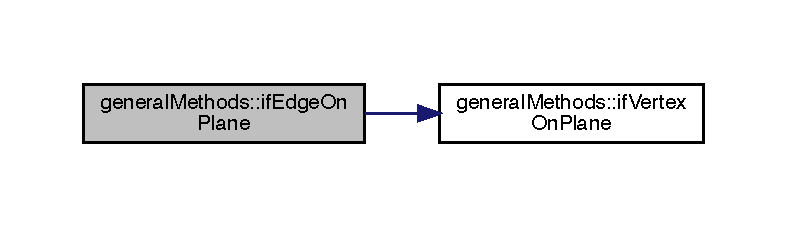
\includegraphics[width=350pt]{namespacegeneral_methods_a21d2e8c181e8cac3762d9ca1871d2168_cgraph}
\end{center}
\end{figure}
Here is the caller graph for this function\+:
\nopagebreak
\begin{figure}[H]
\begin{center}
\leavevmode
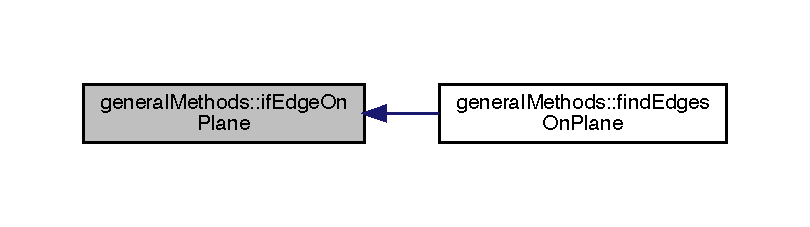
\includegraphics[width=350pt]{namespacegeneral_methods_a21d2e8c181e8cac3762d9ca1871d2168_icgraph}
\end{center}
\end{figure}
\mbox{\Hypertarget{namespacegeneral_methods_a330682bb45234d8de5228a7607d493d2}\label{namespacegeneral_methods_a330682bb45234d8de5228a7607d493d2}} 
\index{general\+Methods@{general\+Methods}!if\+Vertex\+On\+Plane@{if\+Vertex\+On\+Plane}}
\index{if\+Vertex\+On\+Plane@{if\+Vertex\+On\+Plane}!general\+Methods@{general\+Methods}}
\subsubsection{\texorpdfstring{if\+Vertex\+On\+Plane()}{ifVertexOnPlane()}}
{\footnotesize\ttfamily bool general\+Methods\+::if\+Vertex\+On\+Plane (\begin{DoxyParamCaption}\item[{\mbox{\hyperlink{structplane}{plane}}}]{p,  }\item[{\mbox{\hyperlink{structvertex3_d}{vertex3D}}}]{v }\end{DoxyParamCaption})}



Definition at line 215 of file general\+Methods.\+cpp.

Here is the caller graph for this function\+:
\nopagebreak
\begin{figure}[H]
\begin{center}
\leavevmode
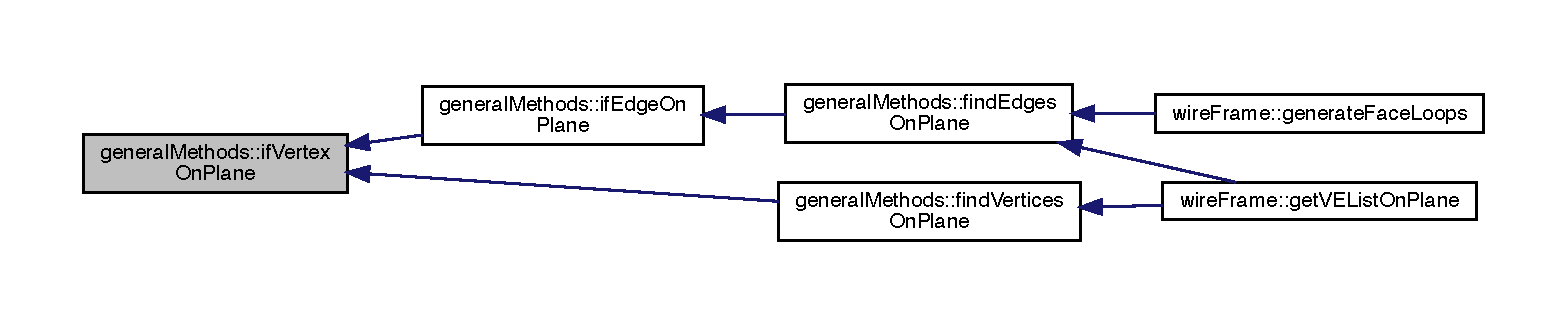
\includegraphics[width=350pt]{namespacegeneral_methods_a330682bb45234d8de5228a7607d493d2_icgraph}
\end{center}
\end{figure}
\mbox{\Hypertarget{namespacegeneral_methods_a27b7ed292415027c495942147e8856b7}\label{namespacegeneral_methods_a27b7ed292415027c495942147e8856b7}} 
\index{general\+Methods@{general\+Methods}!is\+Inside@{is\+Inside}}
\index{is\+Inside@{is\+Inside}!general\+Methods@{general\+Methods}}
\subsubsection{\texorpdfstring{is\+Inside()}{isInside()}}
{\footnotesize\ttfamily bool general\+Methods\+::is\+Inside (\begin{DoxyParamCaption}\item[{std\+::vector$<$ \mbox{\hyperlink{structvertex3_d}{vertex3D}} $>$}]{polygon,  }\item[{int}]{n,  }\item[{\mbox{\hyperlink{structvertex3_d}{vertex3D}}}]{p,  }\item[{\mbox{\hyperlink{structedge3_d}{edge3D}}}]{ref\+Edge,  }\item[{\mbox{\hyperlink{structplane}{plane}}}]{q }\end{DoxyParamCaption})}



Definition at line 323 of file general\+Methods.\+cpp.

Here is the call graph for this function\+:
\nopagebreak
\begin{figure}[H]
\begin{center}
\leavevmode
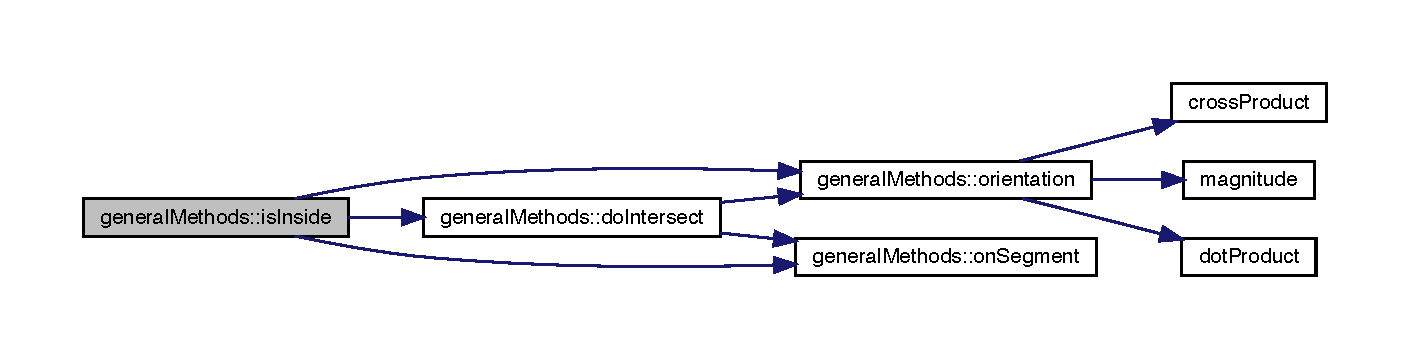
\includegraphics[width=350pt]{namespacegeneral_methods_a27b7ed292415027c495942147e8856b7_cgraph}
\end{center}
\end{figure}
Here is the caller graph for this function\+:
\nopagebreak
\begin{figure}[H]
\begin{center}
\leavevmode
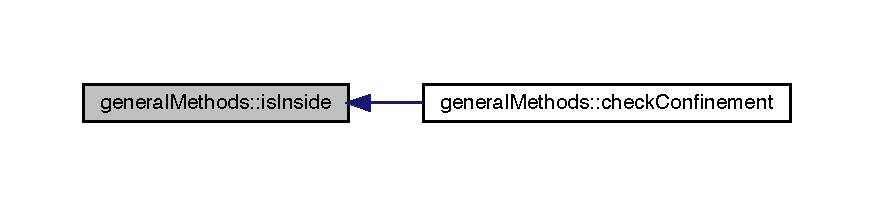
\includegraphics[width=350pt]{namespacegeneral_methods_a27b7ed292415027c495942147e8856b7_icgraph}
\end{center}
\end{figure}
\mbox{\Hypertarget{namespacegeneral_methods_a06d99f1b292d29dbdbe4734847c8d2ee}\label{namespacegeneral_methods_a06d99f1b292d29dbdbe4734847c8d2ee}} 
\index{general\+Methods@{general\+Methods}!make\+Plane@{make\+Plane}}
\index{make\+Plane@{make\+Plane}!general\+Methods@{general\+Methods}}
\subsubsection{\texorpdfstring{make\+Plane()}{makePlane()}}
{\footnotesize\ttfamily \mbox{\hyperlink{structplane}{plane}} general\+Methods\+::make\+Plane (\begin{DoxyParamCaption}\item[{\mbox{\hyperlink{structedge3_d}{edge3D}}}]{e1,  }\item[{\mbox{\hyperlink{structedge3_d}{edge3D}}}]{e2 }\end{DoxyParamCaption})}

take dot procuct ~\newline
~\newline
~\newline
take cross product ~\newline
~\newline
-\/-\/-\/-\/-\/-\/-\/-\/-\/-\/-\/------methods of planes-\/-\/-\/-\/-\/-\/-\/-\/-\/-\/-\/-\/-\/-\/-\/-\/-\/-\/-\/-\/-\/-\/------ ~\newline
make a plane using two adjacent edges 

Definition at line 175 of file general\+Methods.\+cpp.

Here is the call graph for this function\+:
\nopagebreak
\begin{figure}[H]
\begin{center}
\leavevmode
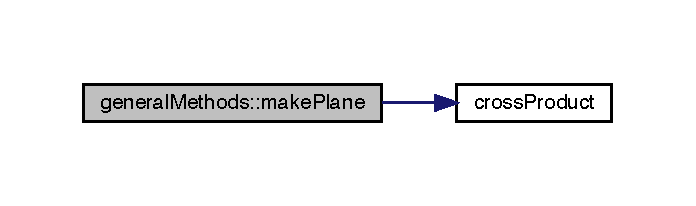
\includegraphics[width=334pt]{namespacegeneral_methods_a06d99f1b292d29dbdbe4734847c8d2ee_cgraph}
\end{center}
\end{figure}
\mbox{\Hypertarget{namespacegeneral_methods_a557bf2257d6658862b42124035aa9588}\label{namespacegeneral_methods_a557bf2257d6658862b42124035aa9588}} 
\index{general\+Methods@{general\+Methods}!on\+Segment@{on\+Segment}}
\index{on\+Segment@{on\+Segment}!general\+Methods@{general\+Methods}}
\subsubsection{\texorpdfstring{on\+Segment()}{onSegment()}}
{\footnotesize\ttfamily bool general\+Methods\+::on\+Segment (\begin{DoxyParamCaption}\item[{\mbox{\hyperlink{structvertex3_d}{vertex3D}}}]{v,  }\item[{\mbox{\hyperlink{structedge3_d}{edge3D}}}]{edge }\end{DoxyParamCaption})}



Definition at line 268 of file general\+Methods.\+cpp.

Here is the caller graph for this function\+:
\nopagebreak
\begin{figure}[H]
\begin{center}
\leavevmode
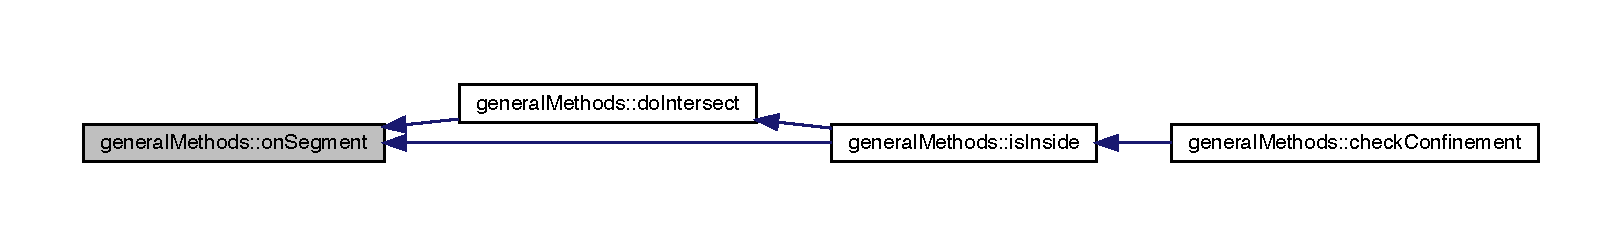
\includegraphics[width=350pt]{namespacegeneral_methods_a557bf2257d6658862b42124035aa9588_icgraph}
\end{center}
\end{figure}
\mbox{\Hypertarget{namespacegeneral_methods_a7bfbfb2a02328d76e70f66fedd57c4ef}\label{namespacegeneral_methods_a7bfbfb2a02328d76e70f66fedd57c4ef}} 
\index{general\+Methods@{general\+Methods}!orientation@{orientation}}
\index{orientation@{orientation}!general\+Methods@{general\+Methods}}
\subsubsection{\texorpdfstring{orientation()}{orientation()}}
{\footnotesize\ttfamily int general\+Methods\+::orientation (\begin{DoxyParamCaption}\item[{\mbox{\hyperlink{structvertex3_d}{vertex3D}}}]{p,  }\item[{\mbox{\hyperlink{structvertex3_d}{vertex3D}}}]{q,  }\item[{\mbox{\hyperlink{structvertex3_d}{vertex3D}}}]{r,  }\item[{\mbox{\hyperlink{structplane}{plane}}}]{s }\end{DoxyParamCaption})}



Definition at line 277 of file general\+Methods.\+cpp.

Here is the call graph for this function\+:
\nopagebreak
\begin{figure}[H]
\begin{center}
\leavevmode
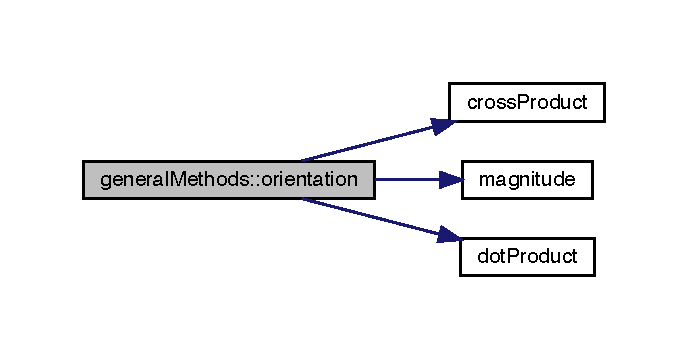
\includegraphics[width=330pt]{namespacegeneral_methods_a7bfbfb2a02328d76e70f66fedd57c4ef_cgraph}
\end{center}
\end{figure}
Here is the caller graph for this function\+:
\nopagebreak
\begin{figure}[H]
\begin{center}
\leavevmode
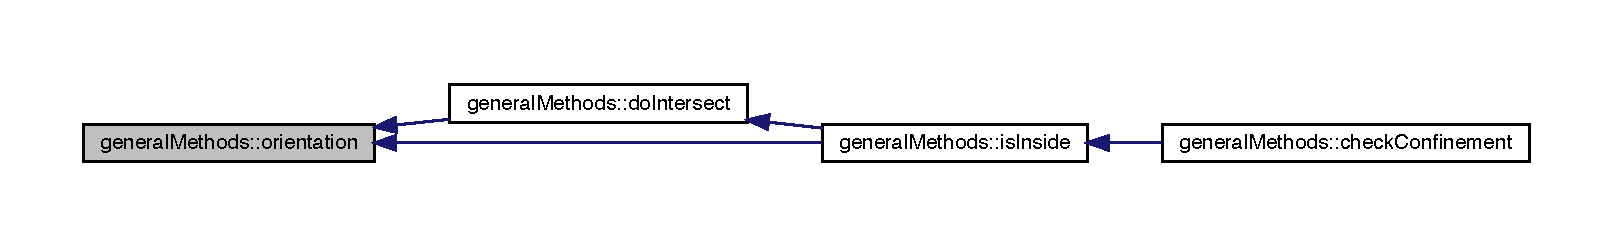
\includegraphics[width=350pt]{namespacegeneral_methods_a7bfbfb2a02328d76e70f66fedd57c4ef_icgraph}
\end{center}
\end{figure}
\mbox{\Hypertarget{namespacegeneral_methods_a3c49599a5ba8f2c41f2ef542bde19765}\label{namespacegeneral_methods_a3c49599a5ba8f2c41f2ef542bde19765}} 
\index{general\+Methods@{general\+Methods}!plane\+Equal@{plane\+Equal}}
\index{plane\+Equal@{plane\+Equal}!general\+Methods@{general\+Methods}}
\subsubsection{\texorpdfstring{plane\+Equal()}{planeEqual()}}
{\footnotesize\ttfamily bool general\+Methods\+::plane\+Equal (\begin{DoxyParamCaption}\item[{\mbox{\hyperlink{structplane}{plane}}}]{p1,  }\item[{\mbox{\hyperlink{structplane}{plane}}}]{p2 }\end{DoxyParamCaption})}



Definition at line 188 of file general\+Methods.\+cpp.

\mbox{\Hypertarget{namespacegeneral_methods_af9a1c28dacf89e746b51916fe178ce1a}\label{namespacegeneral_methods_af9a1c28dacf89e746b51916fe178ce1a}} 
\index{general\+Methods@{general\+Methods}!print\+Edge@{print\+Edge}}
\index{print\+Edge@{print\+Edge}!general\+Methods@{general\+Methods}}
\subsubsection{\texorpdfstring{print\+Edge()}{printEdge()}}
{\footnotesize\ttfamily void general\+Methods\+::print\+Edge (\begin{DoxyParamCaption}\item[{\mbox{\hyperlink{structedge3_d}{edge3D}}}]{i }\end{DoxyParamCaption})}

~\newline
print the edge\+List

~\newline
print the edge\+List

Definition at line 36 of file general\+Methods.\+cpp.

Here is the call graph for this function\+:
\nopagebreak
\begin{figure}[H]
\begin{center}
\leavevmode
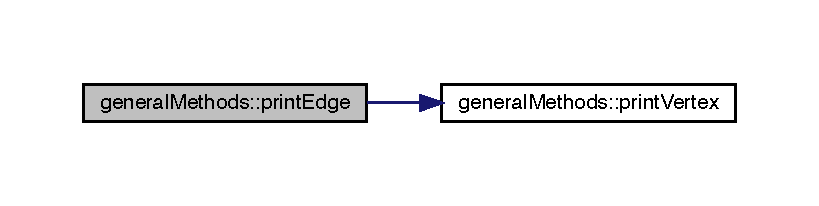
\includegraphics[width=350pt]{namespacegeneral_methods_af9a1c28dacf89e746b51916fe178ce1a_cgraph}
\end{center}
\end{figure}
\mbox{\Hypertarget{namespacegeneral_methods_ab6b6f8a5d92b39ead6c97ec0917b75a4}\label{namespacegeneral_methods_ab6b6f8a5d92b39ead6c97ec0917b75a4}} 
\index{general\+Methods@{general\+Methods}!print\+Edge\+List@{print\+Edge\+List}}
\index{print\+Edge\+List@{print\+Edge\+List}!general\+Methods@{general\+Methods}}
\subsubsection{\texorpdfstring{print\+Edge\+List()}{printEdgeList()}}
{\footnotesize\ttfamily void general\+Methods\+::print\+Edge\+List (\begin{DoxyParamCaption}\item[{vector$<$ \mbox{\hyperlink{structedge3_d}{edge3D}} $>$}]{e }\end{DoxyParamCaption})}

~\newline
print the edge\+List

~\newline
print the edge\+List

Definition at line 43 of file general\+Methods.\+cpp.

Here is the call graph for this function\+:
\nopagebreak
\begin{figure}[H]
\begin{center}
\leavevmode
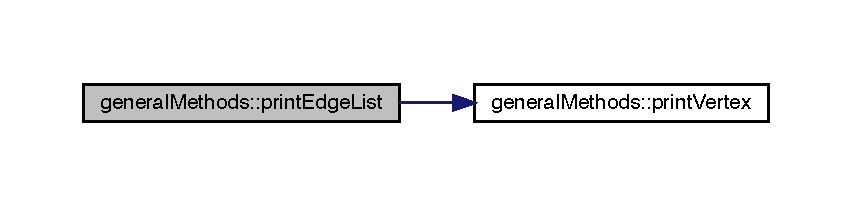
\includegraphics[width=350pt]{namespacegeneral_methods_ab6b6f8a5d92b39ead6c97ec0917b75a4_cgraph}
\end{center}
\end{figure}
Here is the caller graph for this function\+:
\nopagebreak
\begin{figure}[H]
\begin{center}
\leavevmode
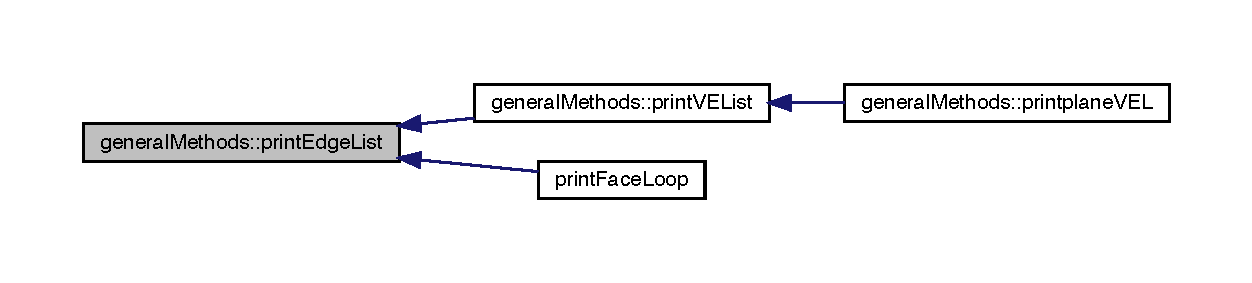
\includegraphics[width=350pt]{namespacegeneral_methods_ab6b6f8a5d92b39ead6c97ec0917b75a4_icgraph}
\end{center}
\end{figure}
\mbox{\Hypertarget{namespacegeneral_methods_a3474d24f9f545407bb5f73250a5e19d7}\label{namespacegeneral_methods_a3474d24f9f545407bb5f73250a5e19d7}} 
\index{general\+Methods@{general\+Methods}!print\+Plane@{print\+Plane}}
\index{print\+Plane@{print\+Plane}!general\+Methods@{general\+Methods}}
\subsubsection{\texorpdfstring{print\+Plane()}{printPlane()}}
{\footnotesize\ttfamily void general\+Methods\+::print\+Plane (\begin{DoxyParamCaption}\item[{\mbox{\hyperlink{structplane}{plane}}}]{p }\end{DoxyParamCaption})}



Definition at line 53 of file general\+Methods.\+cpp.

Here is the caller graph for this function\+:
\nopagebreak
\begin{figure}[H]
\begin{center}
\leavevmode
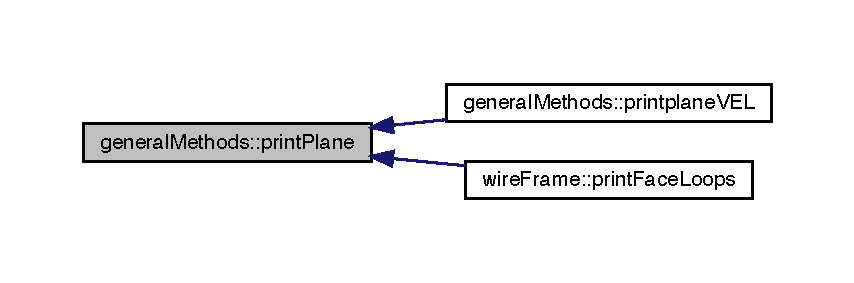
\includegraphics[width=350pt]{namespacegeneral_methods_a3474d24f9f545407bb5f73250a5e19d7_icgraph}
\end{center}
\end{figure}
\mbox{\Hypertarget{namespacegeneral_methods_aa7c9b8abc94ae6b08d2cf083a08eaf21}\label{namespacegeneral_methods_aa7c9b8abc94ae6b08d2cf083a08eaf21}} 
\index{general\+Methods@{general\+Methods}!print\+Planes@{print\+Planes}}
\index{print\+Planes@{print\+Planes}!general\+Methods@{general\+Methods}}
\subsubsection{\texorpdfstring{print\+Planes()}{printPlanes()}}
{\footnotesize\ttfamily void general\+Methods\+::print\+Planes (\begin{DoxyParamCaption}\item[{vector$<$ \mbox{\hyperlink{structplane}{plane}} $>$}]{p }\end{DoxyParamCaption})}



Definition at line 57 of file general\+Methods.\+cpp.

\mbox{\Hypertarget{namespacegeneral_methods_adc8e104a2f2ed35a22be9a68051ec38d}\label{namespacegeneral_methods_adc8e104a2f2ed35a22be9a68051ec38d}} 
\index{general\+Methods@{general\+Methods}!printplane\+V\+EL@{printplane\+V\+EL}}
\index{printplane\+V\+EL@{printplane\+V\+EL}!general\+Methods@{general\+Methods}}
\subsubsection{\texorpdfstring{printplane\+V\+E\+L()}{printplaneVEL()}}
{\footnotesize\ttfamily void general\+Methods\+::printplane\+V\+EL (\begin{DoxyParamCaption}\item[{\mbox{\hyperlink{structplane_v_e_l}{plane\+V\+EL}}}]{p }\end{DoxyParamCaption})}



Definition at line 71 of file general\+Methods.\+cpp.

Here is the call graph for this function\+:
\nopagebreak
\begin{figure}[H]
\begin{center}
\leavevmode
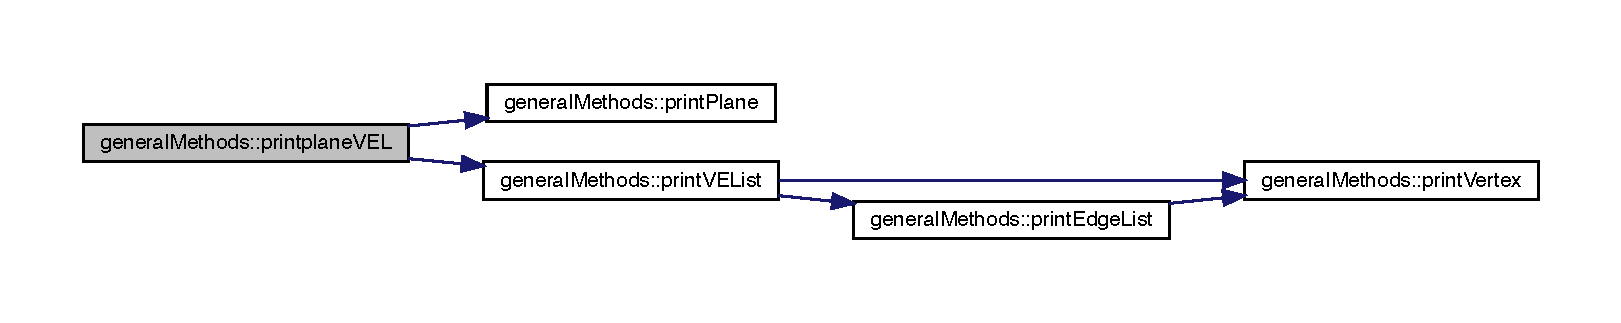
\includegraphics[width=350pt]{namespacegeneral_methods_adc8e104a2f2ed35a22be9a68051ec38d_cgraph}
\end{center}
\end{figure}
\mbox{\Hypertarget{namespacegeneral_methods_a60a9e0ba058824389fc703dc2dbbb7e3}\label{namespacegeneral_methods_a60a9e0ba058824389fc703dc2dbbb7e3}} 
\index{general\+Methods@{general\+Methods}!print\+V\+E\+List@{print\+V\+E\+List}}
\index{print\+V\+E\+List@{print\+V\+E\+List}!general\+Methods@{general\+Methods}}
\subsubsection{\texorpdfstring{print\+V\+E\+List()}{printVEList()}}
{\footnotesize\ttfamily void general\+Methods\+::print\+V\+E\+List (\begin{DoxyParamCaption}\item[{\mbox{\hyperlink{structvertex_edge_list}{vertex\+Edge\+List}}}]{ve\+List }\end{DoxyParamCaption})}



Definition at line 63 of file general\+Methods.\+cpp.

Here is the call graph for this function\+:
\nopagebreak
\begin{figure}[H]
\begin{center}
\leavevmode
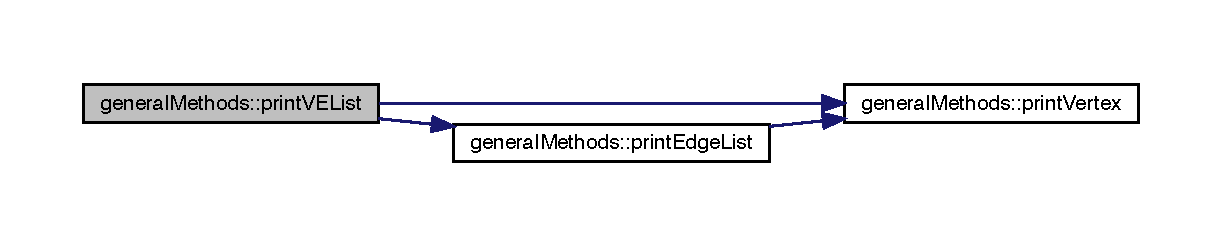
\includegraphics[width=350pt]{namespacegeneral_methods_a60a9e0ba058824389fc703dc2dbbb7e3_cgraph}
\end{center}
\end{figure}
Here is the caller graph for this function\+:
\nopagebreak
\begin{figure}[H]
\begin{center}
\leavevmode
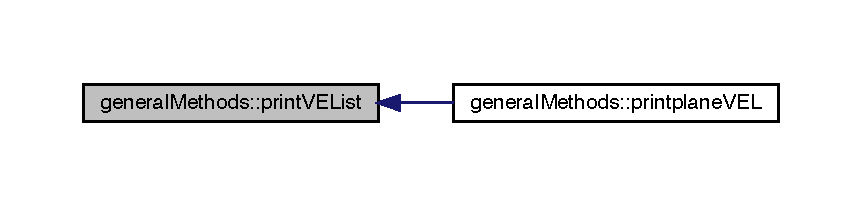
\includegraphics[width=350pt]{namespacegeneral_methods_a60a9e0ba058824389fc703dc2dbbb7e3_icgraph}
\end{center}
\end{figure}
\mbox{\Hypertarget{namespacegeneral_methods_a694306c7472ee1bbfb3c90c0f3d5453a}\label{namespacegeneral_methods_a694306c7472ee1bbfb3c90c0f3d5453a}} 
\index{general\+Methods@{general\+Methods}!print\+Vertex@{print\+Vertex}}
\index{print\+Vertex@{print\+Vertex}!general\+Methods@{general\+Methods}}
\subsubsection{\texorpdfstring{print\+Vertex()}{printVertex()}}
{\footnotesize\ttfamily void general\+Methods\+::print\+Vertex (\begin{DoxyParamCaption}\item[{\mbox{\hyperlink{structvertex3_d}{vertex3D}}}]{i }\end{DoxyParamCaption})}



print methods 

print methods 

Definition at line 20 of file general\+Methods.\+cpp.

Here is the caller graph for this function\+:
\nopagebreak
\begin{figure}[H]
\begin{center}
\leavevmode
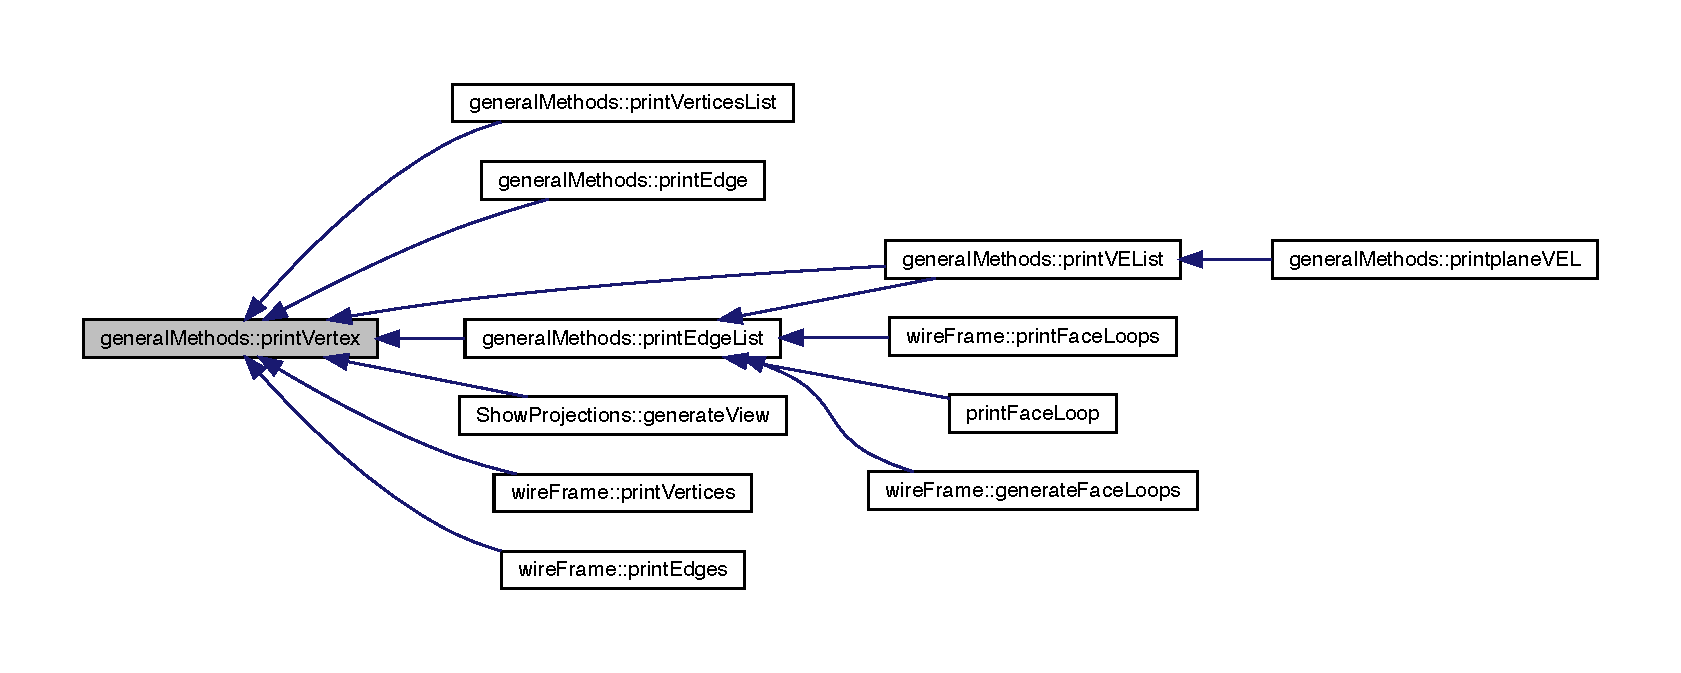
\includegraphics[width=350pt]{namespacegeneral_methods_a694306c7472ee1bbfb3c90c0f3d5453a_icgraph}
\end{center}
\end{figure}
\mbox{\Hypertarget{namespacegeneral_methods_a9cbf7d7c2019f0e2b6f9773b687b50cd}\label{namespacegeneral_methods_a9cbf7d7c2019f0e2b6f9773b687b50cd}} 
\index{general\+Methods@{general\+Methods}!print\+Vertices\+List@{print\+Vertices\+List}}
\index{print\+Vertices\+List@{print\+Vertices\+List}!general\+Methods@{general\+Methods}}
\subsubsection{\texorpdfstring{print\+Vertices\+List()}{printVerticesList()}}
{\footnotesize\ttfamily void general\+Methods\+::print\+Vertices\+List (\begin{DoxyParamCaption}\item[{vector$<$ \mbox{\hyperlink{structvertex3_d}{vertex3D}} $>$}]{v }\end{DoxyParamCaption})}

print the vertex\+List

print the vertex\+List

Definition at line 24 of file general\+Methods.\+cpp.

Here is the call graph for this function\+:
\nopagebreak
\begin{figure}[H]
\begin{center}
\leavevmode
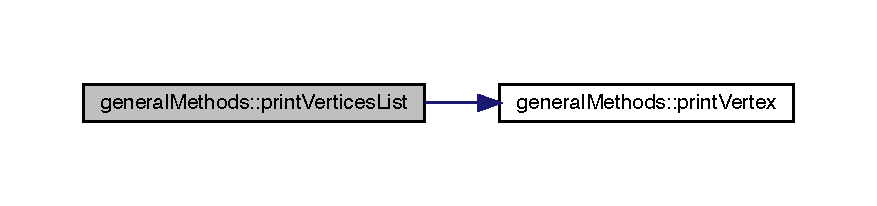
\includegraphics[width=350pt]{namespacegeneral_methods_a9cbf7d7c2019f0e2b6f9773b687b50cd_cgraph}
\end{center}
\end{figure}
\mbox{\Hypertarget{namespacegeneral_methods_a13072e8b14fcea9ae253085569062158}\label{namespacegeneral_methods_a13072e8b14fcea9ae253085569062158}} 
\index{general\+Methods@{general\+Methods}!remove\+Duplicate@{remove\+Duplicate}}
\index{remove\+Duplicate@{remove\+Duplicate}!general\+Methods@{general\+Methods}}
\subsubsection{\texorpdfstring{remove\+Duplicate()}{removeDuplicate()}}
{\footnotesize\ttfamily std\+::vector$<$ \mbox{\hyperlink{structplane}{plane}} $>$ general\+Methods\+::remove\+Duplicate (\begin{DoxyParamCaption}\item[{std\+::vector$<$ \mbox{\hyperlink{structplane}{plane}} $>$}]{v }\end{DoxyParamCaption})}

use this to make all possible planes and then remove the duplicate ones 

Definition at line 195 of file general\+Methods.\+cpp.

\mbox{\Hypertarget{namespacegeneral_methods_ace3487740f3b46dce9e0357366abf9ed}\label{namespacegeneral_methods_ace3487740f3b46dce9e0357366abf9ed}} 
\index{general\+Methods@{general\+Methods}!sort\+Vertices@{sort\+Vertices}}
\index{sort\+Vertices@{sort\+Vertices}!general\+Methods@{general\+Methods}}
\subsubsection{\texorpdfstring{sort\+Vertices()}{sortVertices()}}
{\footnotesize\ttfamily std\+::vector$<$ \mbox{\hyperlink{structvertex3_d}{vertex3D}} $>$ general\+Methods\+::sort\+Vertices (\begin{DoxyParamCaption}\item[{std\+::vector$<$ \mbox{\hyperlink{structvertex3_d}{vertex3D}} $>$}]{V,  }\item[{\mbox{\hyperlink{structedge3_d}{edge3D}}}]{e }\end{DoxyParamCaption})}

-\/-\/-\/-\/-\/-\/-\/-\/-\/-\/-\/------methods of vertices-\/-\/-\/-\/-\/-\/-\/-\/-\/-\/-\/-\/-\/-\/-\/-\/-\/-\/-\/-\/------ ~\newline
sort the vertices along a given edge 

Definition at line 105 of file general\+Methods.\+cpp.

Here is the call graph for this function\+:
\nopagebreak
\begin{figure}[H]
\begin{center}
\leavevmode
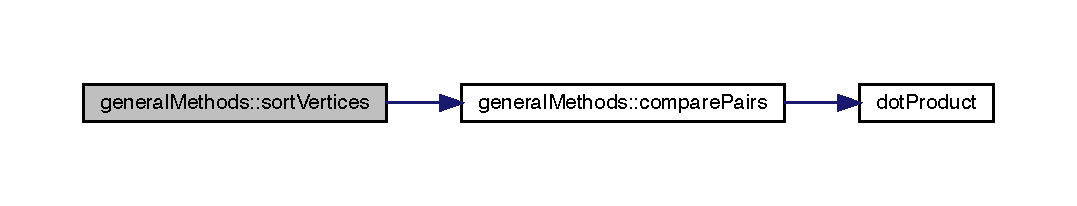
\includegraphics[width=350pt]{namespacegeneral_methods_ace3487740f3b46dce9e0357366abf9ed_cgraph}
\end{center}
\end{figure}
Here is the caller graph for this function\+:
\nopagebreak
\begin{figure}[H]
\begin{center}
\leavevmode
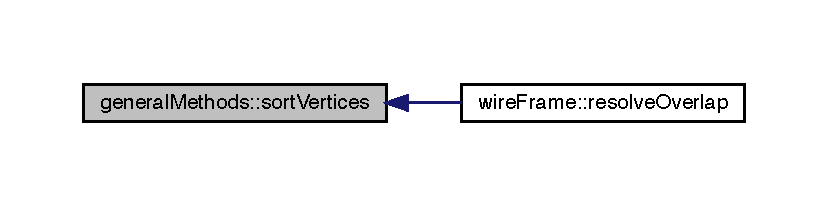
\includegraphics[width=350pt]{namespacegeneral_methods_ace3487740f3b46dce9e0357366abf9ed_icgraph}
\end{center}
\end{figure}

\chapter{Class Documentation}
\hypertarget{structqt__meta__stringdata___main_window__t}{}\section{qt\+\_\+meta\+\_\+stringdata\+\_\+\+Main\+Window\+\_\+t Struct Reference}
\label{structqt__meta__stringdata___main_window__t}\index{qt\+\_\+meta\+\_\+stringdata\+\_\+\+Main\+Window\+\_\+t@{qt\+\_\+meta\+\_\+stringdata\+\_\+\+Main\+Window\+\_\+t}}
\subsection*{Public Attributes}
\begin{DoxyCompactItemize}
\item 
Q\+Byte\+Array\+Data \mbox{\hyperlink{structqt__meta__stringdata___main_window__t_a092956d0ba2e51cd73092e8a5ebb6ce6}{data}} \mbox{[}8\mbox{]}
\item 
char \mbox{\hyperlink{structqt__meta__stringdata___main_window__t_a17b51b6af12b7f5ebb4f7b55545039db}{stringdata0}} \mbox{[}145\mbox{]}
\end{DoxyCompactItemize}


\subsection{Detailed Description}


Definition at line 21 of file moc\+\_\+mainwindow.\+cpp.



\subsection{Member Data Documentation}
\mbox{\Hypertarget{structqt__meta__stringdata___main_window__t_a092956d0ba2e51cd73092e8a5ebb6ce6}\label{structqt__meta__stringdata___main_window__t_a092956d0ba2e51cd73092e8a5ebb6ce6}} 
\index{qt\+\_\+meta\+\_\+stringdata\+\_\+\+Main\+Window\+\_\+t@{qt\+\_\+meta\+\_\+stringdata\+\_\+\+Main\+Window\+\_\+t}!data@{data}}
\index{data@{data}!qt\+\_\+meta\+\_\+stringdata\+\_\+\+Main\+Window\+\_\+t@{qt\+\_\+meta\+\_\+stringdata\+\_\+\+Main\+Window\+\_\+t}}
\subsubsection{\texorpdfstring{data}{data}}
{\footnotesize\ttfamily Q\+Byte\+Array\+Data qt\+\_\+meta\+\_\+stringdata\+\_\+\+Main\+Window\+\_\+t\+::data}



Definition at line 22 of file moc\+\_\+mainwindow.\+cpp.

\mbox{\Hypertarget{structqt__meta__stringdata___main_window__t_a17b51b6af12b7f5ebb4f7b55545039db}\label{structqt__meta__stringdata___main_window__t_a17b51b6af12b7f5ebb4f7b55545039db}} 
\index{qt\+\_\+meta\+\_\+stringdata\+\_\+\+Main\+Window\+\_\+t@{qt\+\_\+meta\+\_\+stringdata\+\_\+\+Main\+Window\+\_\+t}!stringdata0@{stringdata0}}
\index{stringdata0@{stringdata0}!qt\+\_\+meta\+\_\+stringdata\+\_\+\+Main\+Window\+\_\+t@{qt\+\_\+meta\+\_\+stringdata\+\_\+\+Main\+Window\+\_\+t}}
\subsubsection{\texorpdfstring{stringdata0}{stringdata0}}
{\footnotesize\ttfamily char qt\+\_\+meta\+\_\+stringdata\+\_\+\+Main\+Window\+\_\+t\+::stringdata0}



Definition at line 23 of file moc\+\_\+mainwindow.\+cpp.



The documentation for this struct was generated from the following file\+:\begin{DoxyCompactItemize}
\item 
build/\mbox{\hyperlink{build_2moc__mainwindow_8cpp}{moc\+\_\+mainwindow.\+cpp}}\end{DoxyCompactItemize}

\hypertarget{structqt__meta__stringdata___options__t}{}\section{qt\+\_\+meta\+\_\+stringdata\+\_\+\+Options\+\_\+t Struct Reference}
\label{structqt__meta__stringdata___options__t}\index{qt\+\_\+meta\+\_\+stringdata\+\_\+\+Options\+\_\+t@{qt\+\_\+meta\+\_\+stringdata\+\_\+\+Options\+\_\+t}}
\subsection*{Public Attributes}
\begin{DoxyCompactItemize}
\item 
Q\+Byte\+Array\+Data \mbox{\hyperlink{structqt__meta__stringdata___options__t_ad630fb0469c0871580fa3053b9b09bb8}{data}} \mbox{[}1\mbox{]}
\item 
char \mbox{\hyperlink{structqt__meta__stringdata___options__t_a1c10b521fc0bfc89e2ad3c4ae2bc0b34}{stringdata0}} \mbox{[}8\mbox{]}
\end{DoxyCompactItemize}


\subsection{Detailed Description}


Definition at line 21 of file moc\+\_\+options.\+cpp.



\subsection{Member Data Documentation}
\mbox{\Hypertarget{structqt__meta__stringdata___options__t_ad630fb0469c0871580fa3053b9b09bb8}\label{structqt__meta__stringdata___options__t_ad630fb0469c0871580fa3053b9b09bb8}} 
\index{qt\+\_\+meta\+\_\+stringdata\+\_\+\+Options\+\_\+t@{qt\+\_\+meta\+\_\+stringdata\+\_\+\+Options\+\_\+t}!data@{data}}
\index{data@{data}!qt\+\_\+meta\+\_\+stringdata\+\_\+\+Options\+\_\+t@{qt\+\_\+meta\+\_\+stringdata\+\_\+\+Options\+\_\+t}}
\subsubsection{\texorpdfstring{data}{data}}
{\footnotesize\ttfamily Q\+Byte\+Array\+Data qt\+\_\+meta\+\_\+stringdata\+\_\+\+Options\+\_\+t\+::data}



Definition at line 22 of file moc\+\_\+options.\+cpp.

\mbox{\Hypertarget{structqt__meta__stringdata___options__t_a1c10b521fc0bfc89e2ad3c4ae2bc0b34}\label{structqt__meta__stringdata___options__t_a1c10b521fc0bfc89e2ad3c4ae2bc0b34}} 
\index{qt\+\_\+meta\+\_\+stringdata\+\_\+\+Options\+\_\+t@{qt\+\_\+meta\+\_\+stringdata\+\_\+\+Options\+\_\+t}!stringdata0@{stringdata0}}
\index{stringdata0@{stringdata0}!qt\+\_\+meta\+\_\+stringdata\+\_\+\+Options\+\_\+t@{qt\+\_\+meta\+\_\+stringdata\+\_\+\+Options\+\_\+t}}
\subsubsection{\texorpdfstring{stringdata0}{stringdata0}}
{\footnotesize\ttfamily char qt\+\_\+meta\+\_\+stringdata\+\_\+\+Options\+\_\+t\+::stringdata0}



Definition at line 23 of file moc\+\_\+options.\+cpp.



The documentation for this struct was generated from the following file\+:\begin{DoxyCompactItemize}
\item 
build/\mbox{\hyperlink{build_2moc__options_8cpp}{moc\+\_\+options.\+cpp}}\end{DoxyCompactItemize}

\hypertarget{structqt__meta__stringdata___selection__t}{}\section{qt\+\_\+meta\+\_\+stringdata\+\_\+\+Selection\+\_\+t Struct Reference}
\label{structqt__meta__stringdata___selection__t}\index{qt\+\_\+meta\+\_\+stringdata\+\_\+\+Selection\+\_\+t@{qt\+\_\+meta\+\_\+stringdata\+\_\+\+Selection\+\_\+t}}
\subsection*{Public Attributes}
\begin{DoxyCompactItemize}
\item 
Q\+Byte\+Array\+Data \mbox{\hyperlink{structqt__meta__stringdata___selection__t_ac153f153e95caf143389140d4e56cd5b}{data}} \mbox{[}4\mbox{]}
\item 
char \mbox{\hyperlink{structqt__meta__stringdata___selection__t_aebaf48c958bfda11e969b41fc7e0a2eb}{stringdata0}} \mbox{[}52\mbox{]}
\end{DoxyCompactItemize}


\subsection{Detailed Description}


Definition at line 21 of file moc\+\_\+selection.\+cpp.



\subsection{Member Data Documentation}
\mbox{\Hypertarget{structqt__meta__stringdata___selection__t_ac153f153e95caf143389140d4e56cd5b}\label{structqt__meta__stringdata___selection__t_ac153f153e95caf143389140d4e56cd5b}} 
\index{qt\+\_\+meta\+\_\+stringdata\+\_\+\+Selection\+\_\+t@{qt\+\_\+meta\+\_\+stringdata\+\_\+\+Selection\+\_\+t}!data@{data}}
\index{data@{data}!qt\+\_\+meta\+\_\+stringdata\+\_\+\+Selection\+\_\+t@{qt\+\_\+meta\+\_\+stringdata\+\_\+\+Selection\+\_\+t}}
\subsubsection{\texorpdfstring{data}{data}}
{\footnotesize\ttfamily Q\+Byte\+Array\+Data qt\+\_\+meta\+\_\+stringdata\+\_\+\+Selection\+\_\+t\+::data}



Definition at line 22 of file moc\+\_\+selection.\+cpp.

\mbox{\Hypertarget{structqt__meta__stringdata___selection__t_aebaf48c958bfda11e969b41fc7e0a2eb}\label{structqt__meta__stringdata___selection__t_aebaf48c958bfda11e969b41fc7e0a2eb}} 
\index{qt\+\_\+meta\+\_\+stringdata\+\_\+\+Selection\+\_\+t@{qt\+\_\+meta\+\_\+stringdata\+\_\+\+Selection\+\_\+t}!stringdata0@{stringdata0}}
\index{stringdata0@{stringdata0}!qt\+\_\+meta\+\_\+stringdata\+\_\+\+Selection\+\_\+t@{qt\+\_\+meta\+\_\+stringdata\+\_\+\+Selection\+\_\+t}}
\subsubsection{\texorpdfstring{stringdata0}{stringdata0}}
{\footnotesize\ttfamily char qt\+\_\+meta\+\_\+stringdata\+\_\+\+Selection\+\_\+t\+::stringdata0}



Definition at line 23 of file moc\+\_\+selection.\+cpp.



The documentation for this struct was generated from the following file\+:\begin{DoxyCompactItemize}
\item 
build/\mbox{\hyperlink{build_2moc__selection_8cpp}{moc\+\_\+selection.\+cpp}}\end{DoxyCompactItemize}

\hypertarget{structqt__meta__stringdata___show_projections__t}{}\section{qt\+\_\+meta\+\_\+stringdata\+\_\+\+Show\+Projections\+\_\+t Struct Reference}
\label{structqt__meta__stringdata___show_projections__t}\index{qt\+\_\+meta\+\_\+stringdata\+\_\+\+Show\+Projections\+\_\+t@{qt\+\_\+meta\+\_\+stringdata\+\_\+\+Show\+Projections\+\_\+t}}
\subsection*{Public Attributes}
\begin{DoxyCompactItemize}
\item 
Q\+Byte\+Array\+Data \mbox{\hyperlink{structqt__meta__stringdata___show_projections__t_ad29371ea2a69e8ca9aafddbe5c999c15}{data}} \mbox{[}8\mbox{]}
\item 
char \mbox{\hyperlink{structqt__meta__stringdata___show_projections__t_ac38af3ba9c6d74086b384b5d28cfa298}{stringdata0}} \mbox{[}150\mbox{]}
\end{DoxyCompactItemize}


\subsection{Detailed Description}


Definition at line 21 of file moc\+\_\+showprojections.\+cpp.



\subsection{Member Data Documentation}
\mbox{\Hypertarget{structqt__meta__stringdata___show_projections__t_ad29371ea2a69e8ca9aafddbe5c999c15}\label{structqt__meta__stringdata___show_projections__t_ad29371ea2a69e8ca9aafddbe5c999c15}} 
\index{qt\+\_\+meta\+\_\+stringdata\+\_\+\+Show\+Projections\+\_\+t@{qt\+\_\+meta\+\_\+stringdata\+\_\+\+Show\+Projections\+\_\+t}!data@{data}}
\index{data@{data}!qt\+\_\+meta\+\_\+stringdata\+\_\+\+Show\+Projections\+\_\+t@{qt\+\_\+meta\+\_\+stringdata\+\_\+\+Show\+Projections\+\_\+t}}
\subsubsection{\texorpdfstring{data}{data}}
{\footnotesize\ttfamily Q\+Byte\+Array\+Data qt\+\_\+meta\+\_\+stringdata\+\_\+\+Show\+Projections\+\_\+t\+::data\mbox{[}8\mbox{]}}



Definition at line 22 of file moc\+\_\+showprojections.\+cpp.

\mbox{\Hypertarget{structqt__meta__stringdata___show_projections__t_ac38af3ba9c6d74086b384b5d28cfa298}\label{structqt__meta__stringdata___show_projections__t_ac38af3ba9c6d74086b384b5d28cfa298}} 
\index{qt\+\_\+meta\+\_\+stringdata\+\_\+\+Show\+Projections\+\_\+t@{qt\+\_\+meta\+\_\+stringdata\+\_\+\+Show\+Projections\+\_\+t}!stringdata0@{stringdata0}}
\index{stringdata0@{stringdata0}!qt\+\_\+meta\+\_\+stringdata\+\_\+\+Show\+Projections\+\_\+t@{qt\+\_\+meta\+\_\+stringdata\+\_\+\+Show\+Projections\+\_\+t}}
\subsubsection{\texorpdfstring{stringdata0}{stringdata0}}
{\footnotesize\ttfamily char qt\+\_\+meta\+\_\+stringdata\+\_\+\+Show\+Projections\+\_\+t\+::stringdata0\mbox{[}150\mbox{]}}



Definition at line 23 of file moc\+\_\+showprojections.\+cpp.



The documentation for this struct was generated from the following file\+:\begin{DoxyCompactItemize}
\item 
src/\mbox{\hyperlink{moc__showprojections_8cpp}{moc\+\_\+showprojections.\+cpp}}\end{DoxyCompactItemize}

\chapter{File Documentation}
\hypertarget{basic_loop_edge_set_8cpp}{}\section{src/basic\+Loop\+Edge\+Set.cpp File Reference}
\label{basic_loop_edge_set_8cpp}\index{src/basic\+Loop\+Edge\+Set.\+cpp@{src/basic\+Loop\+Edge\+Set.\+cpp}}
{\ttfamily \#include \char`\"{}include/structs.\+h\char`\"{}}\newline
{\ttfamily \#include \char`\"{}include/basic\+Loop\+Edge\+Set.\+h\char`\"{}}\newline
{\ttfamily \#include $<$algorithm$>$}\newline
Include dependency graph for basic\+Loop\+Edge\+Set.\+cpp\+:
\nopagebreak
\begin{figure}[H]
\begin{center}
\leavevmode
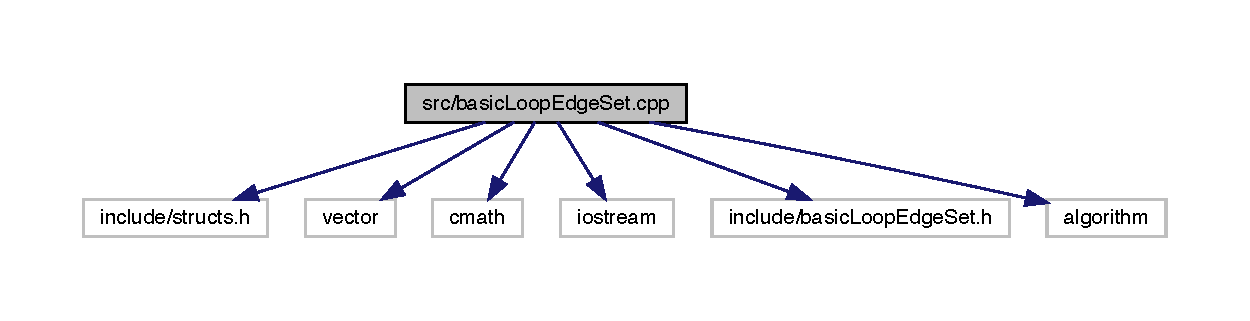
\includegraphics[width=350pt]{basic_loop_edge_set_8cpp__incl}
\end{center}
\end{figure}

\hypertarget{body_loop_8cpp}{}\section{src/body\+Loop.cpp File Reference}
\label{body_loop_8cpp}\index{src/body\+Loop.\+cpp@{src/body\+Loop.\+cpp}}
{\ttfamily \#include $<$vector$>$}\newline
{\ttfamily \#include \char`\"{}include/structs.\+h\char`\"{}}\newline
{\ttfamily \#include \char`\"{}include/face\+Loop.\+h\char`\"{}}\newline
{\ttfamily \#include $<$algorithm$>$}\newline
{\ttfamily \#include \char`\"{}include/body\+Loop.\+h\char`\"{}}\newline
Include dependency graph for body\+Loop.\+cpp\+:
\nopagebreak
\begin{figure}[H]
\begin{center}
\leavevmode
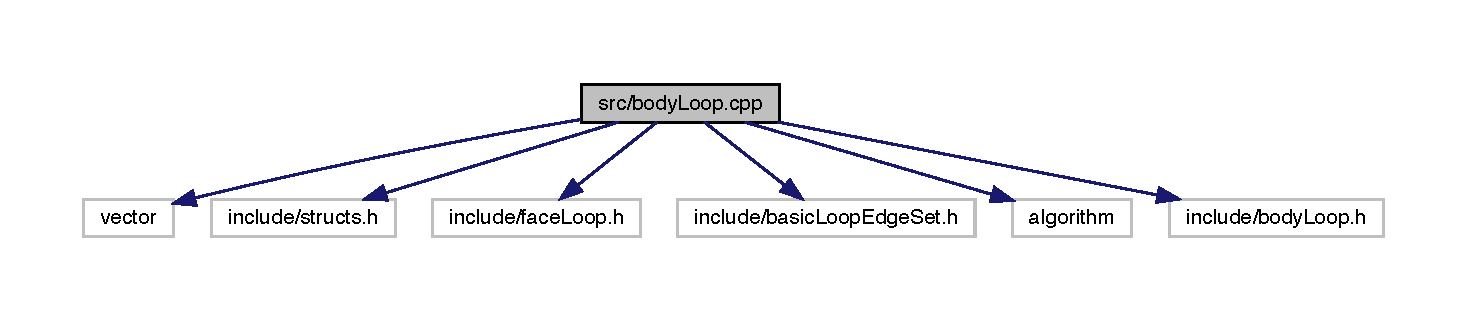
\includegraphics[width=350pt]{body_loop_8cpp__incl}
\end{center}
\end{figure}

\hypertarget{_edge_list2_d_8cpp}{}\section{src/\+Edge\+List2D.cpp File Reference}
\label{_edge_list2_d_8cpp}\index{src/\+Edge\+List2\+D.\+cpp@{src/\+Edge\+List2\+D.\+cpp}}
{\ttfamily \#include $<$iostream$>$}\newline
{\ttfamily \#include \char`\"{}include/structs.\+h\char`\"{}}\newline
{\ttfamily \#include \char`\"{}include/\+Edge\+List2\+D.\+h\char`\"{}}\newline
{\ttfamily \#include $<$algorithm$>$}\newline
Include dependency graph for Edge\+List2\+D.\+cpp\+:
\nopagebreak
\begin{figure}[H]
\begin{center}
\leavevmode
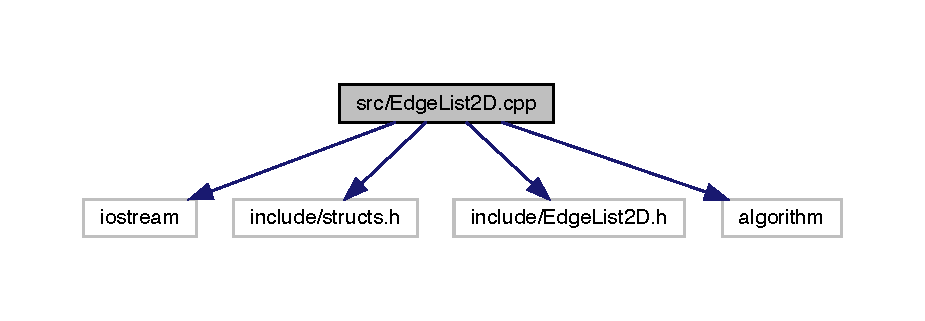
\includegraphics[width=350pt]{_edge_list2_d_8cpp__incl}
\end{center}
\end{figure}

\hypertarget{face_loop_8cpp}{}\section{src/face\+Loop.cpp File Reference}
\label{face_loop_8cpp}\index{src/face\+Loop.\+cpp@{src/face\+Loop.\+cpp}}
{\ttfamily \#include $<$vector$>$}\newline
{\ttfamily \#include \char`\"{}include/structs.\+h\char`\"{}}\newline
{\ttfamily \#include \char`\"{}include/face\+Loop.\+h\char`\"{}}\newline
{\ttfamily \#include \char`\"{}include/basic\+Loop\+Edge\+Set.\+h\char`\"{}}\newline
{\ttfamily \#include \char`\"{}include/general\+Methods.\+h\char`\"{}}\newline
{\ttfamily \#include $<$iostream$>$}\newline
{\ttfamily \#include $<$algorithm$>$}\newline
Include dependency graph for face\+Loop.\+cpp\+:
\nopagebreak
\begin{figure}[H]
\begin{center}
\leavevmode
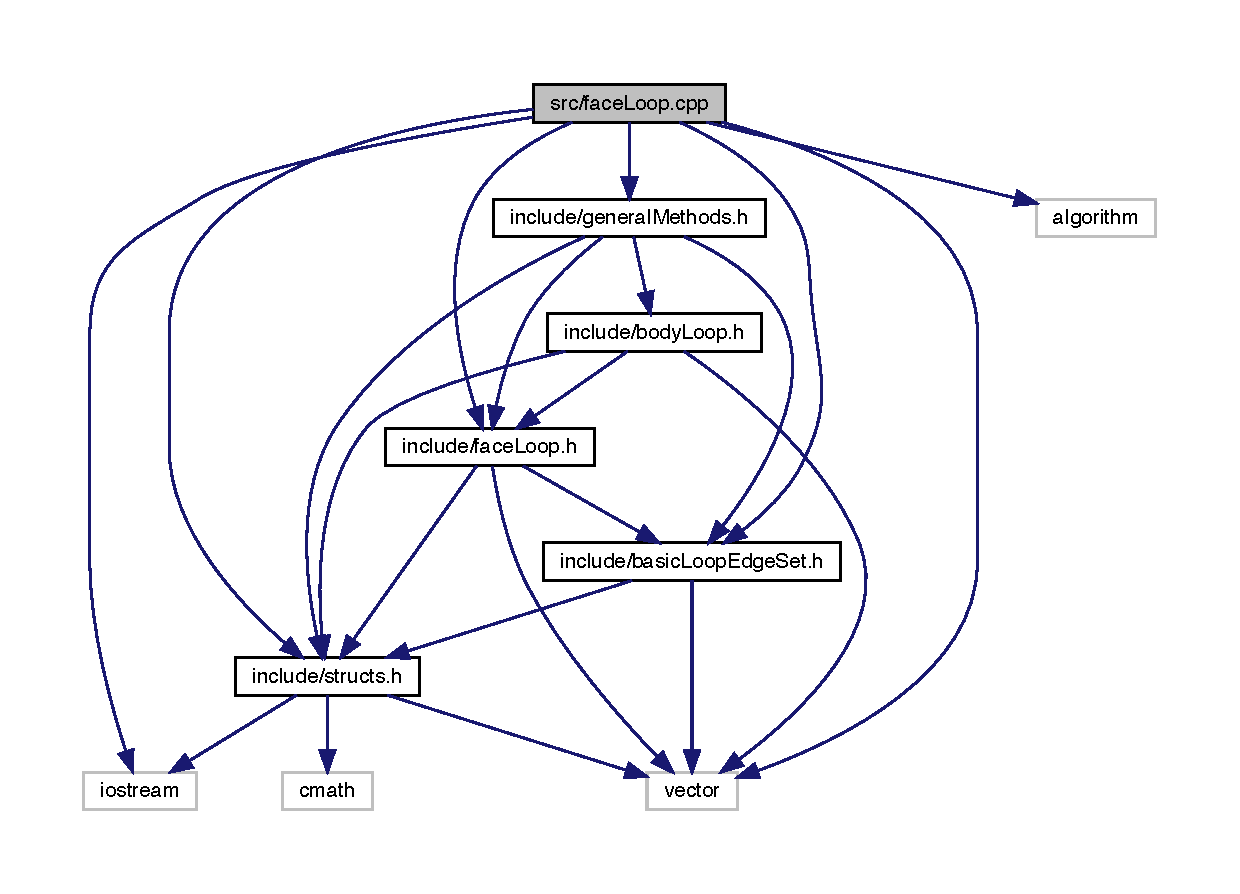
\includegraphics[width=350pt]{face_loop_8cpp__incl}
\end{center}
\end{figure}
\subsection*{Functions}
\begin{DoxyCompactItemize}
\item 
basic\+Loop\+Edge\+Set \mbox{\hyperlink{face_loop_8cpp_aebdb45838a000cabd4e38425b5a2f4d4}{reversebasic\+Loop\+Edge\+Set}} (basic\+Loop\+Edge\+Set bles)
\end{DoxyCompactItemize}


\subsection{Function Documentation}
\mbox{\Hypertarget{face_loop_8cpp_aebdb45838a000cabd4e38425b5a2f4d4}\label{face_loop_8cpp_aebdb45838a000cabd4e38425b5a2f4d4}} 
\index{face\+Loop.\+cpp@{face\+Loop.\+cpp}!reversebasic\+Loop\+Edge\+Set@{reversebasic\+Loop\+Edge\+Set}}
\index{reversebasic\+Loop\+Edge\+Set@{reversebasic\+Loop\+Edge\+Set}!face\+Loop.\+cpp@{face\+Loop.\+cpp}}
\subsubsection{\texorpdfstring{reversebasic\+Loop\+Edge\+Set()}{reversebasicLoopEdgeSet()}}
{\footnotesize\ttfamily basic\+Loop\+Edge\+Set reversebasic\+Loop\+Edge\+Set (\begin{DoxyParamCaption}\item[{basic\+Loop\+Edge\+Set}]{bles }\end{DoxyParamCaption})}



Definition at line 33 of file face\+Loop.\+cpp.

Here is the caller graph for this function\+:
\nopagebreak
\begin{figure}[H]
\begin{center}
\leavevmode
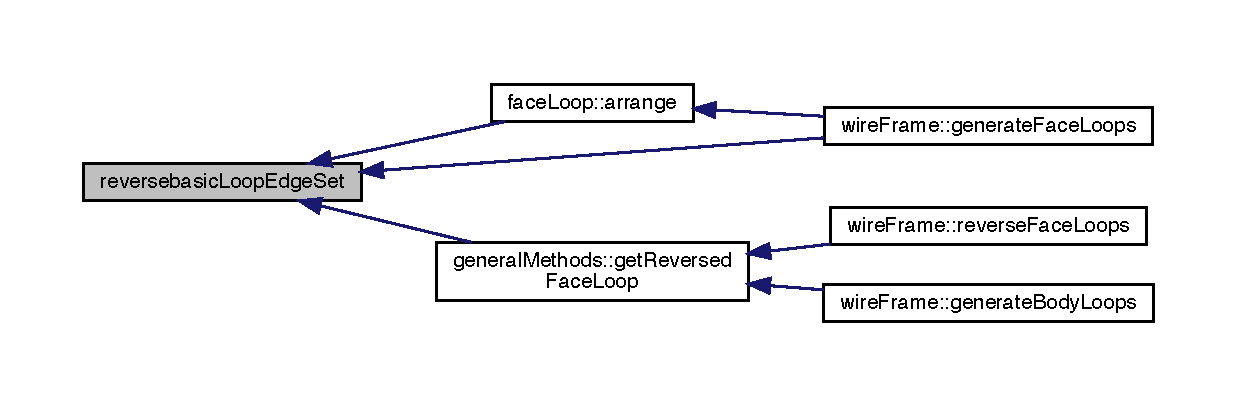
\includegraphics[width=350pt]{face_loop_8cpp_aebdb45838a000cabd4e38425b5a2f4d4_icgraph}
\end{center}
\end{figure}

\hypertarget{general_methods_8cpp}{}\section{src/general\+Methods.cpp File Reference}
\label{general_methods_8cpp}\index{src/general\+Methods.\+cpp@{src/general\+Methods.\+cpp}}
{\ttfamily \#include \char`\"{}include/structs.\+h\char`\"{}}\newline
{\ttfamily \#include \char`\"{}include/basic\+Loop\+Edge\+Set.\+h\char`\"{}}\newline
{\ttfamily \#include \char`\"{}include/face\+Loop.\+h\char`\"{}}\newline
{\ttfamily \#include \char`\"{}include/body\+Loop.\+h\char`\"{}}\newline
{\ttfamily \#include \char`\"{}include/general\+Methods.\+h\char`\"{}}\newline
{\ttfamily \#include $<$math.\+h$>$}\newline
{\ttfamily \#include $<$cstdlib$>$}\newline
{\ttfamily \#include $<$climits$>$}\newline
{\ttfamily \#include $<$iostream$>$}\newline
{\ttfamily \#include $<$cmath$>$}\newline
{\ttfamily \#include $<$algorithm$>$}\newline
Include dependency graph for general\+Methods.\+cpp\+:
\nopagebreak
\begin{figure}[H]
\begin{center}
\leavevmode
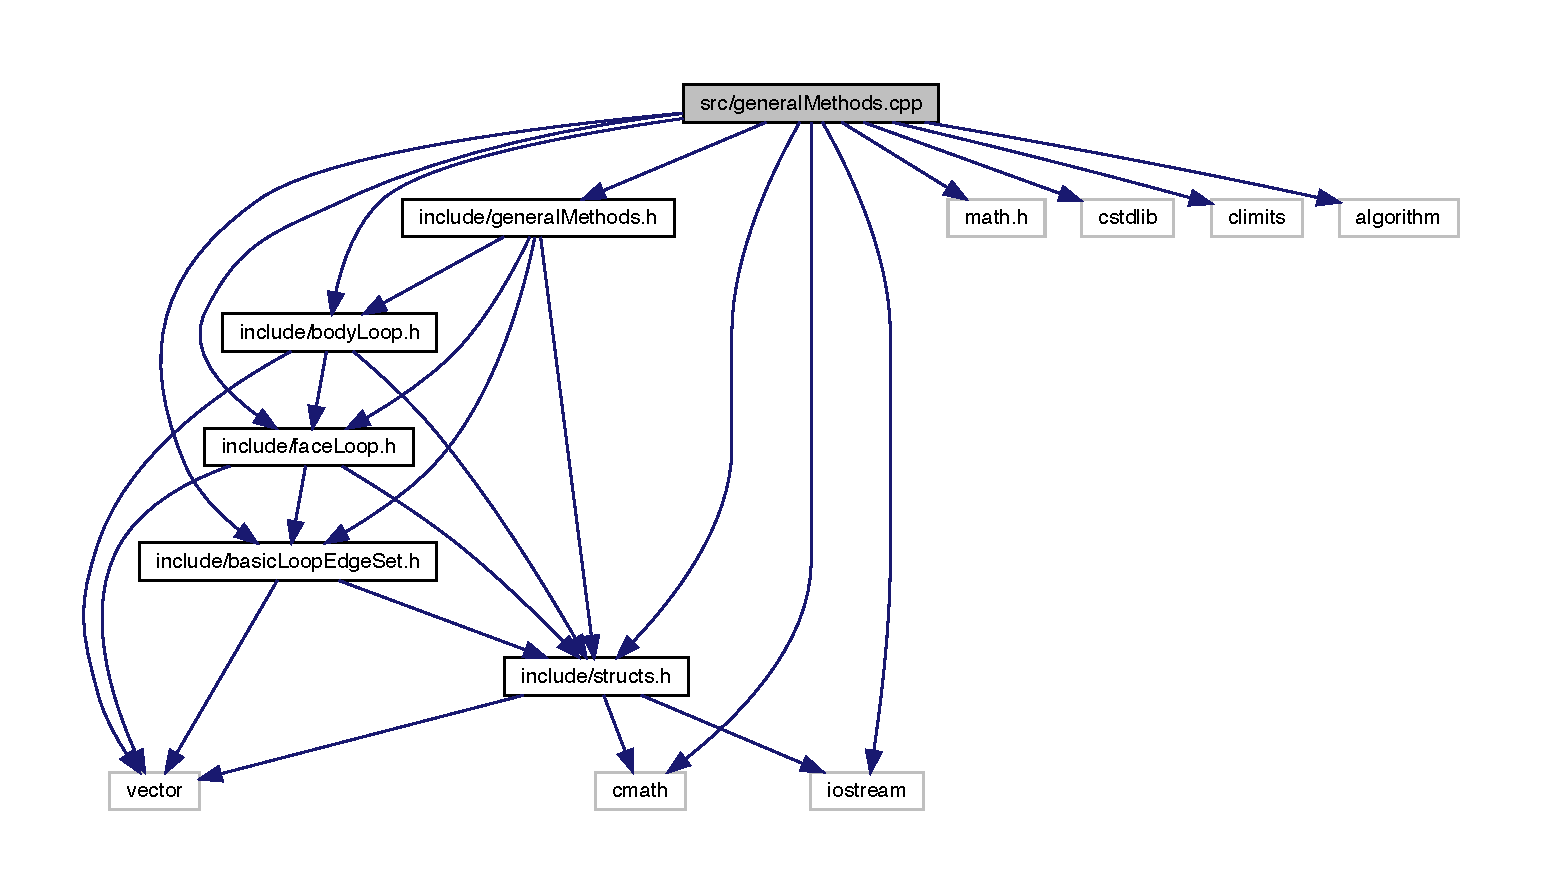
\includegraphics[width=350pt]{general_methods_8cpp__incl}
\end{center}
\end{figure}
\subsection*{Namespaces}
\begin{DoxyCompactItemize}
\item 
 \mbox{\hyperlink{namespacegeneral_methods}{general\+Methods}}
\end{DoxyCompactItemize}
\subsection*{Macros}
\begin{DoxyCompactItemize}
\item 
\#define \mbox{\hyperlink{general_methods_8cpp_a598a3330b3c21701223ee0ca14316eca}{PI}}~3.\+141592653f
\end{DoxyCompactItemize}
\subsection*{Functions}
\begin{DoxyCompactItemize}
\item 
void \mbox{\hyperlink{namespacegeneral_methods_a694306c7472ee1bbfb3c90c0f3d5453a}{general\+Methods\+::print\+Vertex}} (\mbox{\hyperlink{structvertex3_d}{vertex3D}} i)
\begin{DoxyCompactList}\small\item\em print methods \end{DoxyCompactList}\item 
void \mbox{\hyperlink{namespacegeneral_methods_a9cbf7d7c2019f0e2b6f9773b687b50cd}{general\+Methods\+::print\+Vertices\+List}} (vector$<$ \mbox{\hyperlink{structvertex3_d}{vertex3D}} $>$ v)
\item 
void \mbox{\hyperlink{namespacegeneral_methods_af9a1c28dacf89e746b51916fe178ce1a}{general\+Methods\+::print\+Edge}} (\mbox{\hyperlink{structedge3_d}{edge3D}} i)
\item 
void \mbox{\hyperlink{namespacegeneral_methods_ab6b6f8a5d92b39ead6c97ec0917b75a4}{general\+Methods\+::print\+Edge\+List}} (vector$<$ \mbox{\hyperlink{structedge3_d}{edge3D}} $>$ e)
\item 
void \mbox{\hyperlink{namespacegeneral_methods_a3474d24f9f545407bb5f73250a5e19d7}{general\+Methods\+::print\+Plane}} (\mbox{\hyperlink{structplane}{plane}} p)
\item 
void \mbox{\hyperlink{namespacegeneral_methods_aa7c9b8abc94ae6b08d2cf083a08eaf21}{general\+Methods\+::print\+Planes}} (vector$<$ \mbox{\hyperlink{structplane}{plane}} $>$ p)
\item 
void \mbox{\hyperlink{namespacegeneral_methods_a60a9e0ba058824389fc703dc2dbbb7e3}{general\+Methods\+::print\+V\+E\+List}} (\mbox{\hyperlink{structvertex_edge_list}{vertex\+Edge\+List}} ve\+List)
\item 
void \mbox{\hyperlink{namespacegeneral_methods_adc8e104a2f2ed35a22be9a68051ec38d}{general\+Methods\+::printplane\+V\+EL}} (\mbox{\hyperlink{structplane_v_e_l}{plane\+V\+EL}} p)
\item 
bool \mbox{\hyperlink{namespacegeneral_methods_afc8f20af710f8dc24af591015acc1403}{general\+Methods\+::compare\+Pairs}} (\mbox{\hyperlink{structvertex_edge_pair}{vertex\+Edge\+Pair}} pair1, \mbox{\hyperlink{structvertex_edge_pair}{vertex\+Edge\+Pair}} pair2)
\item 
std\+::vector$<$ \mbox{\hyperlink{structvertex3_d}{vertex3D}} $>$ \mbox{\hyperlink{namespacegeneral_methods_ace3487740f3b46dce9e0357366abf9ed}{general\+Methods\+::sort\+Vertices}} (std\+::vector$<$ \mbox{\hyperlink{structvertex3_d}{vertex3D}} $>$ V, \mbox{\hyperlink{structedge3_d}{edge3D}} e)
\item 
bool \mbox{\hyperlink{namespacegeneral_methods_aa7662b2bcff30f8983da23da5edfc766}{general\+Methods\+::check\+Overlap\+Collinear}} (\mbox{\hyperlink{structedge3_d}{edge3D}} e1, \mbox{\hyperlink{structedge3_d}{edge3D}} e2)
\item 
bool \mbox{\hyperlink{namespacegeneral_methods_a508d15a0c76920dc4f98cf8da254f9c4}{general\+Methods\+::check\+Coplanar}} (\mbox{\hyperlink{structedge3_d}{edge3D}} e1, \mbox{\hyperlink{structedge3_d}{edge3D}} e2, \mbox{\hyperlink{structedge3_d}{edge3D}} e3)
\item 
\mbox{\hyperlink{structplane}{plane}} \mbox{\hyperlink{namespacegeneral_methods_a06d99f1b292d29dbdbe4734847c8d2ee}{general\+Methods\+::make\+Plane}} (\mbox{\hyperlink{structedge3_d}{edge3D}} e1, \mbox{\hyperlink{structedge3_d}{edge3D}} e2)
\item 
bool \mbox{\hyperlink{namespacegeneral_methods_a3c49599a5ba8f2c41f2ef542bde19765}{general\+Methods\+::plane\+Equal}} (\mbox{\hyperlink{structplane}{plane}} p1, \mbox{\hyperlink{structplane}{plane}} p2)
\item 
std\+::vector$<$ \mbox{\hyperlink{structplane}{plane}} $>$ \mbox{\hyperlink{namespacegeneral_methods_a13072e8b14fcea9ae253085569062158}{general\+Methods\+::remove\+Duplicate}} (std\+::vector$<$ \mbox{\hyperlink{structplane}{plane}} $>$ v)
\item 
float \mbox{\hyperlink{namespacegeneral_methods_a3bc88a001e751ad419e87bf3795ca02b}{general\+Methods\+::find\+Distance\+Between\+Planes}} (\mbox{\hyperlink{structplane}{plane}} p, \mbox{\hyperlink{structplane}{plane}} q)
\item 
bool \mbox{\hyperlink{namespacegeneral_methods_a330682bb45234d8de5228a7607d493d2}{general\+Methods\+::if\+Vertex\+On\+Plane}} (\mbox{\hyperlink{structplane}{plane}} p, \mbox{\hyperlink{structvertex3_d}{vertex3D}} v)
\item 
bool \mbox{\hyperlink{namespacegeneral_methods_a21d2e8c181e8cac3762d9ca1871d2168}{general\+Methods\+::if\+Edge\+On\+Plane}} (\mbox{\hyperlink{structplane}{plane}} p, \mbox{\hyperlink{structedge3_d}{edge3D}} e)
\item 
std\+::vector$<$ \mbox{\hyperlink{structedge3_d}{edge3D}} $>$ \mbox{\hyperlink{namespacegeneral_methods_a9bff72be73e4d6faec798a23b8f28cb9}{general\+Methods\+::find\+Edges\+On\+Plane}} (\mbox{\hyperlink{structplane}{plane}} p, std\+::vector$<$ \mbox{\hyperlink{structedge3_d}{edge3D}} $>$ e\+List)
\item 
std\+::vector$<$ \mbox{\hyperlink{structvertex3_d}{vertex3D}} $>$ \mbox{\hyperlink{namespacegeneral_methods_aa0669678cf59876e3249ddce7a0d1ce3}{general\+Methods\+::find\+Vertices\+On\+Plane}} (\mbox{\hyperlink{structplane}{plane}} p, std\+::vector$<$ \mbox{\hyperlink{structvertex3_d}{vertex3D}} $>$ eop)
\item 
bool \mbox{\hyperlink{namespacegeneral_methods_ab4e1b4b0a8b5b7697adddbb27950e639}{general\+Methods\+::check\+Hidden}} (\mbox{\hyperlink{structplane}{plane}} p, \mbox{\hyperlink{structedge3_d}{edge3D}} e, float \mbox{\hyperlink{structdirection}{direction}}\mbox{[}$\,$\mbox{]})
\item 
bool \mbox{\hyperlink{namespacegeneral_methods_a557bf2257d6658862b42124035aa9588}{general\+Methods\+::on\+Segment}} (\mbox{\hyperlink{structvertex3_d}{vertex3D}} v, \mbox{\hyperlink{structedge3_d}{edge3D}} edge)
\item 
int \mbox{\hyperlink{namespacegeneral_methods_a7bfbfb2a02328d76e70f66fedd57c4ef}{general\+Methods\+::orientation}} (\mbox{\hyperlink{structvertex3_d}{vertex3D}} p, \mbox{\hyperlink{structvertex3_d}{vertex3D}} q, \mbox{\hyperlink{structvertex3_d}{vertex3D}} r, \mbox{\hyperlink{structplane}{plane}} s)
\item 
bool \mbox{\hyperlink{namespacegeneral_methods_a56efd049c58aae30a7b0caf39beab615}{general\+Methods\+::do\+Intersect}} (\mbox{\hyperlink{structvertex3_d}{vertex3D}} p1, \mbox{\hyperlink{structvertex3_d}{vertex3D}} q1, \mbox{\hyperlink{structvertex3_d}{vertex3D}} p2, \mbox{\hyperlink{structvertex3_d}{vertex3D}} q2, \mbox{\hyperlink{structplane}{plane}} p)
\item 
bool \mbox{\hyperlink{namespacegeneral_methods_a27b7ed292415027c495942147e8856b7}{general\+Methods\+::is\+Inside}} (std\+::vector$<$ \mbox{\hyperlink{structvertex3_d}{vertex3D}} $>$ polygon, int n, \mbox{\hyperlink{structvertex3_d}{vertex3D}} p, \mbox{\hyperlink{structedge3_d}{edge3D}} ref\+Edge, \mbox{\hyperlink{structplane}{plane}} q)
\item 
int \mbox{\hyperlink{namespacegeneral_methods_a2bb810600ec90ec064ea8496ee0ab862}{general\+Methods\+::check\+Confinement}} (\mbox{\hyperlink{classbasic_loop_edge_set}{basic\+Loop\+Edge\+Set}} fl1, \mbox{\hyperlink{classbasic_loop_edge_set}{basic\+Loop\+Edge\+Set}} fl2, \mbox{\hyperlink{structplane}{plane}} p)
\item 
float $\ast$ \mbox{\hyperlink{namespacegeneral_methods_a0bd9c59442b6f9c7fd3ae00832ee30df}{general\+Methods\+::get\+Alpha\+And\+Direction}} (\mbox{\hyperlink{classface_loop}{face\+Loop}} flk, \mbox{\hyperlink{classface_loop}{face\+Loop}} fls, \mbox{\hyperlink{structedge3_d}{edge3D}} reference\+Edge)
\item 
\mbox{\hyperlink{classface_loop}{face\+Loop}} \mbox{\hyperlink{namespacegeneral_methods_afe4087e253b318326a0a1578d34b42ca}{general\+Methods\+::get\+Reversed\+Face\+Loop}} (\mbox{\hyperlink{classface_loop}{face\+Loop}} faceloop)
\end{DoxyCompactItemize}


\subsection{Macro Definition Documentation}
\mbox{\Hypertarget{general_methods_8cpp_a598a3330b3c21701223ee0ca14316eca}\label{general_methods_8cpp_a598a3330b3c21701223ee0ca14316eca}} 
\index{general\+Methods.\+cpp@{general\+Methods.\+cpp}!PI@{PI}}
\index{PI@{PI}!general\+Methods.\+cpp@{general\+Methods.\+cpp}}
\subsubsection{\texorpdfstring{PI}{PI}}
{\footnotesize\ttfamily \#define PI~3.\+141592653f}



Definition at line 15 of file general\+Methods.\+cpp.


\hypertarget{main_8cpp}{}\section{src/main.cpp File Reference}
\label{main_8cpp}\index{src/main.\+cpp@{src/main.\+cpp}}
{\ttfamily \#include \char`\"{}include/selection.\+h\char`\"{}}\newline
{\ttfamily \#include $<$Q\+Application$>$}\newline
Include dependency graph for main.\+cpp\+:
\nopagebreak
\begin{figure}[H]
\begin{center}
\leavevmode
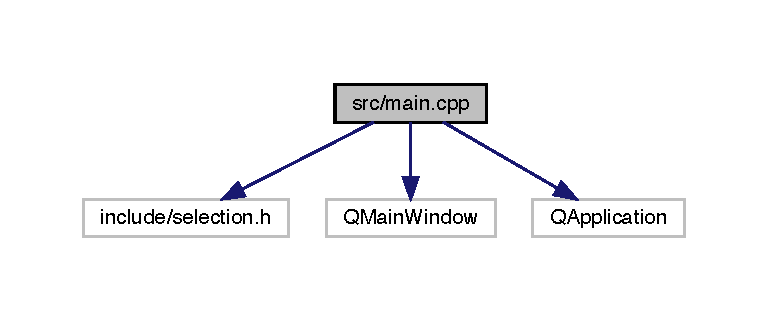
\includegraphics[width=350pt]{main_8cpp__incl}
\end{center}
\end{figure}
\subsection*{Functions}
\begin{DoxyCompactItemize}
\item 
int \mbox{\hyperlink{main_8cpp_a0ddf1224851353fc92bfbff6f499fa97}{main}} (int argc, char $\ast$argv\mbox{[}$\,$\mbox{]})
\end{DoxyCompactItemize}


\subsection{Function Documentation}
\mbox{\Hypertarget{main_8cpp_a0ddf1224851353fc92bfbff6f499fa97}\label{main_8cpp_a0ddf1224851353fc92bfbff6f499fa97}} 
\index{main.\+cpp@{main.\+cpp}!main@{main}}
\index{main@{main}!main.\+cpp@{main.\+cpp}}
\subsubsection{\texorpdfstring{main()}{main()}}
{\footnotesize\ttfamily int main (\begin{DoxyParamCaption}\item[{int}]{argc,  }\item[{char $\ast$}]{argv\mbox{[}$\,$\mbox{]} }\end{DoxyParamCaption})}



Definition at line 386 of file main.\+cpp.


\hypertarget{mainwindow_8cpp}{}\section{src/mainwindow.cpp File Reference}
\label{mainwindow_8cpp}\index{src/mainwindow.\+cpp@{src/mainwindow.\+cpp}}
{\ttfamily \#include \char`\"{}include/mainwindow.\+h\char`\"{}}\newline
{\ttfamily \#include \char`\"{}ui\+\_\+mainwindow.\+h\char`\"{}}\newline
{\ttfamily \#include $<$Q\+File\+Dialog$>$}\newline
{\ttfamily \#include $<$Q\+Message\+Box$>$}\newline
Include dependency graph for mainwindow.\+cpp\+:
\nopagebreak
\begin{figure}[H]
\begin{center}
\leavevmode
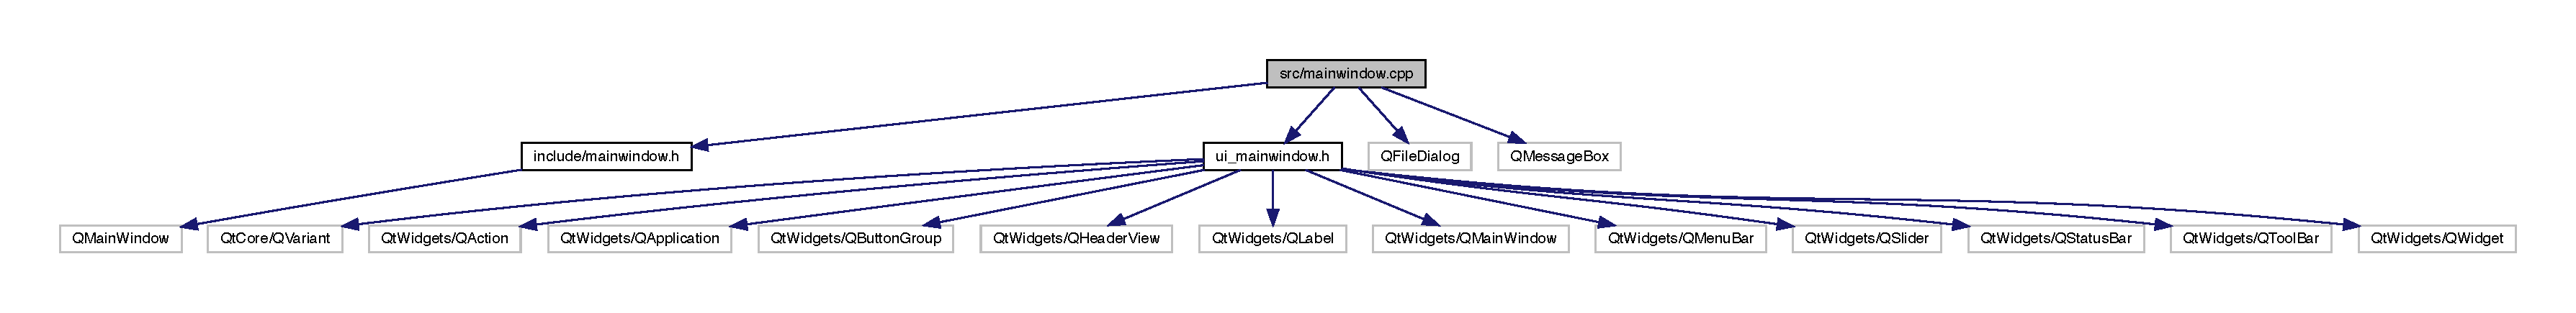
\includegraphics[width=350pt]{mainwindow_8cpp__incl}
\end{center}
\end{figure}

\hypertarget{moc__mainwindow_8cpp}{}\section{src/moc\+\_\+mainwindow.cpp File Reference}
\label{moc__mainwindow_8cpp}\index{src/moc\+\_\+mainwindow.\+cpp@{src/moc\+\_\+mainwindow.\+cpp}}
{\ttfamily \#include \char`\"{}include/mainwindow.\+h\char`\"{}}\newline
{\ttfamily \#include $<$Qt\+Core/qbytearray.\+h$>$}\newline
{\ttfamily \#include $<$Qt\+Core/qmetatype.\+h$>$}\newline
Include dependency graph for moc\+\_\+mainwindow.\+cpp\+:
\nopagebreak
\begin{figure}[H]
\begin{center}
\leavevmode
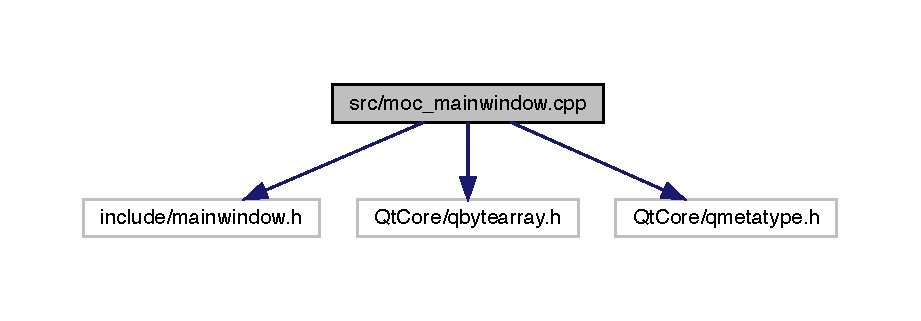
\includegraphics[width=350pt]{moc__mainwindow_8cpp__incl}
\end{center}
\end{figure}
\subsection*{Classes}
\begin{DoxyCompactItemize}
\item 
struct \mbox{\hyperlink{structqt__meta__stringdata___main_window__t}{qt\+\_\+meta\+\_\+stringdata\+\_\+\+Main\+Window\+\_\+t}}
\end{DoxyCompactItemize}
\subsection*{Macros}
\begin{DoxyCompactItemize}
\item 
\#define \mbox{\hyperlink{moc__mainwindow_8cpp_a75bb9482d242cde0a06c9dbdc6b83abe}{Q\+T\+\_\+\+M\+O\+C\+\_\+\+L\+I\+T\+E\+R\+AL}}(idx,  ofs,  len)
\end{DoxyCompactItemize}


\subsection{Macro Definition Documentation}
\mbox{\Hypertarget{moc__mainwindow_8cpp_a75bb9482d242cde0a06c9dbdc6b83abe}\label{moc__mainwindow_8cpp_a75bb9482d242cde0a06c9dbdc6b83abe}} 
\index{moc\+\_\+mainwindow.\+cpp@{moc\+\_\+mainwindow.\+cpp}!Q\+T\+\_\+\+M\+O\+C\+\_\+\+L\+I\+T\+E\+R\+AL@{Q\+T\+\_\+\+M\+O\+C\+\_\+\+L\+I\+T\+E\+R\+AL}}
\index{Q\+T\+\_\+\+M\+O\+C\+\_\+\+L\+I\+T\+E\+R\+AL@{Q\+T\+\_\+\+M\+O\+C\+\_\+\+L\+I\+T\+E\+R\+AL}!moc\+\_\+mainwindow.\+cpp@{moc\+\_\+mainwindow.\+cpp}}
\subsubsection{\texorpdfstring{Q\+T\+\_\+\+M\+O\+C\+\_\+\+L\+I\+T\+E\+R\+AL}{QT\_MOC\_LITERAL}}
{\footnotesize\ttfamily \#define Q\+T\+\_\+\+M\+O\+C\+\_\+\+L\+I\+T\+E\+R\+AL(\begin{DoxyParamCaption}\item[{}]{idx,  }\item[{}]{ofs,  }\item[{}]{len }\end{DoxyParamCaption})}

{\bfseries Value\+:}
\begin{DoxyCode}
Q\_STATIC\_BYTE\_ARRAY\_DATA\_HEADER\_INITIALIZER\_WITH\_OFFSET(len, \(\backslash\)
    qptrdiff(offsetof(\mbox{\hyperlink{structqt__meta__stringdata___main_window__t}{qt\_meta\_stringdata\_MainWindow\_t}}, stringdata0) + ofs \(\backslash\)
        - idx * \textcolor{keyword}{sizeof}(QByteArrayData)) \(\backslash\)
    )
\end{DoxyCode}


Definition at line 25 of file moc\+\_\+mainwindow.\+cpp.


\hypertarget{moc__options_8cpp}{}\section{src/moc\+\_\+options.cpp File Reference}
\label{moc__options_8cpp}\index{src/moc\+\_\+options.\+cpp@{src/moc\+\_\+options.\+cpp}}
{\ttfamily \#include \char`\"{}include/options.\+h\char`\"{}}\newline
{\ttfamily \#include $<$Qt\+Core/qbytearray.\+h$>$}\newline
{\ttfamily \#include $<$Qt\+Core/qmetatype.\+h$>$}\newline
Include dependency graph for moc\+\_\+options.\+cpp\+:
\nopagebreak
\begin{figure}[H]
\begin{center}
\leavevmode
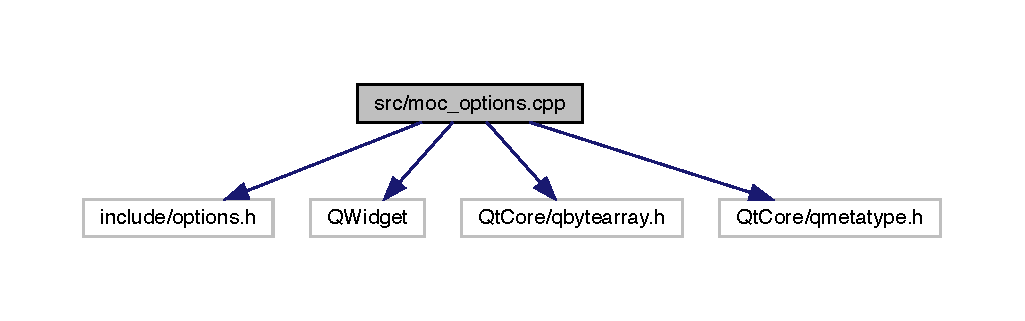
\includegraphics[width=350pt]{moc__options_8cpp__incl}
\end{center}
\end{figure}
\subsection*{Classes}
\begin{DoxyCompactItemize}
\item 
struct \mbox{\hyperlink{structqt__meta__stringdata___options__t}{qt\+\_\+meta\+\_\+stringdata\+\_\+\+Options\+\_\+t}}
\end{DoxyCompactItemize}
\subsection*{Macros}
\begin{DoxyCompactItemize}
\item 
\#define \mbox{\hyperlink{moc__options_8cpp_a75bb9482d242cde0a06c9dbdc6b83abe}{Q\+T\+\_\+\+M\+O\+C\+\_\+\+L\+I\+T\+E\+R\+AL}}(idx,  ofs,  len)
\end{DoxyCompactItemize}


\subsection{Macro Definition Documentation}
\mbox{\Hypertarget{moc__options_8cpp_a75bb9482d242cde0a06c9dbdc6b83abe}\label{moc__options_8cpp_a75bb9482d242cde0a06c9dbdc6b83abe}} 
\index{moc\+\_\+options.\+cpp@{moc\+\_\+options.\+cpp}!Q\+T\+\_\+\+M\+O\+C\+\_\+\+L\+I\+T\+E\+R\+AL@{Q\+T\+\_\+\+M\+O\+C\+\_\+\+L\+I\+T\+E\+R\+AL}}
\index{Q\+T\+\_\+\+M\+O\+C\+\_\+\+L\+I\+T\+E\+R\+AL@{Q\+T\+\_\+\+M\+O\+C\+\_\+\+L\+I\+T\+E\+R\+AL}!moc\+\_\+options.\+cpp@{moc\+\_\+options.\+cpp}}
\subsubsection{\texorpdfstring{Q\+T\+\_\+\+M\+O\+C\+\_\+\+L\+I\+T\+E\+R\+AL}{QT\_MOC\_LITERAL}}
{\footnotesize\ttfamily \#define Q\+T\+\_\+\+M\+O\+C\+\_\+\+L\+I\+T\+E\+R\+AL(\begin{DoxyParamCaption}\item[{}]{idx,  }\item[{}]{ofs,  }\item[{}]{len }\end{DoxyParamCaption})}

{\bfseries Value\+:}
\begin{DoxyCode}
Q\_STATIC\_BYTE\_ARRAY\_DATA\_HEADER\_INITIALIZER\_WITH\_OFFSET(len, \(\backslash\)
    qptrdiff(offsetof(\mbox{\hyperlink{structqt__meta__stringdata___options__t}{qt\_meta\_stringdata\_Options\_t}}, stringdata0) + ofs \(\backslash\)
        - idx * \textcolor{keyword}{sizeof}(QByteArrayData)) \(\backslash\)
    )
\end{DoxyCode}


Definition at line 25 of file moc\+\_\+options.\+cpp.


\hypertarget{moc__selection_8cpp}{}\section{src/moc\+\_\+selection.cpp File Reference}
\label{moc__selection_8cpp}\index{src/moc\+\_\+selection.\+cpp@{src/moc\+\_\+selection.\+cpp}}
{\ttfamily \#include \char`\"{}include/selection.\+h\char`\"{}}\newline
{\ttfamily \#include $<$Qt\+Core/qbytearray.\+h$>$}\newline
{\ttfamily \#include $<$Qt\+Core/qmetatype.\+h$>$}\newline
Include dependency graph for moc\+\_\+selection.\+cpp\+:
\nopagebreak
\begin{figure}[H]
\begin{center}
\leavevmode
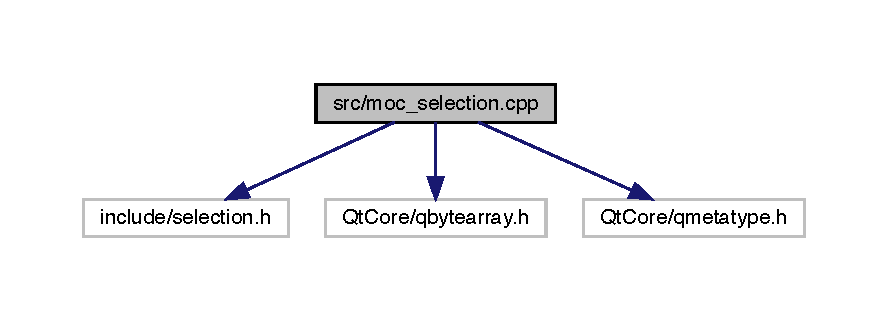
\includegraphics[width=350pt]{moc__selection_8cpp__incl}
\end{center}
\end{figure}
\subsection*{Classes}
\begin{DoxyCompactItemize}
\item 
struct \mbox{\hyperlink{structqt__meta__stringdata___selection__t}{qt\+\_\+meta\+\_\+stringdata\+\_\+\+Selection\+\_\+t}}
\end{DoxyCompactItemize}
\subsection*{Macros}
\begin{DoxyCompactItemize}
\item 
\#define \mbox{\hyperlink{moc__selection_8cpp_a75bb9482d242cde0a06c9dbdc6b83abe}{Q\+T\+\_\+\+M\+O\+C\+\_\+\+L\+I\+T\+E\+R\+AL}}(idx,  ofs,  len)
\end{DoxyCompactItemize}


\subsection{Macro Definition Documentation}
\mbox{\Hypertarget{moc__selection_8cpp_a75bb9482d242cde0a06c9dbdc6b83abe}\label{moc__selection_8cpp_a75bb9482d242cde0a06c9dbdc6b83abe}} 
\index{moc\+\_\+selection.\+cpp@{moc\+\_\+selection.\+cpp}!Q\+T\+\_\+\+M\+O\+C\+\_\+\+L\+I\+T\+E\+R\+AL@{Q\+T\+\_\+\+M\+O\+C\+\_\+\+L\+I\+T\+E\+R\+AL}}
\index{Q\+T\+\_\+\+M\+O\+C\+\_\+\+L\+I\+T\+E\+R\+AL@{Q\+T\+\_\+\+M\+O\+C\+\_\+\+L\+I\+T\+E\+R\+AL}!moc\+\_\+selection.\+cpp@{moc\+\_\+selection.\+cpp}}
\subsubsection{\texorpdfstring{Q\+T\+\_\+\+M\+O\+C\+\_\+\+L\+I\+T\+E\+R\+AL}{QT\_MOC\_LITERAL}}
{\footnotesize\ttfamily \#define Q\+T\+\_\+\+M\+O\+C\+\_\+\+L\+I\+T\+E\+R\+AL(\begin{DoxyParamCaption}\item[{}]{idx,  }\item[{}]{ofs,  }\item[{}]{len }\end{DoxyParamCaption})}

{\bfseries Value\+:}
\begin{DoxyCode}
Q\_STATIC\_BYTE\_ARRAY\_DATA\_HEADER\_INITIALIZER\_WITH\_OFFSET(len, \(\backslash\)
    qptrdiff(offsetof(\mbox{\hyperlink{structqt__meta__stringdata___selection__t}{qt\_meta\_stringdata\_Selection\_t}}, stringdata0) + ofs \(\backslash\)
        - idx * \textcolor{keyword}{sizeof}(QByteArrayData)) \(\backslash\)
    )
\end{DoxyCode}


Definition at line 25 of file moc\+\_\+selection.\+cpp.


\hypertarget{moc__showprojections_8cpp}{}\section{src/moc\+\_\+showprojections.cpp File Reference}
\label{moc__showprojections_8cpp}\index{src/moc\+\_\+showprojections.\+cpp@{src/moc\+\_\+showprojections.\+cpp}}
{\ttfamily \#include \char`\"{}include/showprojections.\+h\char`\"{}}\newline
{\ttfamily \#include $<$Qt\+Core/qbytearray.\+h$>$}\newline
{\ttfamily \#include $<$Qt\+Core/qmetatype.\+h$>$}\newline
Include dependency graph for moc\+\_\+showprojections.\+cpp\+:
\nopagebreak
\begin{figure}[H]
\begin{center}
\leavevmode
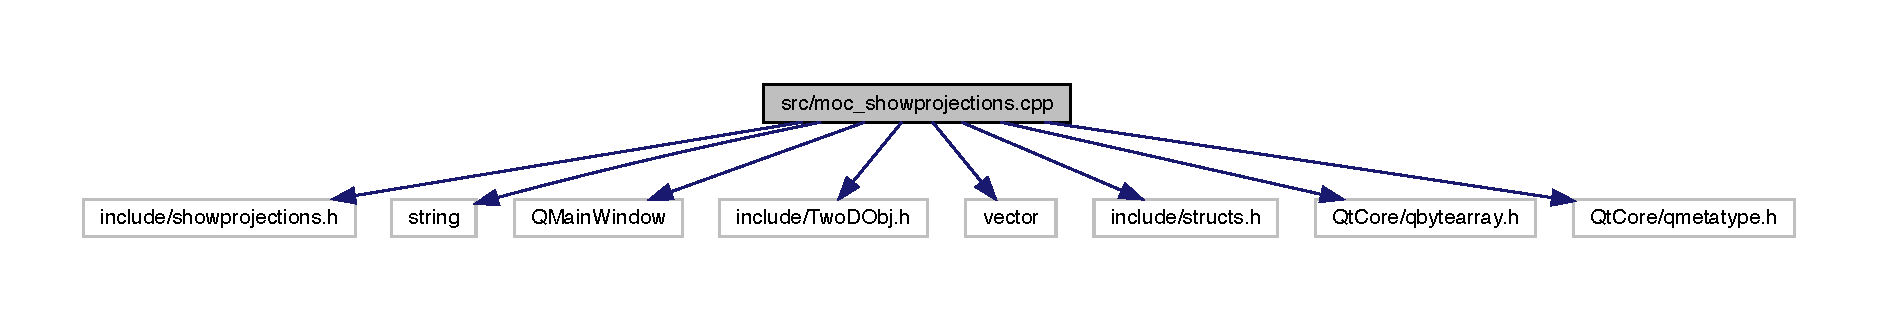
\includegraphics[width=350pt]{moc__showprojections_8cpp__incl}
\end{center}
\end{figure}
\subsection*{Classes}
\begin{DoxyCompactItemize}
\item 
struct \mbox{\hyperlink{structqt__meta__stringdata___show_projections__t}{qt\+\_\+meta\+\_\+stringdata\+\_\+\+Show\+Projections\+\_\+t}}
\end{DoxyCompactItemize}
\subsection*{Macros}
\begin{DoxyCompactItemize}
\item 
\#define \mbox{\hyperlink{moc__showprojections_8cpp_a75bb9482d242cde0a06c9dbdc6b83abe}{Q\+T\+\_\+\+M\+O\+C\+\_\+\+L\+I\+T\+E\+R\+AL}}(idx,  ofs,  len)
\end{DoxyCompactItemize}


\subsection{Macro Definition Documentation}
\mbox{\Hypertarget{moc__showprojections_8cpp_a75bb9482d242cde0a06c9dbdc6b83abe}\label{moc__showprojections_8cpp_a75bb9482d242cde0a06c9dbdc6b83abe}} 
\index{moc\+\_\+showprojections.\+cpp@{moc\+\_\+showprojections.\+cpp}!Q\+T\+\_\+\+M\+O\+C\+\_\+\+L\+I\+T\+E\+R\+AL@{Q\+T\+\_\+\+M\+O\+C\+\_\+\+L\+I\+T\+E\+R\+AL}}
\index{Q\+T\+\_\+\+M\+O\+C\+\_\+\+L\+I\+T\+E\+R\+AL@{Q\+T\+\_\+\+M\+O\+C\+\_\+\+L\+I\+T\+E\+R\+AL}!moc\+\_\+showprojections.\+cpp@{moc\+\_\+showprojections.\+cpp}}
\subsubsection{\texorpdfstring{Q\+T\+\_\+\+M\+O\+C\+\_\+\+L\+I\+T\+E\+R\+AL}{QT\_MOC\_LITERAL}}
{\footnotesize\ttfamily \#define Q\+T\+\_\+\+M\+O\+C\+\_\+\+L\+I\+T\+E\+R\+AL(\begin{DoxyParamCaption}\item[{}]{idx,  }\item[{}]{ofs,  }\item[{}]{len }\end{DoxyParamCaption})}

{\bfseries Value\+:}
\begin{DoxyCode}
Q\_STATIC\_BYTE\_ARRAY\_DATA\_HEADER\_INITIALIZER\_WITH\_OFFSET(len, \(\backslash\)
    qptrdiff(offsetof(\mbox{\hyperlink{structqt__meta__stringdata___show_projections__t}{qt\_meta\_stringdata\_ShowProjections\_t}}, stringdata0
      ) + ofs \(\backslash\)
        - idx * \textcolor{keyword}{sizeof}(QByteArrayData)) \(\backslash\)
    )
\end{DoxyCode}


Definition at line 25 of file moc\+\_\+showprojections.\+cpp.


\hypertarget{options_8cpp}{}\section{src/options.cpp File Reference}
\label{options_8cpp}\index{src/options.\+cpp@{src/options.\+cpp}}
{\ttfamily \#include \char`\"{}include/options.\+h\char`\"{}}\newline
Include dependency graph for options.\+cpp\+:
\nopagebreak
\begin{figure}[H]
\begin{center}
\leavevmode
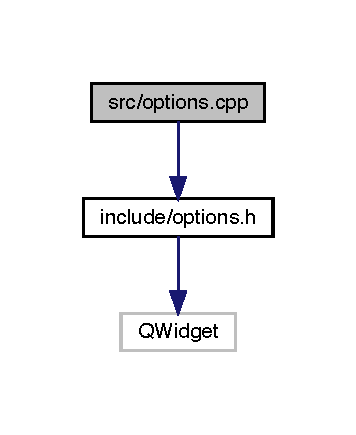
\includegraphics[width=171pt]{options_8cpp__incl}
\end{center}
\end{figure}

\hypertarget{_plane_8cpp}{}\section{src/\+Plane.cpp File Reference}
\label{_plane_8cpp}\index{src/\+Plane.\+cpp@{src/\+Plane.\+cpp}}
{\ttfamily \#include \char`\"{}include/structs.\+h\char`\"{}}\newline
{\ttfamily \#include \char`\"{}include/\+Plane.\+h\char`\"{}}\newline
{\ttfamily \#include $<$cmath$>$}\newline
{\ttfamily \#include $<$algorithm$>$}\newline
Include dependency graph for Plane.\+cpp\+:
\nopagebreak
\begin{figure}[H]
\begin{center}
\leavevmode
\includegraphics[width=350pt]{_plane_8cpp__incl}
\end{center}
\end{figure}
\subsection*{Macros}
\begin{DoxyCompactItemize}
\item 
\#define \mbox{\hyperlink{_plane_8cpp_a598a3330b3c21701223ee0ca14316eca}{PI}}~3.\+14159265
\end{DoxyCompactItemize}
\subsection*{Functions}
\begin{DoxyCompactItemize}
\item 
float \mbox{\hyperlink{_plane_8cpp_a41b3f23bbae2d530aafc33c3d82b19d2}{find\+Angle}} (edge3D ref\+Edge, edge3D other\+Edge, vertex3D ref\+Vertex, plane p)
\item 
bool \mbox{\hyperlink{_plane_8cpp_ab32167b9c5f90ae9269be5b7ce973682}{compare\+Triplets}} (edge\+Vertex\+Triplet t1, edge\+Vertex\+Triplet t2)
\end{DoxyCompactItemize}


\subsection{Macro Definition Documentation}
\mbox{\Hypertarget{_plane_8cpp_a598a3330b3c21701223ee0ca14316eca}\label{_plane_8cpp_a598a3330b3c21701223ee0ca14316eca}} 
\index{Plane.\+cpp@{Plane.\+cpp}!PI@{PI}}
\index{PI@{PI}!Plane.\+cpp@{Plane.\+cpp}}
\subsubsection{\texorpdfstring{PI}{PI}}
{\footnotesize\ttfamily \#define PI~3.\+14159265}



Definition at line 8 of file Plane.\+cpp.



\subsection{Function Documentation}
\mbox{\Hypertarget{_plane_8cpp_ab32167b9c5f90ae9269be5b7ce973682}\label{_plane_8cpp_ab32167b9c5f90ae9269be5b7ce973682}} 
\index{Plane.\+cpp@{Plane.\+cpp}!compare\+Triplets@{compare\+Triplets}}
\index{compare\+Triplets@{compare\+Triplets}!Plane.\+cpp@{Plane.\+cpp}}
\subsubsection{\texorpdfstring{compare\+Triplets()}{compareTriplets()}}
{\footnotesize\ttfamily bool compare\+Triplets (\begin{DoxyParamCaption}\item[{edge\+Vertex\+Triplet}]{t1,  }\item[{edge\+Vertex\+Triplet}]{t2 }\end{DoxyParamCaption})}



Definition at line 34 of file Plane.\+cpp.

Here is the call graph for this function\+:
\nopagebreak
\begin{figure}[H]
\begin{center}
\leavevmode
\includegraphics[width=350pt]{_plane_8cpp_ab32167b9c5f90ae9269be5b7ce973682_cgraph}
\end{center}
\end{figure}
\mbox{\Hypertarget{_plane_8cpp_a41b3f23bbae2d530aafc33c3d82b19d2}\label{_plane_8cpp_a41b3f23bbae2d530aafc33c3d82b19d2}} 
\index{Plane.\+cpp@{Plane.\+cpp}!find\+Angle@{find\+Angle}}
\index{find\+Angle@{find\+Angle}!Plane.\+cpp@{Plane.\+cpp}}
\subsubsection{\texorpdfstring{find\+Angle()}{findAngle()}}
{\footnotesize\ttfamily float find\+Angle (\begin{DoxyParamCaption}\item[{edge3D}]{ref\+Edge,  }\item[{edge3D}]{other\+Edge,  }\item[{vertex3D}]{ref\+Vertex,  }\item[{plane}]{p }\end{DoxyParamCaption})}



Definition at line 10 of file Plane.\+cpp.

Here is the call graph for this function\+:
\nopagebreak
\begin{figure}[H]
\begin{center}
\leavevmode
\includegraphics[width=248pt]{_plane_8cpp_a41b3f23bbae2d530aafc33c3d82b19d2_cgraph}
\end{center}
\end{figure}
Here is the caller graph for this function\+:
\nopagebreak
\begin{figure}[H]
\begin{center}
\leavevmode
\includegraphics[width=261pt]{_plane_8cpp_a41b3f23bbae2d530aafc33c3d82b19d2_icgraph}
\end{center}
\end{figure}

\hypertarget{selection_8cpp}{}\section{src/selection.cpp File Reference}
\label{selection_8cpp}\index{src/selection.\+cpp@{src/selection.\+cpp}}
{\ttfamily \#include \char`\"{}include/selection.\+h\char`\"{}}\newline
{\ttfamily \#include \char`\"{}ui\+\_\+selection.\+h\char`\"{}}\newline
{\ttfamily \#include $<$Q\+File\+Dialog$>$}\newline
{\ttfamily \#include \char`\"{}include/mainwindow.\+h\char`\"{}}\newline
{\ttfamily \#include $<$Q\+Application$>$}\newline
{\ttfamily \#include $<$math.\+h$>$}\newline
{\ttfamily \#include $<$Qt\+Core$>$}\newline
{\ttfamily \#include $<$Qt\+Widgets$>$}\newline
{\ttfamily \#include \char`\"{}include/wireframe.\+h\char`\"{}}\newline
{\ttfamily \#include \char`\"{}include/general\+Methods.\+h\char`\"{}}\newline
{\ttfamily \#include \char`\"{}include/\+Plane.\+h\char`\"{}}\newline
{\ttfamily \#include $<$iostream$>$}\newline
{\ttfamily \#include $<$fstream$>$}\newline
{\ttfamily \#include $<$algorithm$>$}\newline
{\ttfamily \#include $<$functional$>$}\newline
{\ttfamily \#include $<$cctype$>$}\newline
{\ttfamily \#include $<$locale$>$}\newline
{\ttfamily \#include \char`\"{}include/showprojections.\+h\char`\"{}}\newline
{\ttfamily \#include $<$stdio.\+h$>$}\newline
Include dependency graph for selection.\+cpp\+:
\nopagebreak
\begin{figure}[H]
\begin{center}
\leavevmode
\includegraphics[width=350pt]{selection_8cpp__incl}
\end{center}
\end{figure}
\subsection*{Macros}
\begin{DoxyCompactItemize}
\item 
\#define \mbox{\hyperlink{selection_8cpp_a598a3330b3c21701223ee0ca14316eca}{PI}}~3.\+1415926536
\item 
\#define \mbox{\hyperlink{selection_8cpp_a70ed59adcb4159ac551058053e649640}{S\+I\+ZE}}~200
\item 
\#define \mbox{\hyperlink{selection_8cpp_a63c7acef5369ac4e5fd5f852ee1720e0}{F\+A\+C\+T\+OR}}~100
\end{DoxyCompactItemize}
\subsection*{Variables}
\begin{DoxyCompactItemize}
\item 
const float \mbox{\hyperlink{selection_8cpp_a22a8bcfa9f0309676ac74f599b2bbd39}{S\+T\+EP}} = 2$\ast$\mbox{\hyperlink{showprojections_8cpp_a598a3330b3c21701223ee0ca14316eca}{PI}}/\mbox{\hyperlink{showprojections_8cpp_a70ed59adcb4159ac551058053e649640}{S\+I\+ZE}}
\end{DoxyCompactItemize}


\subsection{Macro Definition Documentation}
\mbox{\Hypertarget{selection_8cpp_a63c7acef5369ac4e5fd5f852ee1720e0}\label{selection_8cpp_a63c7acef5369ac4e5fd5f852ee1720e0}} 
\index{selection.\+cpp@{selection.\+cpp}!F\+A\+C\+T\+OR@{F\+A\+C\+T\+OR}}
\index{F\+A\+C\+T\+OR@{F\+A\+C\+T\+OR}!selection.\+cpp@{selection.\+cpp}}
\subsubsection{\texorpdfstring{F\+A\+C\+T\+OR}{FACTOR}}
{\footnotesize\ttfamily \#define F\+A\+C\+T\+OR~100}



Definition at line 30 of file selection.\+cpp.

\mbox{\Hypertarget{selection_8cpp_a598a3330b3c21701223ee0ca14316eca}\label{selection_8cpp_a598a3330b3c21701223ee0ca14316eca}} 
\index{selection.\+cpp@{selection.\+cpp}!PI@{PI}}
\index{PI@{PI}!selection.\+cpp@{selection.\+cpp}}
\subsubsection{\texorpdfstring{PI}{PI}}
{\footnotesize\ttfamily \#define PI~3.\+1415926536}



Definition at line 28 of file selection.\+cpp.

\mbox{\Hypertarget{selection_8cpp_a70ed59adcb4159ac551058053e649640}\label{selection_8cpp_a70ed59adcb4159ac551058053e649640}} 
\index{selection.\+cpp@{selection.\+cpp}!S\+I\+ZE@{S\+I\+ZE}}
\index{S\+I\+ZE@{S\+I\+ZE}!selection.\+cpp@{selection.\+cpp}}
\subsubsection{\texorpdfstring{S\+I\+ZE}{SIZE}}
{\footnotesize\ttfamily \#define S\+I\+ZE~200}



Definition at line 29 of file selection.\+cpp.



\subsection{Variable Documentation}
\mbox{\Hypertarget{selection_8cpp_a22a8bcfa9f0309676ac74f599b2bbd39}\label{selection_8cpp_a22a8bcfa9f0309676ac74f599b2bbd39}} 
\index{selection.\+cpp@{selection.\+cpp}!S\+T\+EP@{S\+T\+EP}}
\index{S\+T\+EP@{S\+T\+EP}!selection.\+cpp@{selection.\+cpp}}
\subsubsection{\texorpdfstring{S\+T\+EP}{STEP}}
{\footnotesize\ttfamily const float S\+T\+EP = 2$\ast$\mbox{\hyperlink{showprojections_8cpp_a598a3330b3c21701223ee0ca14316eca}{PI}}/\mbox{\hyperlink{showprojections_8cpp_a70ed59adcb4159ac551058053e649640}{S\+I\+ZE}}}



Definition at line 32 of file selection.\+cpp.


\hypertarget{showprojections_8cpp}{}\section{src/showprojections.cpp File Reference}
\label{showprojections_8cpp}\index{src/showprojections.\+cpp@{src/showprojections.\+cpp}}
{\ttfamily \#include \char`\"{}include/showprojections.\+h\char`\"{}}\newline
{\ttfamily \#include \char`\"{}ui\+\_\+showprojections.\+h\char`\"{}}\newline
{\ttfamily \#include $<$iostream$>$}\newline
{\ttfamily \#include \char`\"{}include/mainwindow.\+h\char`\"{}}\newline
{\ttfamily \#include $<$Q\+Application$>$}\newline
{\ttfamily \#include $<$math.\+h$>$}\newline
{\ttfamily \#include $<$Qt\+Core$>$}\newline
{\ttfamily \#include $<$Qt\+Widgets$>$}\newline
{\ttfamily \#include \char`\"{}include/wireframe.\+h\char`\"{}}\newline
{\ttfamily \#include \char`\"{}include/\+Edge\+List2\+D.\+h\char`\"{}}\newline
{\ttfamily \#include \char`\"{}include/general\+Methods.\+h\char`\"{}}\newline
{\ttfamily \#include \char`\"{}include/\+Plane.\+h\char`\"{}}\newline
{\ttfamily \#include \char`\"{}include/\+Vertex\+List2\+D.\+h\char`\"{}}\newline
{\ttfamily \#include \char`\"{}include/basic\+Loop\+Edge\+Set.\+h\char`\"{}}\newline
{\ttfamily \#include \char`\"{}include/body\+Loop.\+h\char`\"{}}\newline
{\ttfamily \#include $<$string$>$}\newline
{\ttfamily \#include $<$fstream$>$}\newline
{\ttfamily \#include $<$algorithm$>$}\newline
{\ttfamily \#include $<$functional$>$}\newline
{\ttfamily \#include $<$cctype$>$}\newline
{\ttfamily \#include $<$locale$>$}\newline
Include dependency graph for showprojections.\+cpp\+:
\nopagebreak
\begin{figure}[H]
\begin{center}
\leavevmode
\includegraphics[width=350pt]{showprojections_8cpp__incl}
\end{center}
\end{figure}
\subsection*{Macros}
\begin{DoxyCompactItemize}
\item 
\#define \mbox{\hyperlink{showprojections_8cpp_a598a3330b3c21701223ee0ca14316eca}{PI}}~3.\+1415926536
\item 
\#define \mbox{\hyperlink{showprojections_8cpp_a70ed59adcb4159ac551058053e649640}{S\+I\+ZE}}~99
\item 
\#define \mbox{\hyperlink{showprojections_8cpp_a63c7acef5369ac4e5fd5f852ee1720e0}{F\+A\+C\+T\+OR}}~100
\end{DoxyCompactItemize}
\subsection*{Variables}
\begin{DoxyCompactItemize}
\item 
const float \mbox{\hyperlink{showprojections_8cpp_a22a8bcfa9f0309676ac74f599b2bbd39}{S\+T\+EP}} = 2$\ast$\mbox{\hyperlink{showprojections_8cpp_a598a3330b3c21701223ee0ca14316eca}{PI}}/\mbox{\hyperlink{showprojections_8cpp_a70ed59adcb4159ac551058053e649640}{S\+I\+ZE}}
\end{DoxyCompactItemize}


\subsection{Macro Definition Documentation}
\mbox{\Hypertarget{showprojections_8cpp_a63c7acef5369ac4e5fd5f852ee1720e0}\label{showprojections_8cpp_a63c7acef5369ac4e5fd5f852ee1720e0}} 
\index{showprojections.\+cpp@{showprojections.\+cpp}!F\+A\+C\+T\+OR@{F\+A\+C\+T\+OR}}
\index{F\+A\+C\+T\+OR@{F\+A\+C\+T\+OR}!showprojections.\+cpp@{showprojections.\+cpp}}
\subsubsection{\texorpdfstring{F\+A\+C\+T\+OR}{FACTOR}}
{\footnotesize\ttfamily \#define F\+A\+C\+T\+OR~100}



Definition at line 26 of file showprojections.\+cpp.

\mbox{\Hypertarget{showprojections_8cpp_a598a3330b3c21701223ee0ca14316eca}\label{showprojections_8cpp_a598a3330b3c21701223ee0ca14316eca}} 
\index{showprojections.\+cpp@{showprojections.\+cpp}!PI@{PI}}
\index{PI@{PI}!showprojections.\+cpp@{showprojections.\+cpp}}
\subsubsection{\texorpdfstring{PI}{PI}}
{\footnotesize\ttfamily \#define PI~3.\+1415926536}



Definition at line 24 of file showprojections.\+cpp.

\mbox{\Hypertarget{showprojections_8cpp_a70ed59adcb4159ac551058053e649640}\label{showprojections_8cpp_a70ed59adcb4159ac551058053e649640}} 
\index{showprojections.\+cpp@{showprojections.\+cpp}!S\+I\+ZE@{S\+I\+ZE}}
\index{S\+I\+ZE@{S\+I\+ZE}!showprojections.\+cpp@{showprojections.\+cpp}}
\subsubsection{\texorpdfstring{S\+I\+ZE}{SIZE}}
{\footnotesize\ttfamily \#define S\+I\+ZE~99}



Definition at line 25 of file showprojections.\+cpp.



\subsection{Variable Documentation}
\mbox{\Hypertarget{showprojections_8cpp_a22a8bcfa9f0309676ac74f599b2bbd39}\label{showprojections_8cpp_a22a8bcfa9f0309676ac74f599b2bbd39}} 
\index{showprojections.\+cpp@{showprojections.\+cpp}!S\+T\+EP@{S\+T\+EP}}
\index{S\+T\+EP@{S\+T\+EP}!showprojections.\+cpp@{showprojections.\+cpp}}
\subsubsection{\texorpdfstring{S\+T\+EP}{STEP}}
{\footnotesize\ttfamily const float S\+T\+EP = 2$\ast$\mbox{\hyperlink{showprojections_8cpp_a598a3330b3c21701223ee0ca14316eca}{PI}}/\mbox{\hyperlink{showprojections_8cpp_a70ed59adcb4159ac551058053e649640}{S\+I\+ZE}}}



Definition at line 28 of file showprojections.\+cpp.


\hypertarget{structs_8cpp}{}\section{src/structs.cpp File Reference}
\label{structs_8cpp}\index{src/structs.\+cpp@{src/structs.\+cpp}}
{\ttfamily \#include \char`\"{}include/structs.\+h\char`\"{}}\newline
{\ttfamily \#include $<$vector$>$}\newline
{\ttfamily \#include $<$cmath$>$}\newline
Include dependency graph for structs.\+cpp\+:
\nopagebreak
\begin{figure}[H]
\begin{center}
\leavevmode
\includegraphics[width=291pt]{structs_8cpp__incl}
\end{center}
\end{figure}
\subsection*{Functions}
\begin{DoxyCompactItemize}
\item 
float \mbox{\hyperlink{structs_8cpp_a1e6021d0bec3c24b70c25881b2b9ac31}{dot\+Product}} (float vector1\mbox{[}$\,$\mbox{]}, float vector2\mbox{[}$\,$\mbox{]})
\item 
float $\ast$ \mbox{\hyperlink{structs_8cpp_a72a85fd2481a31a24678834d5b1bf6fb}{cross\+Product}} (float vector1\mbox{[}$\,$\mbox{]}, float vector2\mbox{[}$\,$\mbox{]})
\item 
float \mbox{\hyperlink{structs_8cpp_aaa33dec28d71df3edab47886445b9d6f}{magnitude}} (float vector1\mbox{[}$\,$\mbox{]})
\end{DoxyCompactItemize}


\subsection{Function Documentation}
\mbox{\Hypertarget{structs_8cpp_a72a85fd2481a31a24678834d5b1bf6fb}\label{structs_8cpp_a72a85fd2481a31a24678834d5b1bf6fb}} 
\index{structs.\+cpp@{structs.\+cpp}!cross\+Product@{cross\+Product}}
\index{cross\+Product@{cross\+Product}!structs.\+cpp@{structs.\+cpp}}
\subsubsection{\texorpdfstring{cross\+Product()}{crossProduct()}}
{\footnotesize\ttfamily float$\ast$ cross\+Product (\begin{DoxyParamCaption}\item[{float}]{vector1\mbox{[}$\,$\mbox{]},  }\item[{float}]{vector2\mbox{[}$\,$\mbox{]} }\end{DoxyParamCaption})}



Definition at line 11 of file structs.\+cpp.

Here is the caller graph for this function\+:
\nopagebreak
\begin{figure}[H]
\begin{center}
\leavevmode
\includegraphics[width=350pt]{structs_8cpp_a72a85fd2481a31a24678834d5b1bf6fb_icgraph}
\end{center}
\end{figure}
\mbox{\Hypertarget{structs_8cpp_a1e6021d0bec3c24b70c25881b2b9ac31}\label{structs_8cpp_a1e6021d0bec3c24b70c25881b2b9ac31}} 
\index{structs.\+cpp@{structs.\+cpp}!dot\+Product@{dot\+Product}}
\index{dot\+Product@{dot\+Product}!structs.\+cpp@{structs.\+cpp}}
\subsubsection{\texorpdfstring{dot\+Product()}{dotProduct()}}
{\footnotesize\ttfamily float dot\+Product (\begin{DoxyParamCaption}\item[{float}]{vector1\mbox{[}$\,$\mbox{]},  }\item[{float}]{vector2\mbox{[}$\,$\mbox{]} }\end{DoxyParamCaption})}



Definition at line 7 of file structs.\+cpp.

Here is the caller graph for this function\+:
\nopagebreak
\begin{figure}[H]
\begin{center}
\leavevmode
\includegraphics[width=350pt]{structs_8cpp_a1e6021d0bec3c24b70c25881b2b9ac31_icgraph}
\end{center}
\end{figure}
\mbox{\Hypertarget{structs_8cpp_aaa33dec28d71df3edab47886445b9d6f}\label{structs_8cpp_aaa33dec28d71df3edab47886445b9d6f}} 
\index{structs.\+cpp@{structs.\+cpp}!magnitude@{magnitude}}
\index{magnitude@{magnitude}!structs.\+cpp@{structs.\+cpp}}
\subsubsection{\texorpdfstring{magnitude()}{magnitude()}}
{\footnotesize\ttfamily float magnitude (\begin{DoxyParamCaption}\item[{float}]{vector1\mbox{[}$\,$\mbox{]} }\end{DoxyParamCaption})}



Definition at line 19 of file structs.\+cpp.

Here is the caller graph for this function\+:
\nopagebreak
\begin{figure}[H]
\begin{center}
\leavevmode
\includegraphics[width=350pt]{structs_8cpp_aaa33dec28d71df3edab47886445b9d6f_icgraph}
\end{center}
\end{figure}

\hypertarget{_two_d_obj_8cpp}{}\section{src/\+Two\+D\+Obj.cpp File Reference}
\label{_two_d_obj_8cpp}\index{src/\+Two\+D\+Obj.\+cpp@{src/\+Two\+D\+Obj.\+cpp}}
{\ttfamily \#include $<$math.\+h$>$}\newline
{\ttfamily \#include $<$vector$>$}\newline
{\ttfamily \#include \char`\"{}include/structs.\+h\char`\"{}}\newline
{\ttfamily \#include \char`\"{}include/\+Two\+D\+Obj.\+h\char`\"{}}\newline
{\ttfamily \#include $<$iostream$>$}\newline
{\ttfamily \#include $<$algorithm$>$}\newline
Include dependency graph for Two\+D\+Obj.\+cpp\+:
\nopagebreak
\begin{figure}[H]
\begin{center}
\leavevmode
\includegraphics[width=350pt]{_two_d_obj_8cpp__incl}
\end{center}
\end{figure}
\subsection*{Macros}
\begin{DoxyCompactItemize}
\item 
\#define \mbox{\hyperlink{_two_d_obj_8cpp_a63c7acef5369ac4e5fd5f852ee1720e0}{F\+A\+C\+T\+OR}}~200
\item 
\#define \mbox{\hyperlink{_two_d_obj_8cpp_a12c2040f25d8e3a7b9e1c2024c618cb6}{I\+NF}}~10000
\item 
\#define \mbox{\hyperlink{_two_d_obj_8cpp_a002b2f4894492820fe708b1b7e7c5e70}{E\+P\+S\+I\+L\+ON}}~0.\+000001
\end{DoxyCompactItemize}
\subsection*{Functions}
\begin{DoxyCompactItemize}
\item 
void \mbox{\hyperlink{_two_d_obj_8cpp_a506131d87b1bc02a39acd19c517adee4}{print\+Plane}} (std\+::vector$<$ vertex3D $>$ plane3D)
\item 
void \mbox{\hyperlink{_two_d_obj_8cpp_a8fa06e6f39b857fa9ffd80875e92e9f3}{print\+Plane2D}} (std\+::vector$<$ vertex2D $>$ plane2D)
\item 
void \mbox{\hyperlink{_two_d_obj_8cpp_aab60597593606ccc0dddc9f3b539173d}{multiply}} (float mat1\mbox{[}$\,$\mbox{]}\mbox{[}3\mbox{]}, float mat2\mbox{[}$\,$\mbox{]}\mbox{[}3\mbox{]}, float res\mbox{[}$\,$\mbox{]}\mbox{[}3\mbox{]})
\end{DoxyCompactItemize}


\subsection{Macro Definition Documentation}
\mbox{\Hypertarget{_two_d_obj_8cpp_a002b2f4894492820fe708b1b7e7c5e70}\label{_two_d_obj_8cpp_a002b2f4894492820fe708b1b7e7c5e70}} 
\index{Two\+D\+Obj.\+cpp@{Two\+D\+Obj.\+cpp}!E\+P\+S\+I\+L\+ON@{E\+P\+S\+I\+L\+ON}}
\index{E\+P\+S\+I\+L\+ON@{E\+P\+S\+I\+L\+ON}!Two\+D\+Obj.\+cpp@{Two\+D\+Obj.\+cpp}}
\subsubsection{\texorpdfstring{E\+P\+S\+I\+L\+ON}{EPSILON}}
{\footnotesize\ttfamily \#define E\+P\+S\+I\+L\+ON~0.\+000001}



Definition at line 9 of file Two\+D\+Obj.\+cpp.

\mbox{\Hypertarget{_two_d_obj_8cpp_a63c7acef5369ac4e5fd5f852ee1720e0}\label{_two_d_obj_8cpp_a63c7acef5369ac4e5fd5f852ee1720e0}} 
\index{Two\+D\+Obj.\+cpp@{Two\+D\+Obj.\+cpp}!F\+A\+C\+T\+OR@{F\+A\+C\+T\+OR}}
\index{F\+A\+C\+T\+OR@{F\+A\+C\+T\+OR}!Two\+D\+Obj.\+cpp@{Two\+D\+Obj.\+cpp}}
\subsubsection{\texorpdfstring{F\+A\+C\+T\+OR}{FACTOR}}
{\footnotesize\ttfamily \#define F\+A\+C\+T\+OR~200}



Definition at line 7 of file Two\+D\+Obj.\+cpp.

\mbox{\Hypertarget{_two_d_obj_8cpp_a12c2040f25d8e3a7b9e1c2024c618cb6}\label{_two_d_obj_8cpp_a12c2040f25d8e3a7b9e1c2024c618cb6}} 
\index{Two\+D\+Obj.\+cpp@{Two\+D\+Obj.\+cpp}!I\+NF@{I\+NF}}
\index{I\+NF@{I\+NF}!Two\+D\+Obj.\+cpp@{Two\+D\+Obj.\+cpp}}
\subsubsection{\texorpdfstring{I\+NF}{INF}}
{\footnotesize\ttfamily \#define I\+NF~10000}



Definition at line 8 of file Two\+D\+Obj.\+cpp.



\subsection{Function Documentation}
\mbox{\Hypertarget{_two_d_obj_8cpp_aab60597593606ccc0dddc9f3b539173d}\label{_two_d_obj_8cpp_aab60597593606ccc0dddc9f3b539173d}} 
\index{Two\+D\+Obj.\+cpp@{Two\+D\+Obj.\+cpp}!multiply@{multiply}}
\index{multiply@{multiply}!Two\+D\+Obj.\+cpp@{Two\+D\+Obj.\+cpp}}
\subsubsection{\texorpdfstring{multiply()}{multiply()}}
{\footnotesize\ttfamily void multiply (\begin{DoxyParamCaption}\item[{float}]{mat1\mbox{[}$\,$\mbox{]}\mbox{[}3\mbox{]},  }\item[{float}]{mat2\mbox{[}$\,$\mbox{]}\mbox{[}3\mbox{]},  }\item[{float}]{res\mbox{[}$\,$\mbox{]}\mbox{[}3\mbox{]} }\end{DoxyParamCaption})\hspace{0.3cm}{\ttfamily [inline]}}



Definition at line 595 of file Two\+D\+Obj.\+cpp.

\mbox{\Hypertarget{_two_d_obj_8cpp_a506131d87b1bc02a39acd19c517adee4}\label{_two_d_obj_8cpp_a506131d87b1bc02a39acd19c517adee4}} 
\index{Two\+D\+Obj.\+cpp@{Two\+D\+Obj.\+cpp}!print\+Plane@{print\+Plane}}
\index{print\+Plane@{print\+Plane}!Two\+D\+Obj.\+cpp@{Two\+D\+Obj.\+cpp}}
\subsubsection{\texorpdfstring{print\+Plane()}{printPlane()}}
{\footnotesize\ttfamily void print\+Plane (\begin{DoxyParamCaption}\item[{std\+::vector$<$ vertex3D $>$}]{plane3D }\end{DoxyParamCaption})\hspace{0.3cm}{\ttfamily [inline]}}



Definition at line 35 of file Two\+D\+Obj.\+cpp.

\mbox{\Hypertarget{_two_d_obj_8cpp_a8fa06e6f39b857fa9ffd80875e92e9f3}\label{_two_d_obj_8cpp_a8fa06e6f39b857fa9ffd80875e92e9f3}} 
\index{Two\+D\+Obj.\+cpp@{Two\+D\+Obj.\+cpp}!print\+Plane2D@{print\+Plane2D}}
\index{print\+Plane2D@{print\+Plane2D}!Two\+D\+Obj.\+cpp@{Two\+D\+Obj.\+cpp}}
\subsubsection{\texorpdfstring{print\+Plane2\+D()}{printPlane2D()}}
{\footnotesize\ttfamily void print\+Plane2D (\begin{DoxyParamCaption}\item[{std\+::vector$<$ vertex2D $>$}]{plane2D }\end{DoxyParamCaption})\hspace{0.3cm}{\ttfamily [inline]}}



Definition at line 42 of file Two\+D\+Obj.\+cpp.


\hypertarget{_vertex_list2_d_8cpp}{}\section{src/\+Vertex\+List2D.cpp File Reference}
\label{_vertex_list2_d_8cpp}\index{src/\+Vertex\+List2\+D.\+cpp@{src/\+Vertex\+List2\+D.\+cpp}}
{\ttfamily \#include $<$iostream$>$}\newline
{\ttfamily \#include $<$vector$>$}\newline
{\ttfamily \#include $<$algorithm$>$}\newline
{\ttfamily \#include \char`\"{}include/\+Vertex\+List2\+D.\+h\char`\"{}}\newline
Include dependency graph for Vertex\+List2\+D.\+cpp\+:
\nopagebreak
\begin{figure}[H]
\begin{center}
\leavevmode
\includegraphics[width=333pt]{_vertex_list2_d_8cpp__incl}
\end{center}
\end{figure}

\hypertarget{wireframe_8cpp}{}\section{src/wireframe.cpp File Reference}
\label{wireframe_8cpp}\index{src/wireframe.\+cpp@{src/wireframe.\+cpp}}
{\ttfamily \#include $<$vector$>$}\newline
{\ttfamily \#include $<$algorithm$>$}\newline
{\ttfamily \#include $<$iostream$>$}\newline
{\ttfamily \#include \char`\"{}include/wireframe.\+h\char`\"{}}\newline
{\ttfamily \#include \char`\"{}include/\+Vertex\+List2\+D.\+h\char`\"{}}\newline
{\ttfamily \#include \char`\"{}include/\+Edge\+List2\+D.\+h\char`\"{}}\newline
{\ttfamily \#include \char`\"{}include/structs.\+h\char`\"{}}\newline
{\ttfamily \#include \char`\"{}include/general\+Methods.\+h\char`\"{}}\newline
{\ttfamily \#include \char`\"{}include/basic\+Loop\+Edge\+Set.\+h\char`\"{}}\newline
{\ttfamily \#include \char`\"{}include/\+Plane.\+h\char`\"{}}\newline
{\ttfamily \#include \char`\"{}include/body\+Loop.\+h\char`\"{}}\newline
{\ttfamily \#include \char`\"{}include/face\+Loop.\+h\char`\"{}}\newline
{\ttfamily \#include $<$string$>$}\newline
{\ttfamily \#include $<$functional$>$}\newline
{\ttfamily \#include $<$cctype$>$}\newline
{\ttfamily \#include $<$locale$>$}\newline
Include dependency graph for wireframe.\+cpp\+:
\nopagebreak
\begin{figure}[H]
\begin{center}
\leavevmode
\includegraphics[width=350pt]{wireframe_8cpp__incl}
\end{center}
\end{figure}
\subsection*{Functions}
\begin{DoxyCompactItemize}
\item 
vector$<$ \mbox{\hyperlink{structedge3_d}{edge3D}} $>$ \mbox{\hyperlink{wireframe_8cpp_a282cdde99f80b2232e520c86458fe10f}{reverse\+Edge\+Set}} (vector$<$ \mbox{\hyperlink{structedge3_d}{edge3D}} $>$ bles)
\item 
string \mbox{\hyperlink{wireframe_8cpp_a677e822cbc9e87b60cec292e98ff5c51}{get\+A\+Face}} (vector$<$ \mbox{\hyperlink{structedge3_d}{edge3D}} $>$ e\+List, vector$<$ \mbox{\hyperlink{structvertex3_d}{vertex3D}} $>$ v\+List)
\item 
void \mbox{\hyperlink{wireframe_8cpp_ac3bbab36eca6ff8e53ef23884432f7f4}{print\+Face\+Loop}} (\mbox{\hyperlink{classface_loop}{face\+Loop}} arg\+Face)
\item 
vector$<$ \mbox{\hyperlink{structedge3_d}{edge3D}} $>$ \mbox{\hyperlink{wireframe_8cpp_ad91963c639f7e6d3deef11b6e64e95c8}{remove\+Edges\+From\+Edge\+List}} (vector$<$ \mbox{\hyperlink{structedge3_d}{edge3D}} $>$ Edge\+List, vector$<$ \mbox{\hyperlink{structedge3_d}{edge3D}} $>$ e\+List)
\item 
vector$<$ \mbox{\hyperlink{structvertex3_d}{vertex3D}} $>$ \mbox{\hyperlink{wireframe_8cpp_ae4221de7ce26d56d50148f17fb66ef1e}{get\+Vertices\+From\+Edges}} (vector$<$ \mbox{\hyperlink{structedge3_d}{edge3D}} $>$ e)
\item 
vector$<$ \mbox{\hyperlink{structedge3_d}{edge3D}} $>$ \mbox{\hyperlink{wireframe_8cpp_aad1c8b18f92337cc3309845b6729ed41}{find\+All\+Collinear\+Overlaping\+Edges}} (vector$<$ \mbox{\hyperlink{structedge3_d}{edge3D}} $>$ edge\+List, vector$<$ \mbox{\hyperlink{structedge3_d}{edge3D}} $>$ E, \mbox{\hyperlink{structedge3_d}{edge3D}} ei)
\item 
bool \mbox{\hyperlink{wireframe_8cpp_a7a0aa62c9ec988d64485296579307afa}{are\+Collinear}} (\mbox{\hyperlink{structedge3_d}{edge3D}} e1, \mbox{\hyperlink{structedge3_d}{edge3D}} e2)
\item 
bool \mbox{\hyperlink{wireframe_8cpp_ab71b66e7f907a0c4b96c4de9243a9ed5}{are\+Not\+Collinear}} (\mbox{\hyperlink{structedge3_d}{edge3D}} e1, \mbox{\hyperlink{structedge3_d}{edge3D}} e2, \mbox{\hyperlink{structedge3_d}{edge3D}} e3)
\item 
bool \mbox{\hyperlink{wireframe_8cpp_ac9bda8873ab8c05423958f2bc83689d2}{are\+All\+N\+On\+Collinear}} (\mbox{\hyperlink{structedge3_d}{edge3D}} e1, \mbox{\hyperlink{structedge3_d}{edge3D}} e2, \mbox{\hyperlink{structedge3_d}{edge3D}} e3, \mbox{\hyperlink{structedge3_d}{edge3D}} e4)
\item 
bool \mbox{\hyperlink{wireframe_8cpp_a85d71c2c63527ae6f7cb0157ea686efb}{two\+Of\+Three\+Are\+Collinear}} (\mbox{\hyperlink{structedge3_d}{edge3D}} e1, \mbox{\hyperlink{structedge3_d}{edge3D}} e2, \mbox{\hyperlink{structedge3_d}{edge3D}} e3)
\item 
bool \mbox{\hyperlink{wireframe_8cpp_a7cc33829e2aff3e83ea613e3db87a7d0}{two\+Pairs\+Are\+Collinear}} (\mbox{\hyperlink{structedge3_d}{edge3D}} e1, \mbox{\hyperlink{structedge3_d}{edge3D}} e2, \mbox{\hyperlink{structedge3_d}{edge3D}} e3, \mbox{\hyperlink{structedge3_d}{edge3D}} e4)
\item 
bool \mbox{\hyperlink{wireframe_8cpp_a443e549b5ffd30ec2e0193d508f42c72}{only\+Twoare\+Collinear}} (\mbox{\hyperlink{structedge3_d}{edge3D}} e1, \mbox{\hyperlink{structedge3_d}{edge3D}} e2, \mbox{\hyperlink{structedge3_d}{edge3D}} e3, \mbox{\hyperlink{structedge3_d}{edge3D}} e4)
\item 
bool \mbox{\hyperlink{wireframe_8cpp_a199cf4fbca478ba6fe44dfae47d263af}{are4\+Coplanar}} (\mbox{\hyperlink{structedge3_d}{edge3D}} e1, \mbox{\hyperlink{structedge3_d}{edge3D}} e2, \mbox{\hyperlink{structedge3_d}{edge3D}} e3, \mbox{\hyperlink{structedge3_d}{edge3D}} e4)
\item 
vector$<$ \mbox{\hyperlink{structedge3_d}{edge3D}} $>$ \mbox{\hyperlink{wireframe_8cpp_aed5a5846f1e26671660533d2b534dfb1}{get\+Non\+Collinear\+Edge}} (\mbox{\hyperlink{structedge3_d}{edge3D}} e1, \mbox{\hyperlink{structedge3_d}{edge3D}} e2, \mbox{\hyperlink{structedge3_d}{edge3D}} e3)
\item 
vector$<$ \mbox{\hyperlink{structedge3_d}{edge3D}} $>$ \mbox{\hyperlink{wireframe_8cpp_a124c74bf5001443bb6999cceea113b31}{get\+Non\+Collinear\+Edge4}} (\mbox{\hyperlink{structedge3_d}{edge3D}} e1, \mbox{\hyperlink{structedge3_d}{edge3D}} e2, \mbox{\hyperlink{structedge3_d}{edge3D}} e3, \mbox{\hyperlink{structedge3_d}{edge3D}} e4)
\item 
\mbox{\hyperlink{structedge3_d}{edge3D}} \mbox{\hyperlink{wireframe_8cpp_a398369c1be621c8af04a476db74e0bf7}{get\+Removed\+Vertex\+Edge}} (\mbox{\hyperlink{structedge3_d}{edge3D}} e1, \mbox{\hyperlink{structedge3_d}{edge3D}} e2, \mbox{\hyperlink{structvertex3_d}{vertex3D}} v)
\item 
vector$<$ \mbox{\hyperlink{structedge3_d}{edge3D}} $>$ \mbox{\hyperlink{wireframe_8cpp_aafecbe11a654b4401097afff04cd3230}{find\+Adjacent\+Edges\+At\+Vertex\+Fromplane\+V\+EL}} (\mbox{\hyperlink{structplane_v_e_l}{plane\+V\+EL}} pvel, \mbox{\hyperlink{structvertex3_d}{vertex3D}} vertex)
\item 
\mbox{\hyperlink{structvertex3_d}{vertex3D}} \mbox{\hyperlink{wireframe_8cpp_ad48c5539cf4a5f1021389157687fad19}{other\+Vertex\+Of\+Edge}} (\mbox{\hyperlink{structedge3_d}{edge3D}} e, \mbox{\hyperlink{structvertex3_d}{vertex3D}} v)
\item 
\mbox{\hyperlink{structedge3_d}{edge3D}} \mbox{\hyperlink{wireframe_8cpp_a3823276844aae82a44b66af0e13a855c}{find\+Next\+Edge}} (vector$<$ \mbox{\hyperlink{structedge3_d}{edge3D}} $>$ e\+List, \mbox{\hyperlink{structedge3_d}{edge3D}} e)
\item 
\mbox{\hyperlink{classbasic_loop_edge_set}{basic\+Loop\+Edge\+Set}} \mbox{\hyperlink{wireframe_8cpp_a030270307415be6982a39ba2d11a61c5}{arrange\+Vertices\+In\+One\+Directon}} (\mbox{\hyperlink{classbasic_loop_edge_set}{basic\+Loop\+Edge\+Set}} bles)
\item 
int \mbox{\hyperlink{wireframe_8cpp_af53cb5191a367df7f544bda081ad3788}{direction\+Of\+Face\+Loop}} (\mbox{\hyperlink{structedge3_d}{edge3D}} e, \mbox{\hyperlink{classface_loop}{face\+Loop}} fl)
\item 
bool \mbox{\hyperlink{wireframe_8cpp_a71eb97f01eb29db36e7873679f56053c}{one\+Contains\+Two}} (int $\ast$$\ast$confinement)
\item 
bool \mbox{\hyperlink{wireframe_8cpp_a592531cc93e56828ace2bcf34a7164f4}{one\+Contains\+One}} (int $\ast$$\ast$confinement)
\item 
bool \mbox{\hyperlink{wireframe_8cpp_af5966bab7829442932dc80d9b87f740d}{three\+Loops\+One\+Inside\+Other}} (int $\ast$confinement)
\item 
int \mbox{\hyperlink{wireframe_8cpp_affeeaff0f8b7e425a890992a46226bce}{first\+Loop}} (int $\ast$confinement)
\item 
int \mbox{\hyperlink{wireframe_8cpp_a55753c5b6c9e224a16f6d8f344418f5c}{second\+Loop}} (int $\ast$confinement)
\item 
int \mbox{\hyperlink{wireframe_8cpp_a0d4c5885ec6d7e6b9e6248d99ed2b8f4}{third\+Loop}} (int $\ast$confinement)
\end{DoxyCompactItemize}


\subsection{Function Documentation}
\mbox{\Hypertarget{wireframe_8cpp_a199cf4fbca478ba6fe44dfae47d263af}\label{wireframe_8cpp_a199cf4fbca478ba6fe44dfae47d263af}} 
\index{wireframe.\+cpp@{wireframe.\+cpp}!are4\+Coplanar@{are4\+Coplanar}}
\index{are4\+Coplanar@{are4\+Coplanar}!wireframe.\+cpp@{wireframe.\+cpp}}
\subsubsection{\texorpdfstring{are4\+Coplanar()}{are4Coplanar()}}
{\footnotesize\ttfamily bool are4\+Coplanar (\begin{DoxyParamCaption}\item[{\mbox{\hyperlink{structedge3_d}{edge3D}}}]{e1,  }\item[{\mbox{\hyperlink{structedge3_d}{edge3D}}}]{e2,  }\item[{\mbox{\hyperlink{structedge3_d}{edge3D}}}]{e3,  }\item[{\mbox{\hyperlink{structedge3_d}{edge3D}}}]{e4 }\end{DoxyParamCaption})}



Definition at line 486 of file wireframe.\+cpp.

Here is the call graph for this function\+:
\nopagebreak
\begin{figure}[H]
\begin{center}
\leavevmode
\includegraphics[width=350pt]{wireframe_8cpp_a199cf4fbca478ba6fe44dfae47d263af_cgraph}
\end{center}
\end{figure}
Here is the caller graph for this function\+:
\nopagebreak
\begin{figure}[H]
\begin{center}
\leavevmode
\includegraphics[width=334pt]{wireframe_8cpp_a199cf4fbca478ba6fe44dfae47d263af_icgraph}
\end{center}
\end{figure}
\mbox{\Hypertarget{wireframe_8cpp_ac9bda8873ab8c05423958f2bc83689d2}\label{wireframe_8cpp_ac9bda8873ab8c05423958f2bc83689d2}} 
\index{wireframe.\+cpp@{wireframe.\+cpp}!are\+All\+N\+On\+Collinear@{are\+All\+N\+On\+Collinear}}
\index{are\+All\+N\+On\+Collinear@{are\+All\+N\+On\+Collinear}!wireframe.\+cpp@{wireframe.\+cpp}}
\subsubsection{\texorpdfstring{are\+All\+N\+On\+Collinear()}{areAllNOnCollinear()}}
{\footnotesize\ttfamily bool are\+All\+N\+On\+Collinear (\begin{DoxyParamCaption}\item[{\mbox{\hyperlink{structedge3_d}{edge3D}}}]{e1,  }\item[{\mbox{\hyperlink{structedge3_d}{edge3D}}}]{e2,  }\item[{\mbox{\hyperlink{structedge3_d}{edge3D}}}]{e3,  }\item[{\mbox{\hyperlink{structedge3_d}{edge3D}}}]{e4 }\end{DoxyParamCaption})}



Definition at line 461 of file wireframe.\+cpp.

Here is the call graph for this function\+:
\nopagebreak
\begin{figure}[H]
\begin{center}
\leavevmode
\includegraphics[width=350pt]{wireframe_8cpp_ac9bda8873ab8c05423958f2bc83689d2_cgraph}
\end{center}
\end{figure}
Here is the caller graph for this function\+:
\nopagebreak
\begin{figure}[H]
\begin{center}
\leavevmode
\includegraphics[width=350pt]{wireframe_8cpp_ac9bda8873ab8c05423958f2bc83689d2_icgraph}
\end{center}
\end{figure}
\mbox{\Hypertarget{wireframe_8cpp_a7a0aa62c9ec988d64485296579307afa}\label{wireframe_8cpp_a7a0aa62c9ec988d64485296579307afa}} 
\index{wireframe.\+cpp@{wireframe.\+cpp}!are\+Collinear@{are\+Collinear}}
\index{are\+Collinear@{are\+Collinear}!wireframe.\+cpp@{wireframe.\+cpp}}
\subsubsection{\texorpdfstring{are\+Collinear()}{areCollinear()}}
{\footnotesize\ttfamily bool are\+Collinear (\begin{DoxyParamCaption}\item[{\mbox{\hyperlink{structedge3_d}{edge3D}}}]{e1,  }\item[{\mbox{\hyperlink{structedge3_d}{edge3D}}}]{e2 }\end{DoxyParamCaption})}



Definition at line 447 of file wireframe.\+cpp.

Here is the call graph for this function\+:
\nopagebreak
\begin{figure}[H]
\begin{center}
\leavevmode
\includegraphics[width=260pt]{wireframe_8cpp_a7a0aa62c9ec988d64485296579307afa_cgraph}
\end{center}
\end{figure}
Here is the caller graph for this function\+:
\nopagebreak
\begin{figure}[H]
\begin{center}
\leavevmode
\includegraphics[width=350pt]{wireframe_8cpp_a7a0aa62c9ec988d64485296579307afa_icgraph}
\end{center}
\end{figure}
\mbox{\Hypertarget{wireframe_8cpp_ab71b66e7f907a0c4b96c4de9243a9ed5}\label{wireframe_8cpp_ab71b66e7f907a0c4b96c4de9243a9ed5}} 
\index{wireframe.\+cpp@{wireframe.\+cpp}!are\+Not\+Collinear@{are\+Not\+Collinear}}
\index{are\+Not\+Collinear@{are\+Not\+Collinear}!wireframe.\+cpp@{wireframe.\+cpp}}
\subsubsection{\texorpdfstring{are\+Not\+Collinear()}{areNotCollinear()}}
{\footnotesize\ttfamily bool are\+Not\+Collinear (\begin{DoxyParamCaption}\item[{\mbox{\hyperlink{structedge3_d}{edge3D}}}]{e1,  }\item[{\mbox{\hyperlink{structedge3_d}{edge3D}}}]{e2,  }\item[{\mbox{\hyperlink{structedge3_d}{edge3D}}}]{e3 }\end{DoxyParamCaption})}



Definition at line 457 of file wireframe.\+cpp.

Here is the call graph for this function\+:
\nopagebreak
\begin{figure}[H]
\begin{center}
\leavevmode
\includegraphics[width=350pt]{wireframe_8cpp_ab71b66e7f907a0c4b96c4de9243a9ed5_cgraph}
\end{center}
\end{figure}
Here is the caller graph for this function\+:
\nopagebreak
\begin{figure}[H]
\begin{center}
\leavevmode
\includegraphics[width=343pt]{wireframe_8cpp_ab71b66e7f907a0c4b96c4de9243a9ed5_icgraph}
\end{center}
\end{figure}
\mbox{\Hypertarget{wireframe_8cpp_a030270307415be6982a39ba2d11a61c5}\label{wireframe_8cpp_a030270307415be6982a39ba2d11a61c5}} 
\index{wireframe.\+cpp@{wireframe.\+cpp}!arrange\+Vertices\+In\+One\+Directon@{arrange\+Vertices\+In\+One\+Directon}}
\index{arrange\+Vertices\+In\+One\+Directon@{arrange\+Vertices\+In\+One\+Directon}!wireframe.\+cpp@{wireframe.\+cpp}}
\subsubsection{\texorpdfstring{arrange\+Vertices\+In\+One\+Directon()}{arrangeVerticesInOneDirecton()}}
{\footnotesize\ttfamily \mbox{\hyperlink{classbasic_loop_edge_set}{basic\+Loop\+Edge\+Set}} arrange\+Vertices\+In\+One\+Directon (\begin{DoxyParamCaption}\item[{\mbox{\hyperlink{classbasic_loop_edge_set}{basic\+Loop\+Edge\+Set}}}]{bles }\end{DoxyParamCaption})}



Definition at line 771 of file wireframe.\+cpp.

Here is the caller graph for this function\+:
\nopagebreak
\begin{figure}[H]
\begin{center}
\leavevmode
\includegraphics[width=350pt]{wireframe_8cpp_a030270307415be6982a39ba2d11a61c5_icgraph}
\end{center}
\end{figure}
\mbox{\Hypertarget{wireframe_8cpp_af53cb5191a367df7f544bda081ad3788}\label{wireframe_8cpp_af53cb5191a367df7f544bda081ad3788}} 
\index{wireframe.\+cpp@{wireframe.\+cpp}!direction\+Of\+Face\+Loop@{direction\+Of\+Face\+Loop}}
\index{direction\+Of\+Face\+Loop@{direction\+Of\+Face\+Loop}!wireframe.\+cpp@{wireframe.\+cpp}}
\subsubsection{\texorpdfstring{direction\+Of\+Face\+Loop()}{directionOfFaceLoop()}}
{\footnotesize\ttfamily int direction\+Of\+Face\+Loop (\begin{DoxyParamCaption}\item[{\mbox{\hyperlink{structedge3_d}{edge3D}}}]{e,  }\item[{\mbox{\hyperlink{classface_loop}{face\+Loop}}}]{fl }\end{DoxyParamCaption})}



Definition at line 994 of file wireframe.\+cpp.

Here is the caller graph for this function\+:
\nopagebreak
\begin{figure}[H]
\begin{center}
\leavevmode
\includegraphics[width=350pt]{wireframe_8cpp_af53cb5191a367df7f544bda081ad3788_icgraph}
\end{center}
\end{figure}
\mbox{\Hypertarget{wireframe_8cpp_aafecbe11a654b4401097afff04cd3230}\label{wireframe_8cpp_aafecbe11a654b4401097afff04cd3230}} 
\index{wireframe.\+cpp@{wireframe.\+cpp}!find\+Adjacent\+Edges\+At\+Vertex\+Fromplane\+V\+EL@{find\+Adjacent\+Edges\+At\+Vertex\+Fromplane\+V\+EL}}
\index{find\+Adjacent\+Edges\+At\+Vertex\+Fromplane\+V\+EL@{find\+Adjacent\+Edges\+At\+Vertex\+Fromplane\+V\+EL}!wireframe.\+cpp@{wireframe.\+cpp}}
\subsubsection{\texorpdfstring{find\+Adjacent\+Edges\+At\+Vertex\+Fromplane\+V\+E\+L()}{findAdjacentEdgesAtVertexFromplaneVEL()}}
{\footnotesize\ttfamily vector$<$\mbox{\hyperlink{structedge3_d}{edge3D}}$>$ find\+Adjacent\+Edges\+At\+Vertex\+Fromplane\+V\+EL (\begin{DoxyParamCaption}\item[{\mbox{\hyperlink{structplane_v_e_l}{plane\+V\+EL}}}]{pvel,  }\item[{\mbox{\hyperlink{structvertex3_d}{vertex3D}}}]{vertex }\end{DoxyParamCaption})}



Definition at line 724 of file wireframe.\+cpp.

Here is the caller graph for this function\+:
\nopagebreak
\begin{figure}[H]
\begin{center}
\leavevmode
\includegraphics[width=350pt]{wireframe_8cpp_aafecbe11a654b4401097afff04cd3230_icgraph}
\end{center}
\end{figure}
\mbox{\Hypertarget{wireframe_8cpp_aad1c8b18f92337cc3309845b6729ed41}\label{wireframe_8cpp_aad1c8b18f92337cc3309845b6729ed41}} 
\index{wireframe.\+cpp@{wireframe.\+cpp}!find\+All\+Collinear\+Overlaping\+Edges@{find\+All\+Collinear\+Overlaping\+Edges}}
\index{find\+All\+Collinear\+Overlaping\+Edges@{find\+All\+Collinear\+Overlaping\+Edges}!wireframe.\+cpp@{wireframe.\+cpp}}
\subsubsection{\texorpdfstring{find\+All\+Collinear\+Overlaping\+Edges()}{findAllCollinearOverlapingEdges()}}
{\footnotesize\ttfamily vector$<$\mbox{\hyperlink{structedge3_d}{edge3D}}$>$ find\+All\+Collinear\+Overlaping\+Edges (\begin{DoxyParamCaption}\item[{vector$<$ \mbox{\hyperlink{structedge3_d}{edge3D}} $>$}]{edge\+List,  }\item[{vector$<$ \mbox{\hyperlink{structedge3_d}{edge3D}} $>$}]{E,  }\item[{\mbox{\hyperlink{structedge3_d}{edge3D}}}]{ei }\end{DoxyParamCaption})}



Definition at line 405 of file wireframe.\+cpp.

Here is the call graph for this function\+:
\nopagebreak
\begin{figure}[H]
\begin{center}
\leavevmode
\includegraphics[width=350pt]{wireframe_8cpp_aad1c8b18f92337cc3309845b6729ed41_cgraph}
\end{center}
\end{figure}
Here is the caller graph for this function\+:
\nopagebreak
\begin{figure}[H]
\begin{center}
\leavevmode
\includegraphics[width=350pt]{wireframe_8cpp_aad1c8b18f92337cc3309845b6729ed41_icgraph}
\end{center}
\end{figure}
\mbox{\Hypertarget{wireframe_8cpp_a3823276844aae82a44b66af0e13a855c}\label{wireframe_8cpp_a3823276844aae82a44b66af0e13a855c}} 
\index{wireframe.\+cpp@{wireframe.\+cpp}!find\+Next\+Edge@{find\+Next\+Edge}}
\index{find\+Next\+Edge@{find\+Next\+Edge}!wireframe.\+cpp@{wireframe.\+cpp}}
\subsubsection{\texorpdfstring{find\+Next\+Edge()}{findNextEdge()}}
{\footnotesize\ttfamily \mbox{\hyperlink{structedge3_d}{edge3D}} find\+Next\+Edge (\begin{DoxyParamCaption}\item[{vector$<$ \mbox{\hyperlink{structedge3_d}{edge3D}} $>$}]{e\+List,  }\item[{\mbox{\hyperlink{structedge3_d}{edge3D}}}]{e }\end{DoxyParamCaption})}



Definition at line 747 of file wireframe.\+cpp.

Here is the caller graph for this function\+:
\nopagebreak
\begin{figure}[H]
\begin{center}
\leavevmode
\includegraphics[width=325pt]{wireframe_8cpp_a3823276844aae82a44b66af0e13a855c_icgraph}
\end{center}
\end{figure}
\mbox{\Hypertarget{wireframe_8cpp_affeeaff0f8b7e425a890992a46226bce}\label{wireframe_8cpp_affeeaff0f8b7e425a890992a46226bce}} 
\index{wireframe.\+cpp@{wireframe.\+cpp}!first\+Loop@{first\+Loop}}
\index{first\+Loop@{first\+Loop}!wireframe.\+cpp@{wireframe.\+cpp}}
\subsubsection{\texorpdfstring{first\+Loop()}{firstLoop()}}
{\footnotesize\ttfamily int first\+Loop (\begin{DoxyParamCaption}\item[{int $\ast$}]{confinement }\end{DoxyParamCaption})}



Definition at line 1115 of file wireframe.\+cpp.

Here is the caller graph for this function\+:
\nopagebreak
\begin{figure}[H]
\begin{center}
\leavevmode
\includegraphics[width=328pt]{wireframe_8cpp_affeeaff0f8b7e425a890992a46226bce_icgraph}
\end{center}
\end{figure}
\mbox{\Hypertarget{wireframe_8cpp_a677e822cbc9e87b60cec292e98ff5c51}\label{wireframe_8cpp_a677e822cbc9e87b60cec292e98ff5c51}} 
\index{wireframe.\+cpp@{wireframe.\+cpp}!get\+A\+Face@{get\+A\+Face}}
\index{get\+A\+Face@{get\+A\+Face}!wireframe.\+cpp@{wireframe.\+cpp}}
\subsubsection{\texorpdfstring{get\+A\+Face()}{getAFace()}}
{\footnotesize\ttfamily string get\+A\+Face (\begin{DoxyParamCaption}\item[{vector$<$ \mbox{\hyperlink{structedge3_d}{edge3D}} $>$}]{e\+List,  }\item[{vector$<$ \mbox{\hyperlink{structvertex3_d}{vertex3D}} $>$}]{v\+List }\end{DoxyParamCaption})}



Definition at line 198 of file wireframe.\+cpp.

Here is the caller graph for this function\+:
\nopagebreak
\begin{figure}[H]
\begin{center}
\leavevmode
\includegraphics[width=280pt]{wireframe_8cpp_a677e822cbc9e87b60cec292e98ff5c51_icgraph}
\end{center}
\end{figure}
\mbox{\Hypertarget{wireframe_8cpp_aed5a5846f1e26671660533d2b534dfb1}\label{wireframe_8cpp_aed5a5846f1e26671660533d2b534dfb1}} 
\index{wireframe.\+cpp@{wireframe.\+cpp}!get\+Non\+Collinear\+Edge@{get\+Non\+Collinear\+Edge}}
\index{get\+Non\+Collinear\+Edge@{get\+Non\+Collinear\+Edge}!wireframe.\+cpp@{wireframe.\+cpp}}
\subsubsection{\texorpdfstring{get\+Non\+Collinear\+Edge()}{getNonCollinearEdge()}}
{\footnotesize\ttfamily vector$<$\mbox{\hyperlink{structedge3_d}{edge3D}}$>$ get\+Non\+Collinear\+Edge (\begin{DoxyParamCaption}\item[{\mbox{\hyperlink{structedge3_d}{edge3D}}}]{e1,  }\item[{\mbox{\hyperlink{structedge3_d}{edge3D}}}]{e2,  }\item[{\mbox{\hyperlink{structedge3_d}{edge3D}}}]{e3 }\end{DoxyParamCaption})}



Definition at line 490 of file wireframe.\+cpp.

Here is the call graph for this function\+:
\nopagebreak
\begin{figure}[H]
\begin{center}
\leavevmode
\includegraphics[width=350pt]{wireframe_8cpp_aed5a5846f1e26671660533d2b534dfb1_cgraph}
\end{center}
\end{figure}
Here is the caller graph for this function\+:
\nopagebreak
\begin{figure}[H]
\begin{center}
\leavevmode
\includegraphics[width=350pt]{wireframe_8cpp_aed5a5846f1e26671660533d2b534dfb1_icgraph}
\end{center}
\end{figure}
\mbox{\Hypertarget{wireframe_8cpp_a124c74bf5001443bb6999cceea113b31}\label{wireframe_8cpp_a124c74bf5001443bb6999cceea113b31}} 
\index{wireframe.\+cpp@{wireframe.\+cpp}!get\+Non\+Collinear\+Edge4@{get\+Non\+Collinear\+Edge4}}
\index{get\+Non\+Collinear\+Edge4@{get\+Non\+Collinear\+Edge4}!wireframe.\+cpp@{wireframe.\+cpp}}
\subsubsection{\texorpdfstring{get\+Non\+Collinear\+Edge4()}{getNonCollinearEdge4()}}
{\footnotesize\ttfamily vector$<$\mbox{\hyperlink{structedge3_d}{edge3D}}$>$ get\+Non\+Collinear\+Edge4 (\begin{DoxyParamCaption}\item[{\mbox{\hyperlink{structedge3_d}{edge3D}}}]{e1,  }\item[{\mbox{\hyperlink{structedge3_d}{edge3D}}}]{e2,  }\item[{\mbox{\hyperlink{structedge3_d}{edge3D}}}]{e3,  }\item[{\mbox{\hyperlink{structedge3_d}{edge3D}}}]{e4 }\end{DoxyParamCaption})}



Definition at line 510 of file wireframe.\+cpp.

Here is the call graph for this function\+:
\nopagebreak
\begin{figure}[H]
\begin{center}
\leavevmode
\includegraphics[width=350pt]{wireframe_8cpp_a124c74bf5001443bb6999cceea113b31_cgraph}
\end{center}
\end{figure}
Here is the caller graph for this function\+:
\nopagebreak
\begin{figure}[H]
\begin{center}
\leavevmode
\includegraphics[width=350pt]{wireframe_8cpp_a124c74bf5001443bb6999cceea113b31_icgraph}
\end{center}
\end{figure}
\mbox{\Hypertarget{wireframe_8cpp_a398369c1be621c8af04a476db74e0bf7}\label{wireframe_8cpp_a398369c1be621c8af04a476db74e0bf7}} 
\index{wireframe.\+cpp@{wireframe.\+cpp}!get\+Removed\+Vertex\+Edge@{get\+Removed\+Vertex\+Edge}}
\index{get\+Removed\+Vertex\+Edge@{get\+Removed\+Vertex\+Edge}!wireframe.\+cpp@{wireframe.\+cpp}}
\subsubsection{\texorpdfstring{get\+Removed\+Vertex\+Edge()}{getRemovedVertexEdge()}}
{\footnotesize\ttfamily \mbox{\hyperlink{structedge3_d}{edge3D}} get\+Removed\+Vertex\+Edge (\begin{DoxyParamCaption}\item[{\mbox{\hyperlink{structedge3_d}{edge3D}}}]{e1,  }\item[{\mbox{\hyperlink{structedge3_d}{edge3D}}}]{e2,  }\item[{\mbox{\hyperlink{structvertex3_d}{vertex3D}}}]{v }\end{DoxyParamCaption})}



Definition at line 554 of file wireframe.\+cpp.

Here is the caller graph for this function\+:
\nopagebreak
\begin{figure}[H]
\begin{center}
\leavevmode
\includegraphics[width=350pt]{wireframe_8cpp_a398369c1be621c8af04a476db74e0bf7_icgraph}
\end{center}
\end{figure}
\mbox{\Hypertarget{wireframe_8cpp_ae4221de7ce26d56d50148f17fb66ef1e}\label{wireframe_8cpp_ae4221de7ce26d56d50148f17fb66ef1e}} 
\index{wireframe.\+cpp@{wireframe.\+cpp}!get\+Vertices\+From\+Edges@{get\+Vertices\+From\+Edges}}
\index{get\+Vertices\+From\+Edges@{get\+Vertices\+From\+Edges}!wireframe.\+cpp@{wireframe.\+cpp}}
\subsubsection{\texorpdfstring{get\+Vertices\+From\+Edges()}{getVerticesFromEdges()}}
{\footnotesize\ttfamily vector$<$\mbox{\hyperlink{structvertex3_d}{vertex3D}}$>$ get\+Vertices\+From\+Edges (\begin{DoxyParamCaption}\item[{vector$<$ \mbox{\hyperlink{structedge3_d}{edge3D}} $>$}]{e }\end{DoxyParamCaption})}



Definition at line 390 of file wireframe.\+cpp.

Here is the caller graph for this function\+:
\nopagebreak
\begin{figure}[H]
\begin{center}
\leavevmode
\includegraphics[width=350pt]{wireframe_8cpp_ae4221de7ce26d56d50148f17fb66ef1e_icgraph}
\end{center}
\end{figure}
\mbox{\Hypertarget{wireframe_8cpp_a592531cc93e56828ace2bcf34a7164f4}\label{wireframe_8cpp_a592531cc93e56828ace2bcf34a7164f4}} 
\index{wireframe.\+cpp@{wireframe.\+cpp}!one\+Contains\+One@{one\+Contains\+One}}
\index{one\+Contains\+One@{one\+Contains\+One}!wireframe.\+cpp@{wireframe.\+cpp}}
\subsubsection{\texorpdfstring{one\+Contains\+One()}{oneContainsOne()}}
{\footnotesize\ttfamily bool one\+Contains\+One (\begin{DoxyParamCaption}\item[{int $\ast$$\ast$}]{confinement }\end{DoxyParamCaption})}



Definition at line 1093 of file wireframe.\+cpp.

Here is the caller graph for this function\+:
\nopagebreak
\begin{figure}[H]
\begin{center}
\leavevmode
\includegraphics[width=350pt]{wireframe_8cpp_a592531cc93e56828ace2bcf34a7164f4_icgraph}
\end{center}
\end{figure}
\mbox{\Hypertarget{wireframe_8cpp_a71eb97f01eb29db36e7873679f56053c}\label{wireframe_8cpp_a71eb97f01eb29db36e7873679f56053c}} 
\index{wireframe.\+cpp@{wireframe.\+cpp}!one\+Contains\+Two@{one\+Contains\+Two}}
\index{one\+Contains\+Two@{one\+Contains\+Two}!wireframe.\+cpp@{wireframe.\+cpp}}
\subsubsection{\texorpdfstring{one\+Contains\+Two()}{oneContainsTwo()}}
{\footnotesize\ttfamily bool one\+Contains\+Two (\begin{DoxyParamCaption}\item[{int $\ast$$\ast$}]{confinement }\end{DoxyParamCaption})}



Definition at line 1078 of file wireframe.\+cpp.

Here is the caller graph for this function\+:
\nopagebreak
\begin{figure}[H]
\begin{center}
\leavevmode
\includegraphics[width=350pt]{wireframe_8cpp_a71eb97f01eb29db36e7873679f56053c_icgraph}
\end{center}
\end{figure}
\mbox{\Hypertarget{wireframe_8cpp_a443e549b5ffd30ec2e0193d508f42c72}\label{wireframe_8cpp_a443e549b5ffd30ec2e0193d508f42c72}} 
\index{wireframe.\+cpp@{wireframe.\+cpp}!only\+Twoare\+Collinear@{only\+Twoare\+Collinear}}
\index{only\+Twoare\+Collinear@{only\+Twoare\+Collinear}!wireframe.\+cpp@{wireframe.\+cpp}}
\subsubsection{\texorpdfstring{only\+Twoare\+Collinear()}{onlyTwoareCollinear()}}
{\footnotesize\ttfamily bool only\+Twoare\+Collinear (\begin{DoxyParamCaption}\item[{\mbox{\hyperlink{structedge3_d}{edge3D}}}]{e1,  }\item[{\mbox{\hyperlink{structedge3_d}{edge3D}}}]{e2,  }\item[{\mbox{\hyperlink{structedge3_d}{edge3D}}}]{e3,  }\item[{\mbox{\hyperlink{structedge3_d}{edge3D}}}]{e4 }\end{DoxyParamCaption})}



Definition at line 474 of file wireframe.\+cpp.

Here is the call graph for this function\+:
\nopagebreak
\begin{figure}[H]
\begin{center}
\leavevmode
\includegraphics[width=350pt]{wireframe_8cpp_a443e549b5ffd30ec2e0193d508f42c72_cgraph}
\end{center}
\end{figure}
Here is the caller graph for this function\+:
\nopagebreak
\begin{figure}[H]
\begin{center}
\leavevmode
\includegraphics[width=350pt]{wireframe_8cpp_a443e549b5ffd30ec2e0193d508f42c72_icgraph}
\end{center}
\end{figure}
\mbox{\Hypertarget{wireframe_8cpp_ad48c5539cf4a5f1021389157687fad19}\label{wireframe_8cpp_ad48c5539cf4a5f1021389157687fad19}} 
\index{wireframe.\+cpp@{wireframe.\+cpp}!other\+Vertex\+Of\+Edge@{other\+Vertex\+Of\+Edge}}
\index{other\+Vertex\+Of\+Edge@{other\+Vertex\+Of\+Edge}!wireframe.\+cpp@{wireframe.\+cpp}}
\subsubsection{\texorpdfstring{other\+Vertex\+Of\+Edge()}{otherVertexOfEdge()}}
{\footnotesize\ttfamily \mbox{\hyperlink{structvertex3_d}{vertex3D}} other\+Vertex\+Of\+Edge (\begin{DoxyParamCaption}\item[{\mbox{\hyperlink{structedge3_d}{edge3D}}}]{e,  }\item[{\mbox{\hyperlink{structvertex3_d}{vertex3D}}}]{v }\end{DoxyParamCaption})}



Definition at line 738 of file wireframe.\+cpp.

Here is the caller graph for this function\+:
\nopagebreak
\begin{figure}[H]
\begin{center}
\leavevmode
\includegraphics[width=350pt]{wireframe_8cpp_ad48c5539cf4a5f1021389157687fad19_icgraph}
\end{center}
\end{figure}
\mbox{\Hypertarget{wireframe_8cpp_ac3bbab36eca6ff8e53ef23884432f7f4}\label{wireframe_8cpp_ac3bbab36eca6ff8e53ef23884432f7f4}} 
\index{wireframe.\+cpp@{wireframe.\+cpp}!print\+Face\+Loop@{print\+Face\+Loop}}
\index{print\+Face\+Loop@{print\+Face\+Loop}!wireframe.\+cpp@{wireframe.\+cpp}}
\subsubsection{\texorpdfstring{print\+Face\+Loop()}{printFaceLoop()}}
{\footnotesize\ttfamily void print\+Face\+Loop (\begin{DoxyParamCaption}\item[{\mbox{\hyperlink{classface_loop}{face\+Loop}}}]{arg\+Face }\end{DoxyParamCaption})}



Definition at line 298 of file wireframe.\+cpp.

Here is the call graph for this function\+:
\nopagebreak
\begin{figure}[H]
\begin{center}
\leavevmode
\includegraphics[width=350pt]{wireframe_8cpp_ac3bbab36eca6ff8e53ef23884432f7f4_cgraph}
\end{center}
\end{figure}
\mbox{\Hypertarget{wireframe_8cpp_ad91963c639f7e6d3deef11b6e64e95c8}\label{wireframe_8cpp_ad91963c639f7e6d3deef11b6e64e95c8}} 
\index{wireframe.\+cpp@{wireframe.\+cpp}!remove\+Edges\+From\+Edge\+List@{remove\+Edges\+From\+Edge\+List}}
\index{remove\+Edges\+From\+Edge\+List@{remove\+Edges\+From\+Edge\+List}!wireframe.\+cpp@{wireframe.\+cpp}}
\subsubsection{\texorpdfstring{remove\+Edges\+From\+Edge\+List()}{removeEdgesFromEdgeList()}}
{\footnotesize\ttfamily vector$<$\mbox{\hyperlink{structedge3_d}{edge3D}}$>$ remove\+Edges\+From\+Edge\+List (\begin{DoxyParamCaption}\item[{vector$<$ \mbox{\hyperlink{structedge3_d}{edge3D}} $>$}]{Edge\+List,  }\item[{vector$<$ \mbox{\hyperlink{structedge3_d}{edge3D}} $>$}]{e\+List }\end{DoxyParamCaption})}

removes edges from Edge\+List

Definition at line 372 of file wireframe.\+cpp.

Here is the caller graph for this function\+:
\nopagebreak
\begin{figure}[H]
\begin{center}
\leavevmode
\includegraphics[width=350pt]{wireframe_8cpp_ad91963c639f7e6d3deef11b6e64e95c8_icgraph}
\end{center}
\end{figure}
\mbox{\Hypertarget{wireframe_8cpp_a282cdde99f80b2232e520c86458fe10f}\label{wireframe_8cpp_a282cdde99f80b2232e520c86458fe10f}} 
\index{wireframe.\+cpp@{wireframe.\+cpp}!reverse\+Edge\+Set@{reverse\+Edge\+Set}}
\index{reverse\+Edge\+Set@{reverse\+Edge\+Set}!wireframe.\+cpp@{wireframe.\+cpp}}
\subsubsection{\texorpdfstring{reverse\+Edge\+Set()}{reverseEdgeSet()}}
{\footnotesize\ttfamily vector$<$\mbox{\hyperlink{structedge3_d}{edge3D}}$>$ reverse\+Edge\+Set (\begin{DoxyParamCaption}\item[{vector$<$ \mbox{\hyperlink{structedge3_d}{edge3D}} $>$}]{bles }\end{DoxyParamCaption})}



Definition at line 186 of file wireframe.\+cpp.

\mbox{\Hypertarget{wireframe_8cpp_a55753c5b6c9e224a16f6d8f344418f5c}\label{wireframe_8cpp_a55753c5b6c9e224a16f6d8f344418f5c}} 
\index{wireframe.\+cpp@{wireframe.\+cpp}!second\+Loop@{second\+Loop}}
\index{second\+Loop@{second\+Loop}!wireframe.\+cpp@{wireframe.\+cpp}}
\subsubsection{\texorpdfstring{second\+Loop()}{secondLoop()}}
{\footnotesize\ttfamily int second\+Loop (\begin{DoxyParamCaption}\item[{int $\ast$}]{confinement }\end{DoxyParamCaption})}



Definition at line 1131 of file wireframe.\+cpp.

Here is the caller graph for this function\+:
\nopagebreak
\begin{figure}[H]
\begin{center}
\leavevmode
\includegraphics[width=344pt]{wireframe_8cpp_a55753c5b6c9e224a16f6d8f344418f5c_icgraph}
\end{center}
\end{figure}
\mbox{\Hypertarget{wireframe_8cpp_a0d4c5885ec6d7e6b9e6248d99ed2b8f4}\label{wireframe_8cpp_a0d4c5885ec6d7e6b9e6248d99ed2b8f4}} 
\index{wireframe.\+cpp@{wireframe.\+cpp}!third\+Loop@{third\+Loop}}
\index{third\+Loop@{third\+Loop}!wireframe.\+cpp@{wireframe.\+cpp}}
\subsubsection{\texorpdfstring{third\+Loop()}{thirdLoop()}}
{\footnotesize\ttfamily int third\+Loop (\begin{DoxyParamCaption}\item[{int $\ast$}]{confinement }\end{DoxyParamCaption})}



Definition at line 1147 of file wireframe.\+cpp.

Here is the caller graph for this function\+:
\nopagebreak
\begin{figure}[H]
\begin{center}
\leavevmode
\includegraphics[width=331pt]{wireframe_8cpp_a0d4c5885ec6d7e6b9e6248d99ed2b8f4_icgraph}
\end{center}
\end{figure}
\mbox{\Hypertarget{wireframe_8cpp_af5966bab7829442932dc80d9b87f740d}\label{wireframe_8cpp_af5966bab7829442932dc80d9b87f740d}} 
\index{wireframe.\+cpp@{wireframe.\+cpp}!three\+Loops\+One\+Inside\+Other@{three\+Loops\+One\+Inside\+Other}}
\index{three\+Loops\+One\+Inside\+Other@{three\+Loops\+One\+Inside\+Other}!wireframe.\+cpp@{wireframe.\+cpp}}
\subsubsection{\texorpdfstring{three\+Loops\+One\+Inside\+Other()}{threeLoopsOneInsideOther()}}
{\footnotesize\ttfamily bool three\+Loops\+One\+Inside\+Other (\begin{DoxyParamCaption}\item[{int $\ast$}]{confinement }\end{DoxyParamCaption})}



Definition at line 1108 of file wireframe.\+cpp.

Here is the call graph for this function\+:
\nopagebreak
\begin{figure}[H]
\begin{center}
\leavevmode
\includegraphics[width=344pt]{wireframe_8cpp_af5966bab7829442932dc80d9b87f740d_cgraph}
\end{center}
\end{figure}
Here is the caller graph for this function\+:
\nopagebreak
\begin{figure}[H]
\begin{center}
\leavevmode
\includegraphics[width=350pt]{wireframe_8cpp_af5966bab7829442932dc80d9b87f740d_icgraph}
\end{center}
\end{figure}
\mbox{\Hypertarget{wireframe_8cpp_a85d71c2c63527ae6f7cb0157ea686efb}\label{wireframe_8cpp_a85d71c2c63527ae6f7cb0157ea686efb}} 
\index{wireframe.\+cpp@{wireframe.\+cpp}!two\+Of\+Three\+Are\+Collinear@{two\+Of\+Three\+Are\+Collinear}}
\index{two\+Of\+Three\+Are\+Collinear@{two\+Of\+Three\+Are\+Collinear}!wireframe.\+cpp@{wireframe.\+cpp}}
\subsubsection{\texorpdfstring{two\+Of\+Three\+Are\+Collinear()}{twoOfThreeAreCollinear()}}
{\footnotesize\ttfamily bool two\+Of\+Three\+Are\+Collinear (\begin{DoxyParamCaption}\item[{\mbox{\hyperlink{structedge3_d}{edge3D}}}]{e1,  }\item[{\mbox{\hyperlink{structedge3_d}{edge3D}}}]{e2,  }\item[{\mbox{\hyperlink{structedge3_d}{edge3D}}}]{e3 }\end{DoxyParamCaption})}



Definition at line 465 of file wireframe.\+cpp.

Here is the call graph for this function\+:
\nopagebreak
\begin{figure}[H]
\begin{center}
\leavevmode
\includegraphics[width=350pt]{wireframe_8cpp_a85d71c2c63527ae6f7cb0157ea686efb_cgraph}
\end{center}
\end{figure}
Here is the caller graph for this function\+:
\nopagebreak
\begin{figure}[H]
\begin{center}
\leavevmode
\includegraphics[width=350pt]{wireframe_8cpp_a85d71c2c63527ae6f7cb0157ea686efb_icgraph}
\end{center}
\end{figure}
\mbox{\Hypertarget{wireframe_8cpp_a7cc33829e2aff3e83ea613e3db87a7d0}\label{wireframe_8cpp_a7cc33829e2aff3e83ea613e3db87a7d0}} 
\index{wireframe.\+cpp@{wireframe.\+cpp}!two\+Pairs\+Are\+Collinear@{two\+Pairs\+Are\+Collinear}}
\index{two\+Pairs\+Are\+Collinear@{two\+Pairs\+Are\+Collinear}!wireframe.\+cpp@{wireframe.\+cpp}}
\subsubsection{\texorpdfstring{two\+Pairs\+Are\+Collinear()}{twoPairsAreCollinear()}}
{\footnotesize\ttfamily bool two\+Pairs\+Are\+Collinear (\begin{DoxyParamCaption}\item[{\mbox{\hyperlink{structedge3_d}{edge3D}}}]{e1,  }\item[{\mbox{\hyperlink{structedge3_d}{edge3D}}}]{e2,  }\item[{\mbox{\hyperlink{structedge3_d}{edge3D}}}]{e3,  }\item[{\mbox{\hyperlink{structedge3_d}{edge3D}}}]{e4 }\end{DoxyParamCaption})}



Definition at line 469 of file wireframe.\+cpp.

Here is the call graph for this function\+:
\nopagebreak
\begin{figure}[H]
\begin{center}
\leavevmode
\includegraphics[width=350pt]{wireframe_8cpp_a7cc33829e2aff3e83ea613e3db87a7d0_cgraph}
\end{center}
\end{figure}
Here is the caller graph for this function\+:
\nopagebreak
\begin{figure}[H]
\begin{center}
\leavevmode
\includegraphics[width=350pt]{wireframe_8cpp_a7cc33829e2aff3e83ea613e3db87a7d0_icgraph}
\end{center}
\end{figure}

%--- End generated contents ---

% Index
\backmatter
\newpage
\phantomsection
\clearemptydoublepage
\addcontentsline{toc}{chapter}{Index}
\printindex

\end{document}
